%%%%%%%%%%%%%%%%%%%%%%%%%%%%%%%%%%%%%%%%%%%%%%%%%%%%%%%%%%%%%%%%%
% Dissertacao de Mestrado / Dept Fisica, CFM, UFSC              %
% Lacerda@UFSC - 2013                                           %
%%%%%%%%%%%%%%%%%%%%%%%%%%%%%%%%%%%%%%%%%%%%%%%%%%%%%%%%%%%%%%%%%

%:::::::::::::::::::::::::::::::::::::::::::::::::::::::::::::::%
%                                                               %
%                          Capítulo 5                           %
%                                                               %
%:::::::::::::::::::::::::::::::::::::::::::::::::::::::::::::::%

%***************************************************************%
%                                                               %
%                          Resultados                           %
%                                                               %
%***************************************************************%

\chapter{Aplicando a Tomografia PCA em 8 galáxias do CALIFA}
\label{sec:result}

Com a possibilidade da aplicação de técnicas estatísticas entre as populações estelares distribuídas em uma mesma
galáxia, abarcando, em campo de visão, toda galáxia, e com toda a discussão sobre as diferentes configurações dos dados
no capítulo anterior, temos munição para a primeira exploração científica usando Tomografia PCA em galáxias do CALIFA.
Nesse capítulo aplicaremos a Tomografia PCA em algumas galáxias de maneira exploratória, para que possamos identificar
determinados padrões de variâncias nos dados. Por fim usaremos de nossa engenharia reversa, correlacionando as PCs com
determinadas propriedades fisicas de populações estelares obtidas pela síntese.

\ojo Em alguns casos podemos encontrar até problemas que passaram pelo processo de redução, marcação dos píxels
problemáticos, subtração de poeira, em determinado espectro ou cubo.

\section{Apresentação das galáxias}
\label{sec:result:apres}

\begin{table}
	\caption[Relação de galáxias do CALIFA usadas neste trabalho.]
	{Tabela contendo a relação de galáxias que vamos estudar nesse capítulo, juntamente com sua classificação morfológica
	({\em Hubble Type}), massa em estrelas, {\em redshift} e número de zonas.}
	\begin{tabular}{l c c c c r}
		Nome da galáxia & CALIFA ID & {\em Hubble Type} & log Mass [$M_\odot$] & redshift & $N_z$ \\
		\midrule
		NGC 0001 & K0008 & Sbc & 11.00 & 0.01515 & 1132 \\
		NGC 2916 & K0277 & Sbc & 10.83 & 0.01244 & 1638 \\
		NGC 0776 & K0073 & Sb  & 11.19 & 0.01640 & 1733 \\
		NGC 4210 & K0518 & Sb  & 10.49 & 0.00906 & 1938 \\
		NGC 1167 & K0119 & S0  & 11.47 & 0.01645 & 1879 \\
		NGC 6515 & K0864 & E3  & 11.42 & 0.02285 & 887  \\
		NGC 2623 & K0213 & Scd & 10.74 & 0.01847 & 561  \\
		ARP 220  & K0802 & Sd  & 11.15 & 0.01814 & 1157 \\
	\end{tabular}
	\label{tab:amostraGalaxias}
\end{table}

\section{Galáxias espirais}
\label{sec:result:spirals}

Dentre as galáxias já observadas pelo projeto CALIFA, escolhemos quatro espirais (NGC 0001, NGC 2916, NGC 0776,
NGC4210). Omitimos aqui as imagens referentes a análise da galáxia NGC 2916 pois já se encontram no capitulo anterior.
\fixme \textcolor{red}{Imagem de apresentação da K0277 no cap anterior.}

\subsection{NGC 0001 - CALIFA 8}

No capítulo passado escolhemos como exemplo a galáxia NGC 2916 pelo fato que é uma das galáxias, do projeto CALIFA, mais
estudadas pelo nosso grupo até agora \citep{CidFernandes2013, CidFernandes2014}. Aqui começaremos falando sobre a NGC
0001 (CALIFA 8). 

Podemos ver na Figura \ref{fig:K0008apresent} a imagem obtida com o SDSS para a galáxia, o fluxo em 5635 \AA, por zona,
usado para a normalização, assim como imagens geradas a partir das propriedades físicas resolvidas zona a zona pela
síntese. Idade média estelar, metalicidade, avermelhamento, velocidade estelar e dispersão de velocidades são
as propriedades físicas. 

Os {\em scree tests} das análises PCA para esta galáxia aparecem na \ref{fig:K0008scree} e mostram o mesmo padrão
discutido em \ref{sec:PCAemIFS:OBSxSYN}, onde o resultado do PCA para $F_{syn}$ normalizado converge mais rápido ao zero
de variância. É interessante notar também que apesar da quinta componente ainda ter 2\% da variância para o caso
$F_{obs}$ normalizado, através da nossa análise dos tomogramas as componentes daí pra frente não parecem ter mais
informações ``decifráveis''.

Como a NGC 2916, a primeira PCs, e seu respectivo tomograma (Figuras \ref{fig:K0008tomofobsnorm} e
\ref{fig:K0008tomofsynnorm}) parece ser relacionada a uma população muito azul, tanto para o PCA com os dados
observados, quanto sintéticos, correlacionando geralmente com a idade. Mas, vemos nas correlações (Figuras
\ref{fig:K0008correfobsnorm} e \ref{fig:K0008correfsynnorm}), que a primeira componente, para essa galáxia, se
correlaciona praticamente com todas as quantidades avaliadas, salvo $v_\star$. A idade média aparece mais definida junto
com o $A_V$ na PC4 para o caso observado. Já no caso sintético ela aparece melhor na PC6, juntamente com metalicidade e
$A_V$, como índices maiores de correlação. Observado a imagem da velocidade estelar (Figura \ref{K0008apresent}, segunda
imagem na última linha) podemos ver que essa galáxia não possui um padrão muito claro de rotação, mas na análise das
correlações para os dados sintéticos vemos que a PC4 se correlaciona de maneira formidável com $v_\star$ ($s\ =\ 0.88$).
Para o caso observado vemos que a rotação aparece, mesmo que com uma correlação mais fraca que no caso sintético, na PC3.

\begin{figure}
    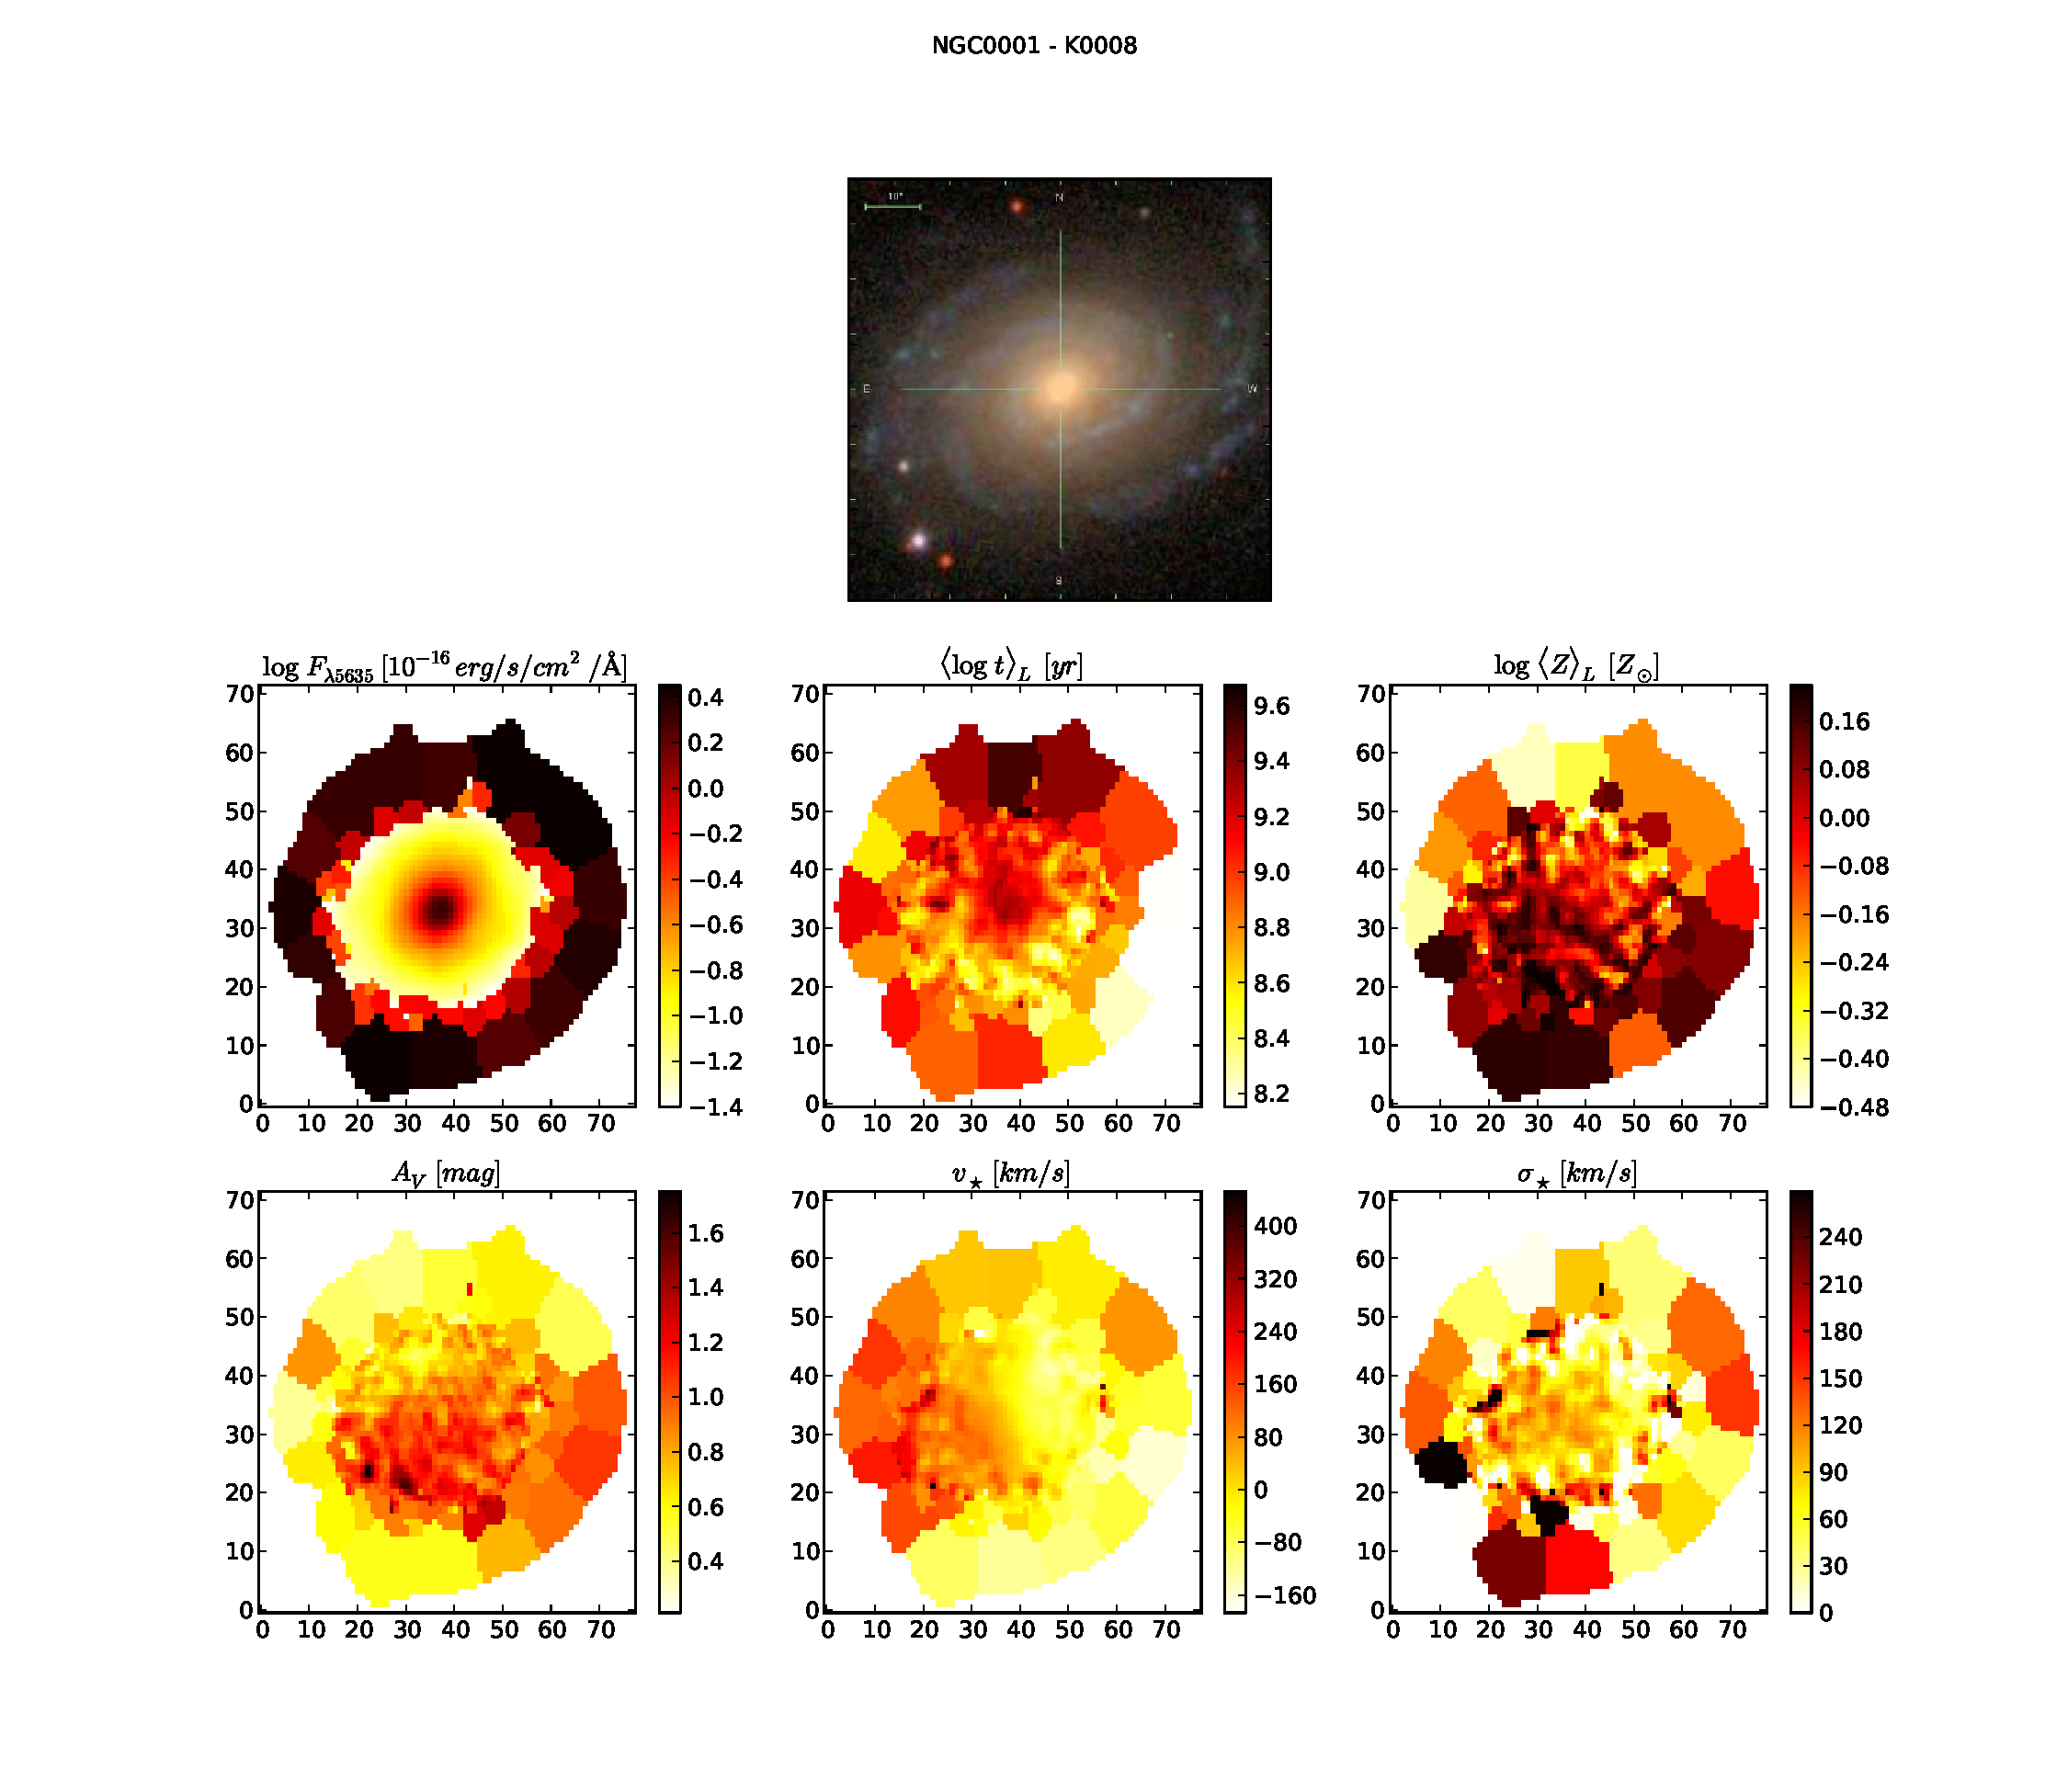
\includegraphics[width=1.\textwidth]{figuras/K0008-apresent.pdf}
    \caption[Propriedades f\'isicas da gal\'axia NGC 0001.]
    {Propriedades físicas da galáxia NGC 0001. Na primeira linha a imagem do SDSS da galáxia. Na primeira imagem da
    segunda linha temos o valor do fluxo observado em 5635 \AA, usado para a normalização dos espectros de cada zona. Da
    segunda imagem da segunda linha em diante temos as propriedades físicas que serão correlacionadas com as PCs. São
    elas: $\log\ t$, $\log\ Z$, $A_V$, $v_{\star}$, $\sigma_{\star}$.}
    \label{fig:K0008apresent}
\end{figure}

\begin{figure}
    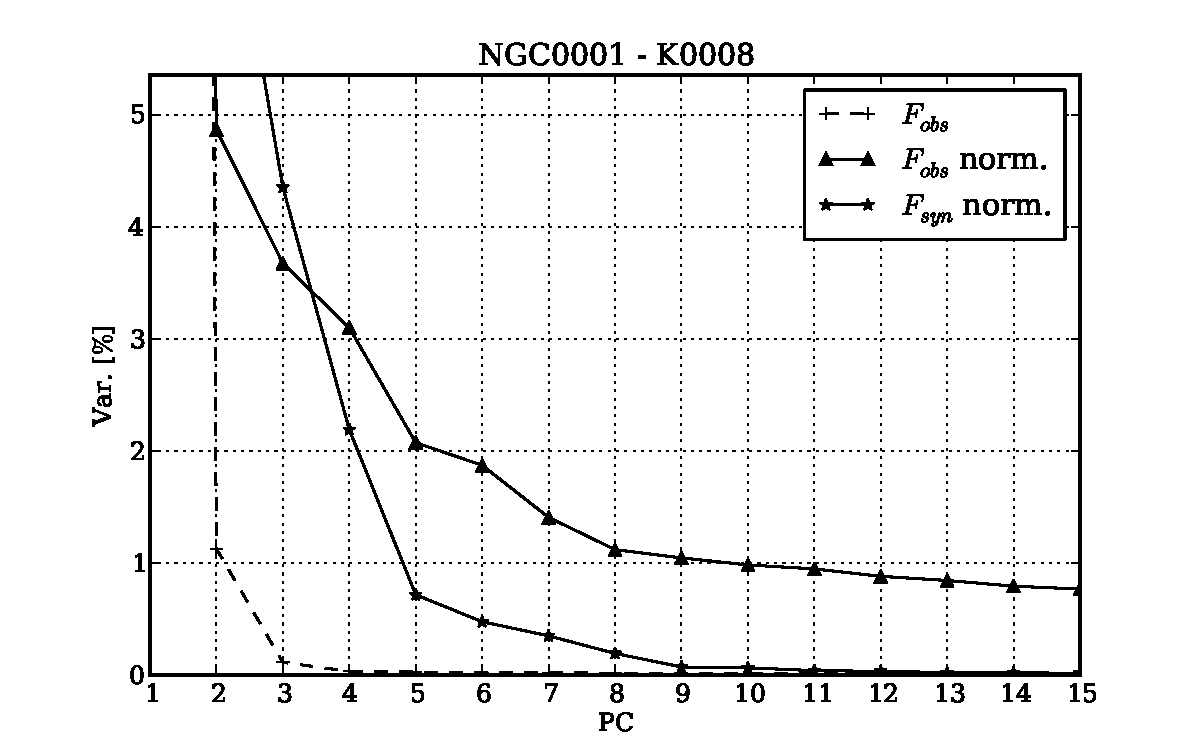
\includegraphics[height=0.33\textheight]{figuras/K0008-screetest.pdf}
    \caption[Scree test comparativo entre 3 PCAs - NGC 0001.]
    {Scree test para 3 análises PCA da galáxia NGC 0001 (CALIFA 8). Com marcações de triângulos vemos as PCs
    resultantes do PCA com os espectros observados normalizados. As variâncias das PCs marcadas com estrela representam
    o PCA com os espectros sintéticos normalizados. Para comparação plotamos as PCs do caso sem normalização usando
    linha pontilhada.}
    \label{fig:K0008scree}
\end{figure}

\begin{figure}
    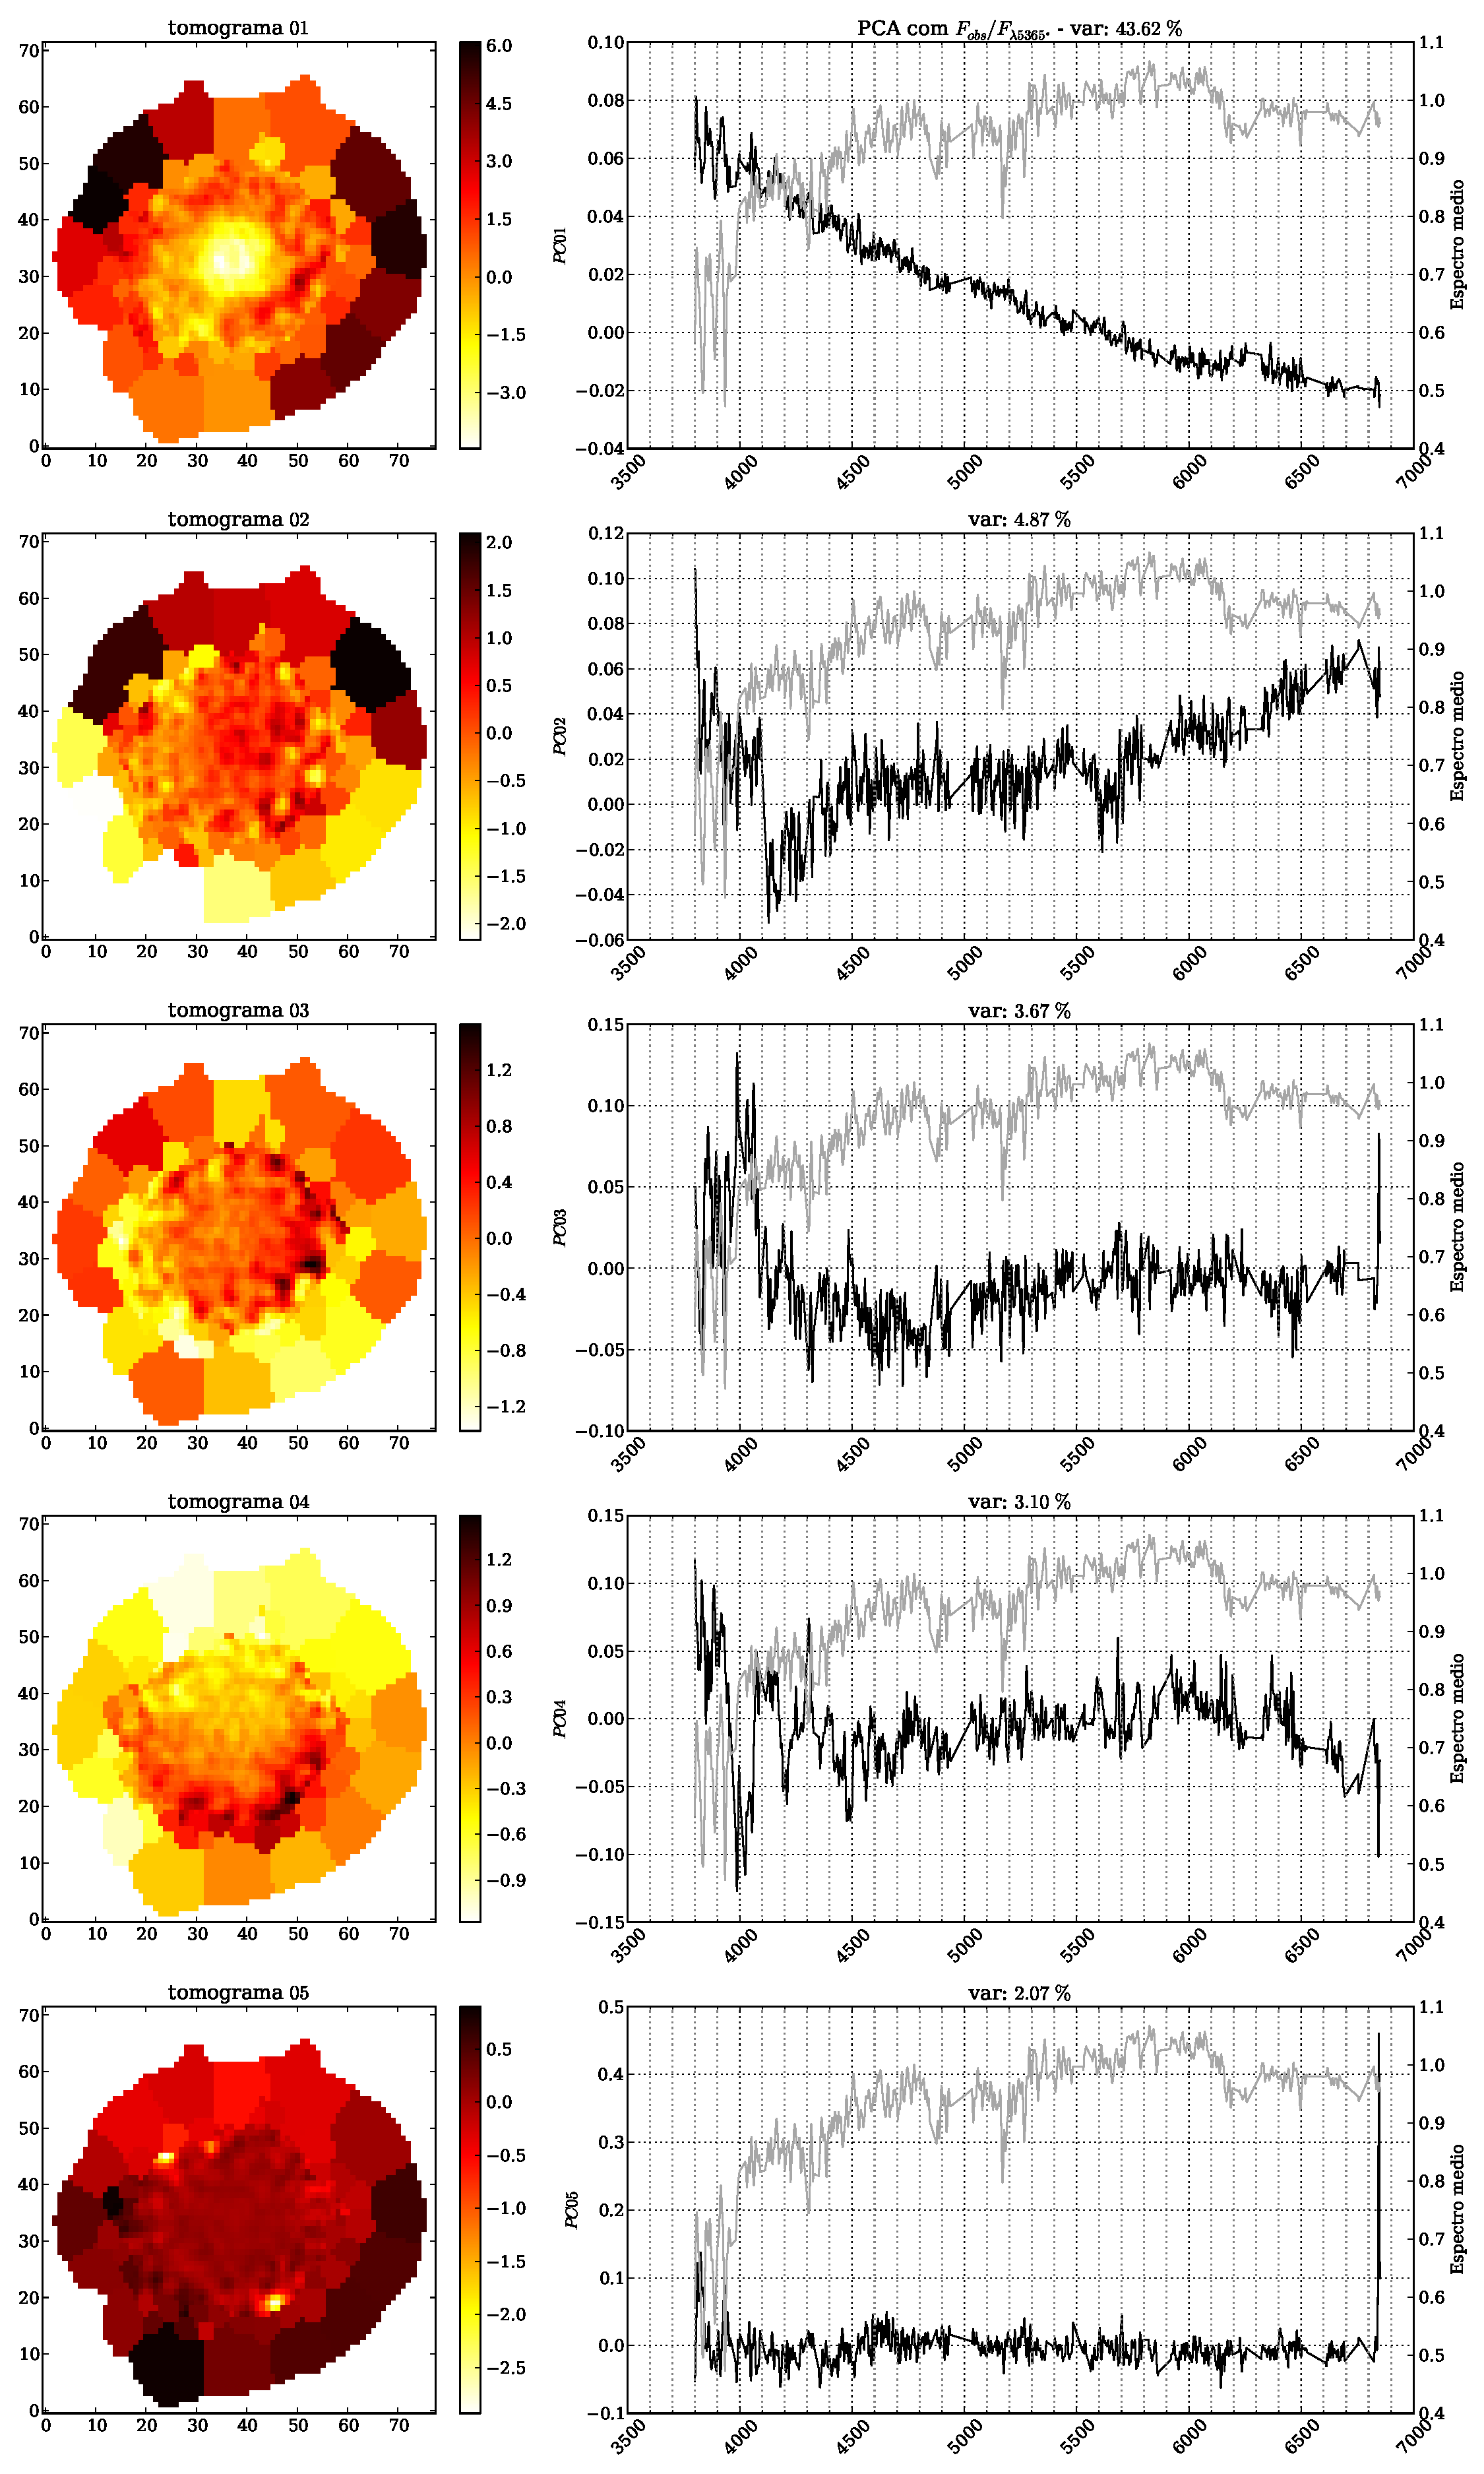
\includegraphics[width=0.85\textwidth]{figuras/K0008-tomo-obs-norm.pdf}
    \caption[Tomogramas de 1 a 5 para o cubo $F_{obs}$ norm. - NGC 0001.]
    {Cinco primeiras PCs (e seus respectivos tomogramas) resultantes da Tomografia PCA aplicado aos espectros
    observados com normalização da galáxia NGC 0001.}
    \label{fig:K0008tomofobsnorm}
\end{figure}

\begin{figure}
    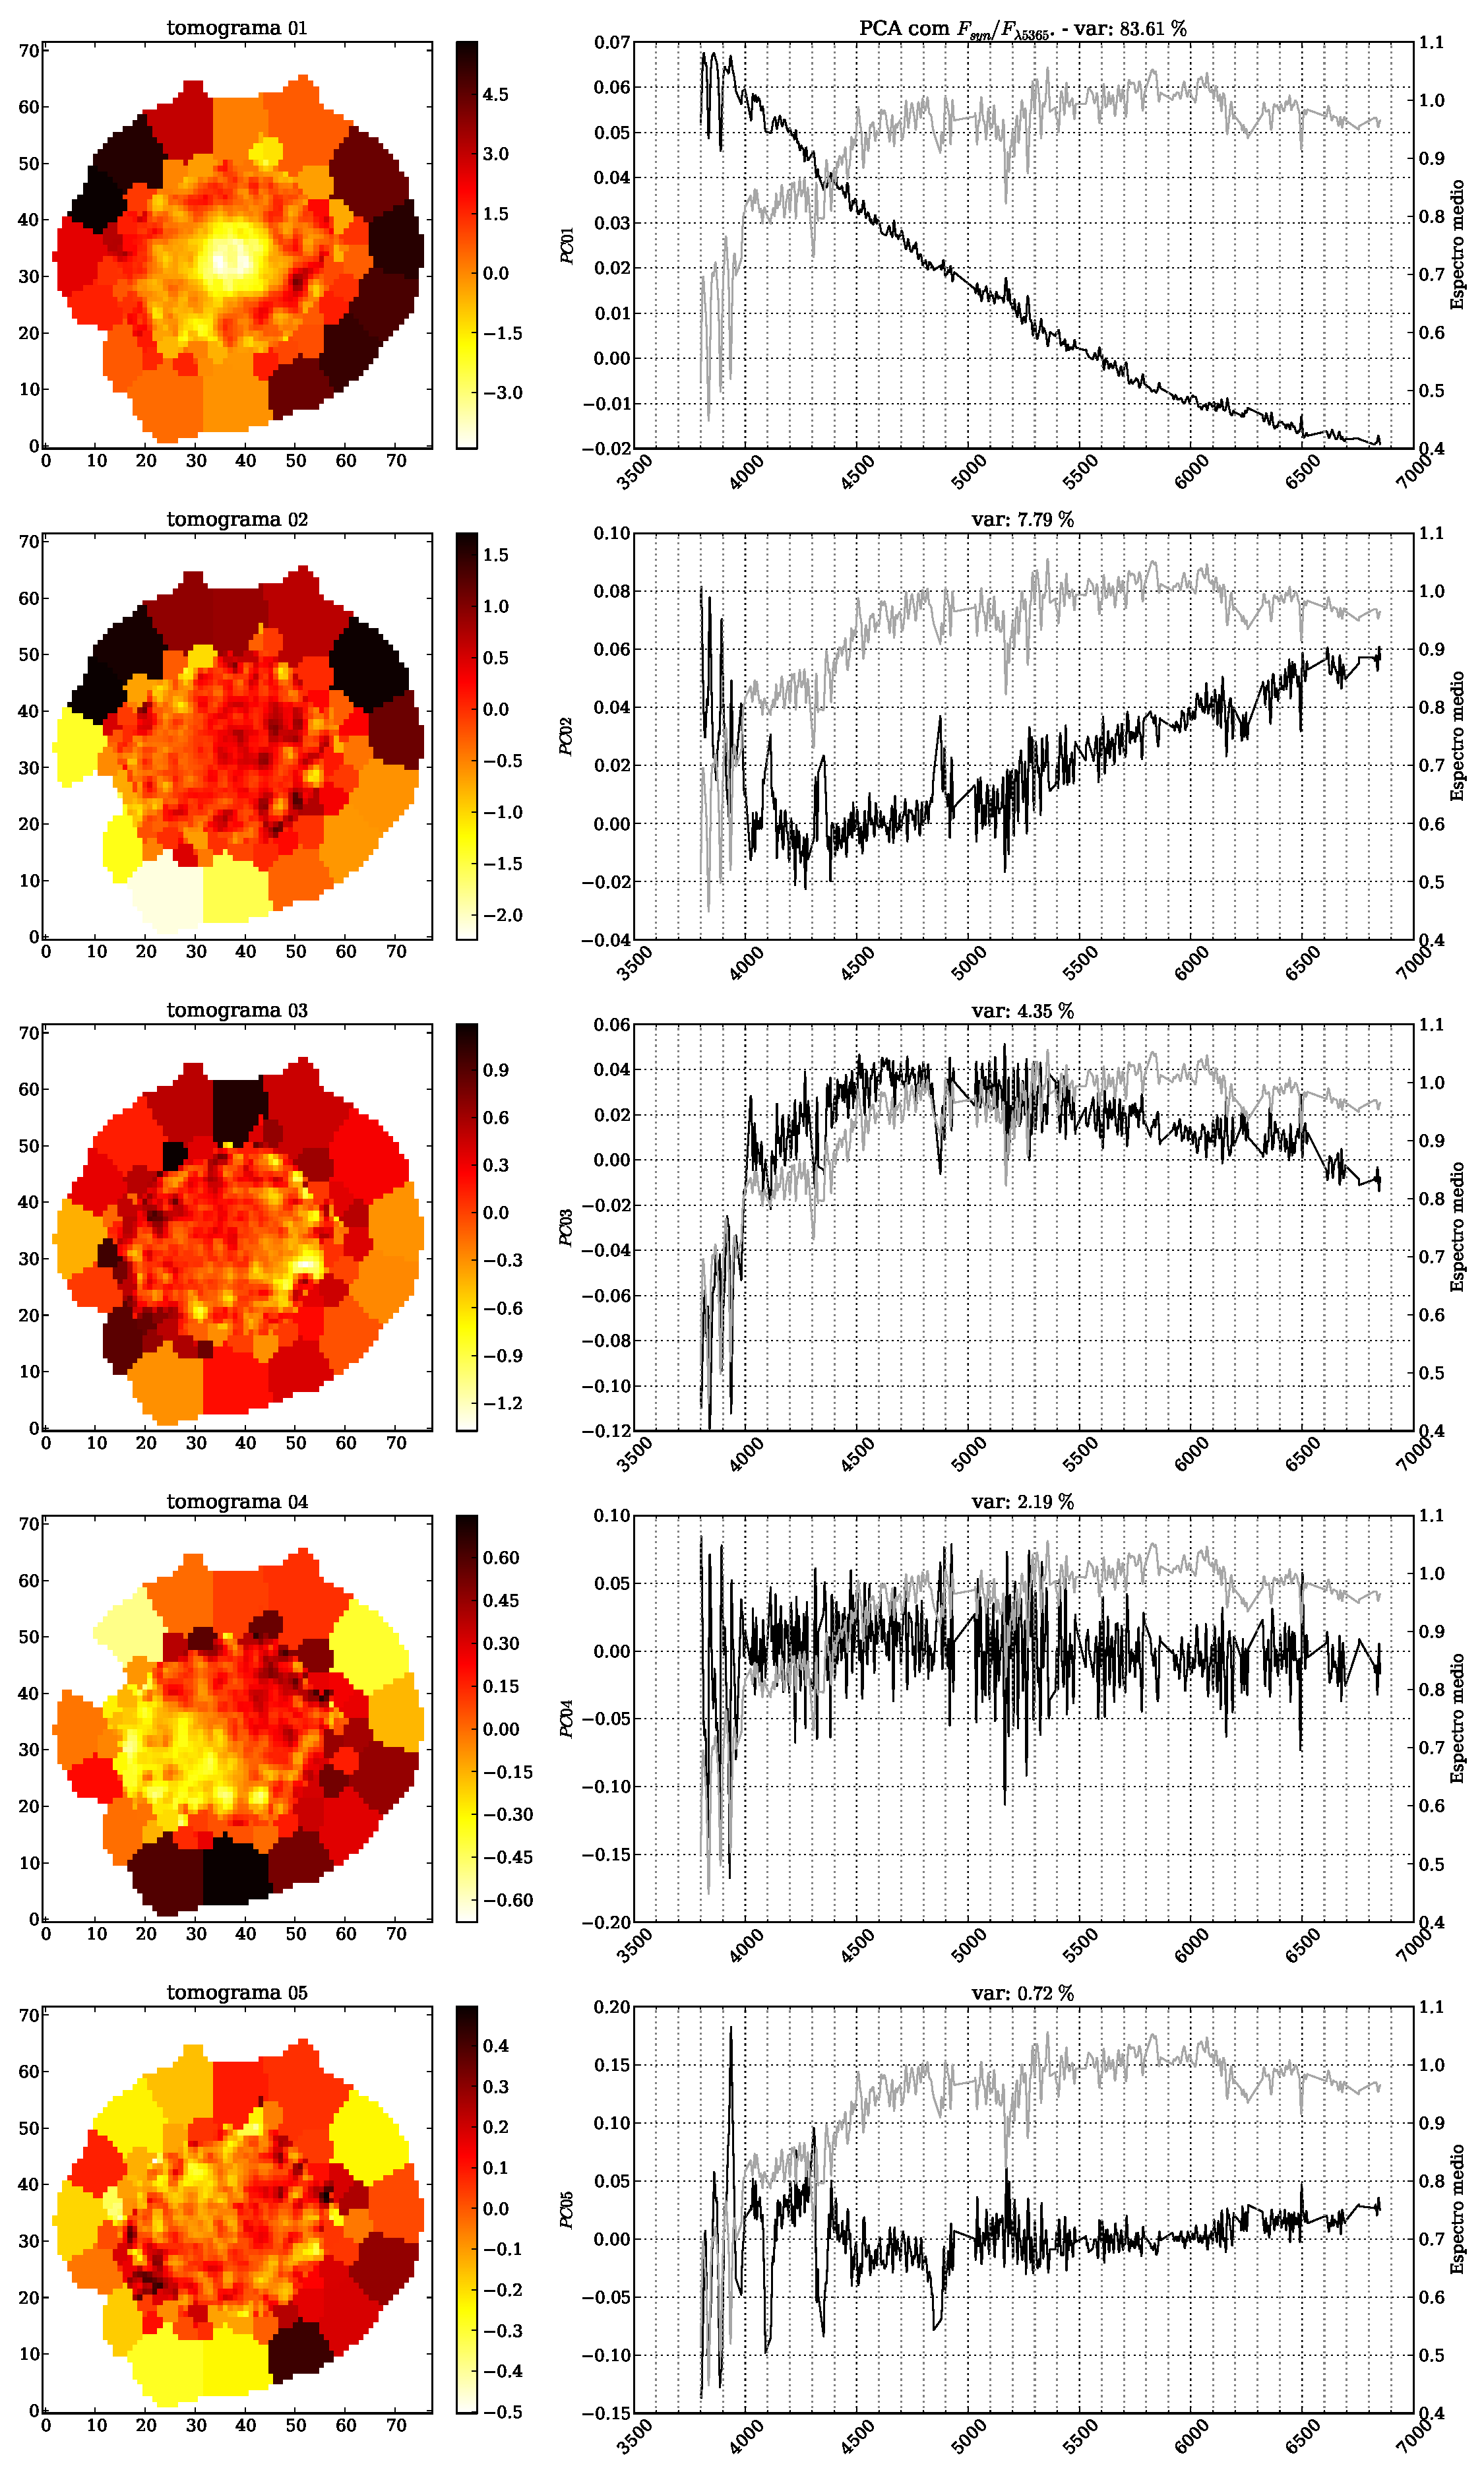
\includegraphics[width=0.85\textwidth]{figuras/K0008-tomo-syn-norm.pdf}
    \caption[Tomogramas de 1 a 5 para o cubo $F_{syn}$ norm. - NGC 0001.]
    {Cinco primeiras PCs (e seus respectivos tomogramas) resultantes da Tomografia PCA aplicado aos espectros
    sintéticos com normalização da galáxia NGC 0001.}
    \label{fig:K0008tomofsynnorm}
\end{figure}

\begin{figure}
    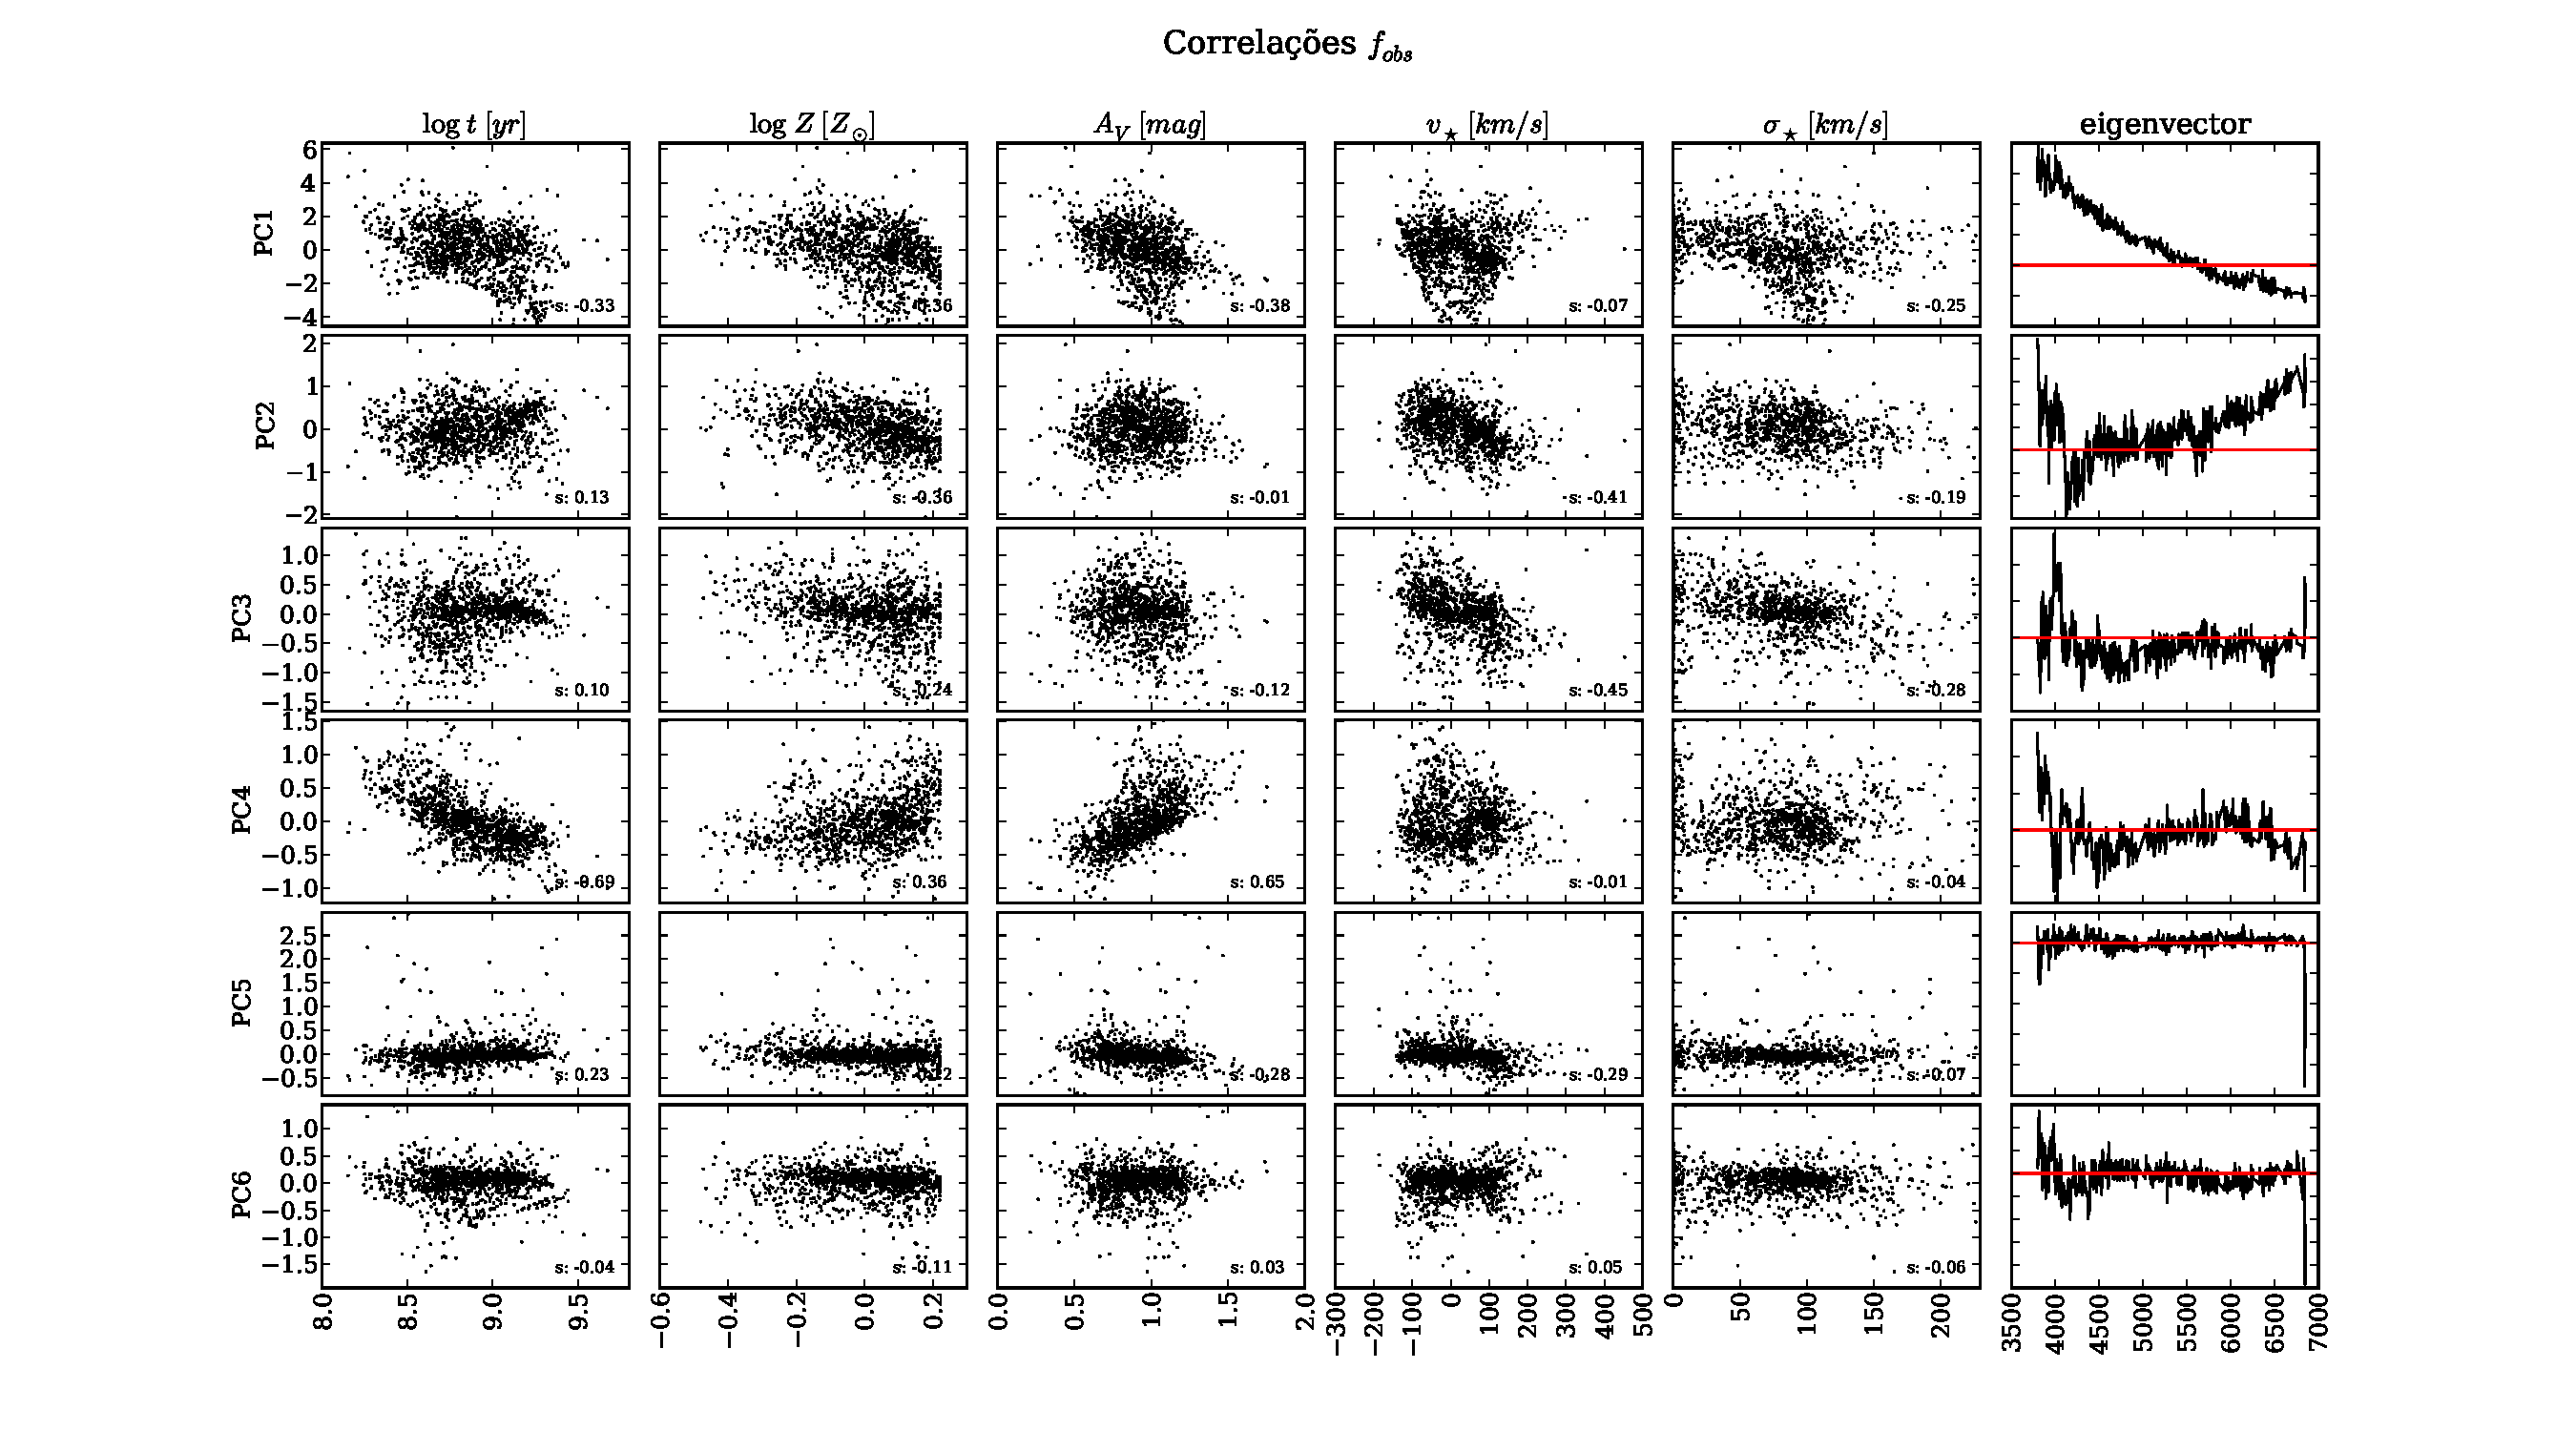
\includegraphics[width=1.3\textwidth, angle=-90]{figuras/K0008-correl-f_obs_norm-PCvsPhys.pdf}
	\caption[Correlações PCs vs. par\^ametros f\'isicos - $F_{obs}$ norm. - NGC 0001]
    {Correlações entre os pesos por zona das seis primeiras PCs do PCA feito para o cubo com os espectros observados
    normalizados e cinco parâmetros físicos.q Pela ordem de colunas da esquerda para direita temos $\log$ t, $\log\ Z$,
    $A_V$, $v_{\star}$, $\sigma_{\star}$. Na última coluna temos o autoespectro para ajudar na visualização. A linha em
    vermelho no gráfico do autoespectro serve para identificar o zero. O número dentro de cada gráfico é o coeficiente
    de correlação de Spearman.}
    \label{fig:K0008correfobsnorm}
\end{figure}

\begin{figure}
    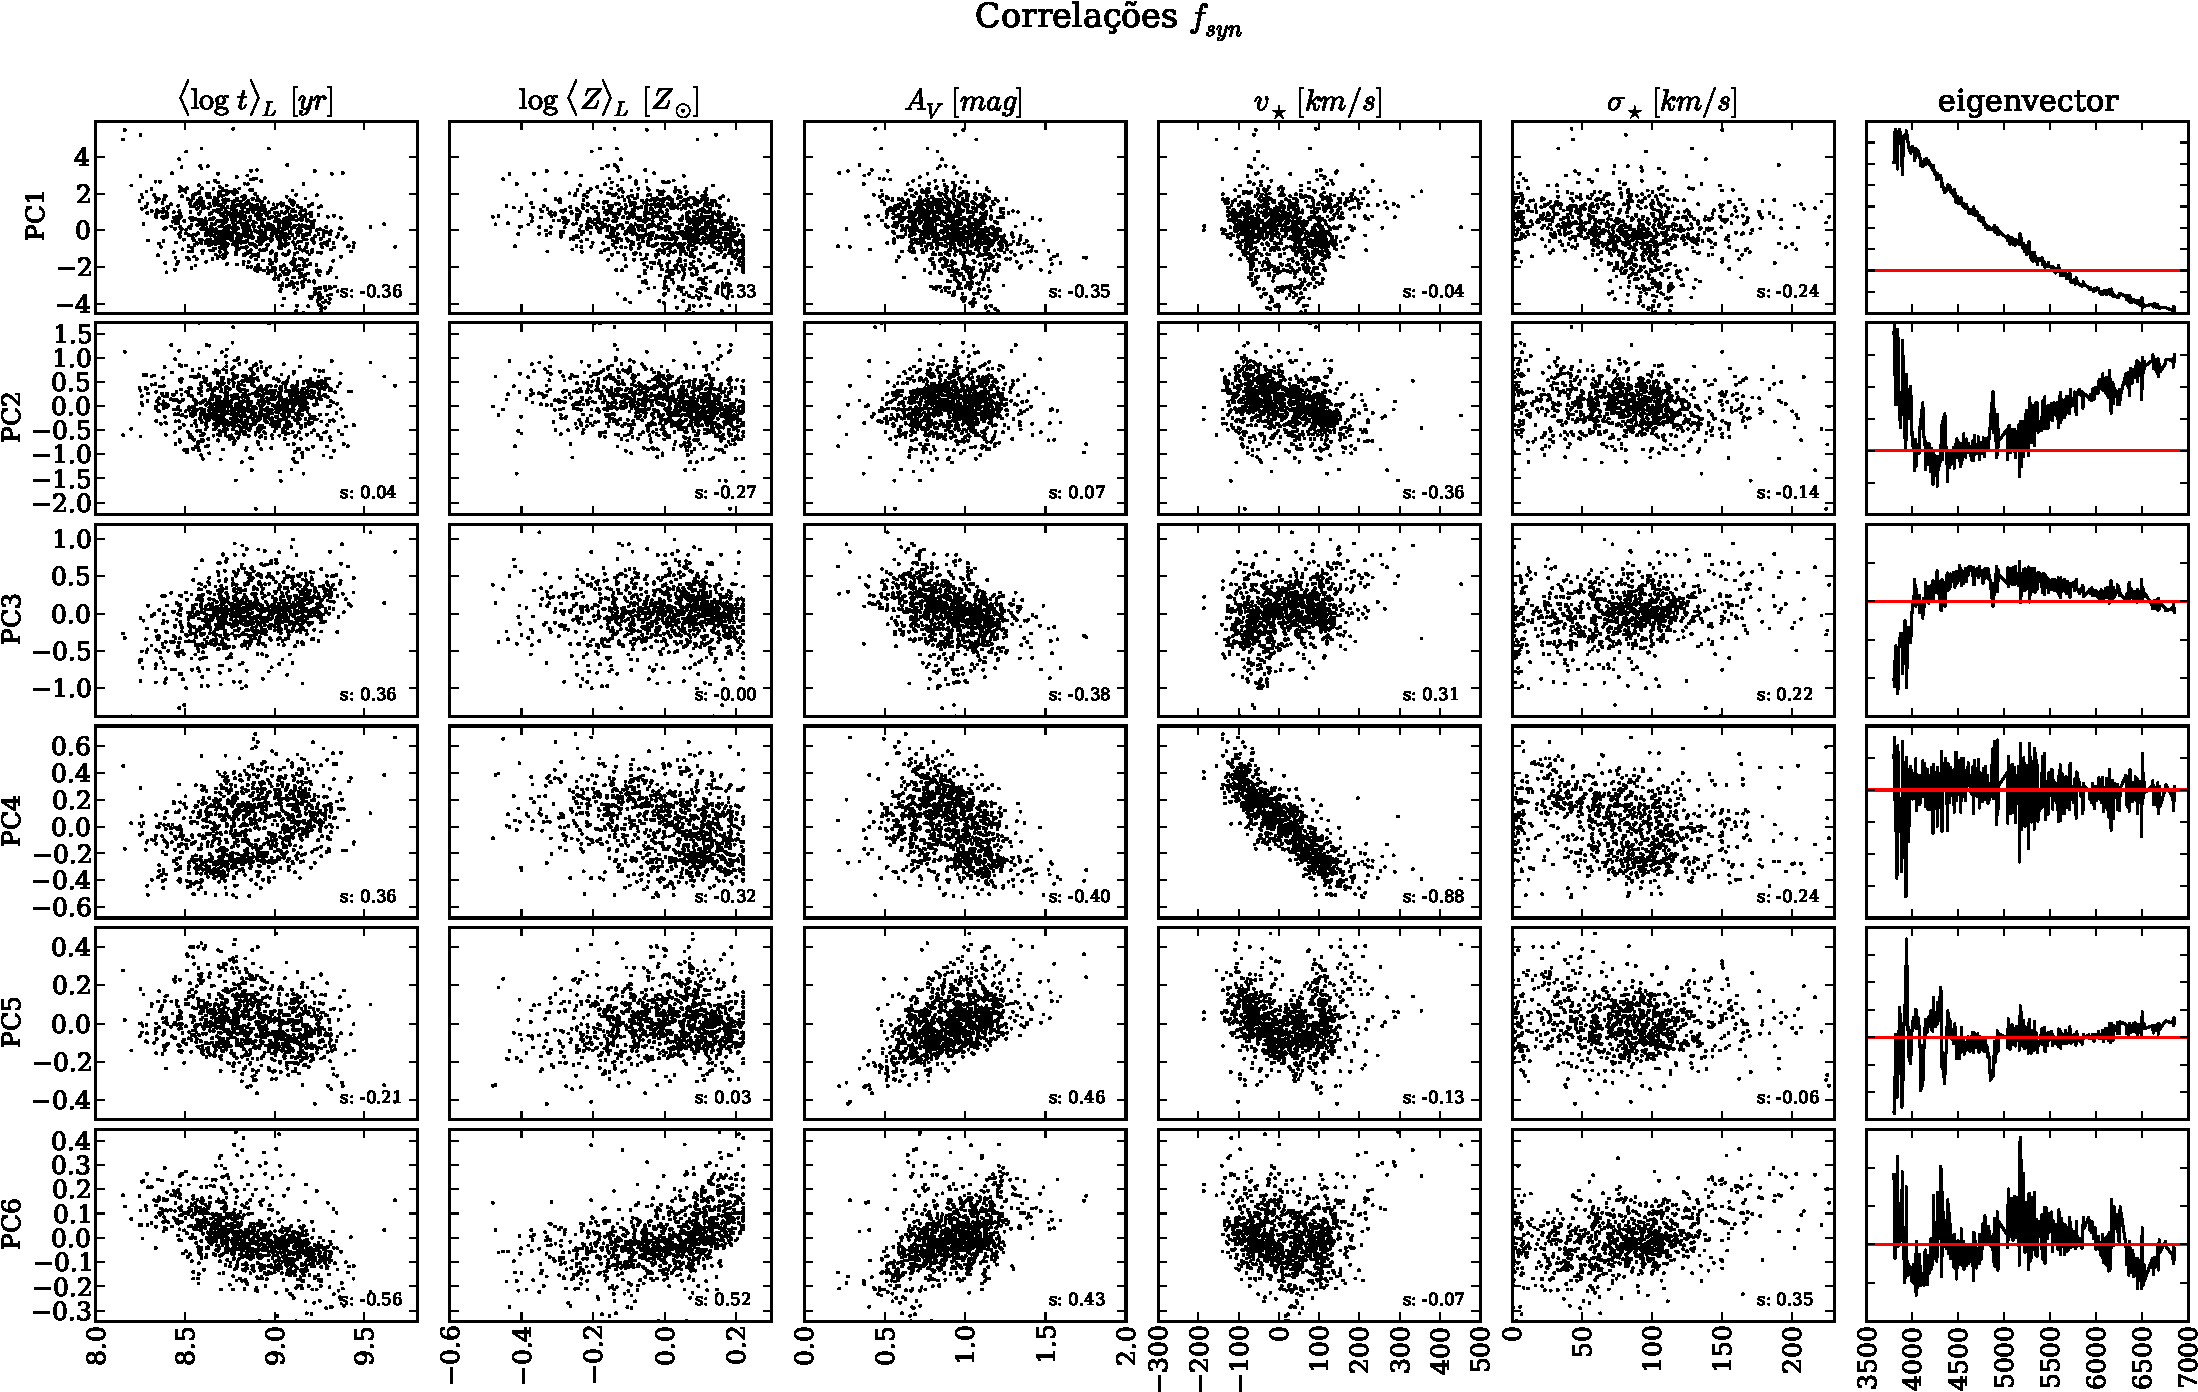
\includegraphics[width=1.3\textwidth, angle=-90]{figuras/K0008-correl-f_syn_norm-PCvsPhys.pdf}
	\caption[Correlações PCs vs. par\^ametros f\'isicos - $F_{syn}$ norm. - NGC 0001]
    {Correlações entre os pesos por zona das seis primeiras PCs do PCA feito para o cubo com os espectros sintéticos
    normalizados e cinco parâmetros físicos.q Pela ordem de colunas da esquerda para direita temos $\log$ t, $\log$ $Z /
    Z_{\odot}$, $A_V$, $v_{\star}$, $\sigma_{\star}$. Na última coluna temos o autoespectro para ajudar na visualização.
    A linha em vermelho no gráfico do autoespectro serve para identificar o zero. O número dentro de cada gráfico é o
    coeficiente de correlação de Spearman.}
    \label{fig:K0008correfsynnorm}
\end{figure}

\subsection{NGC 0776 - CALIFA 73}

\begin{figure}
    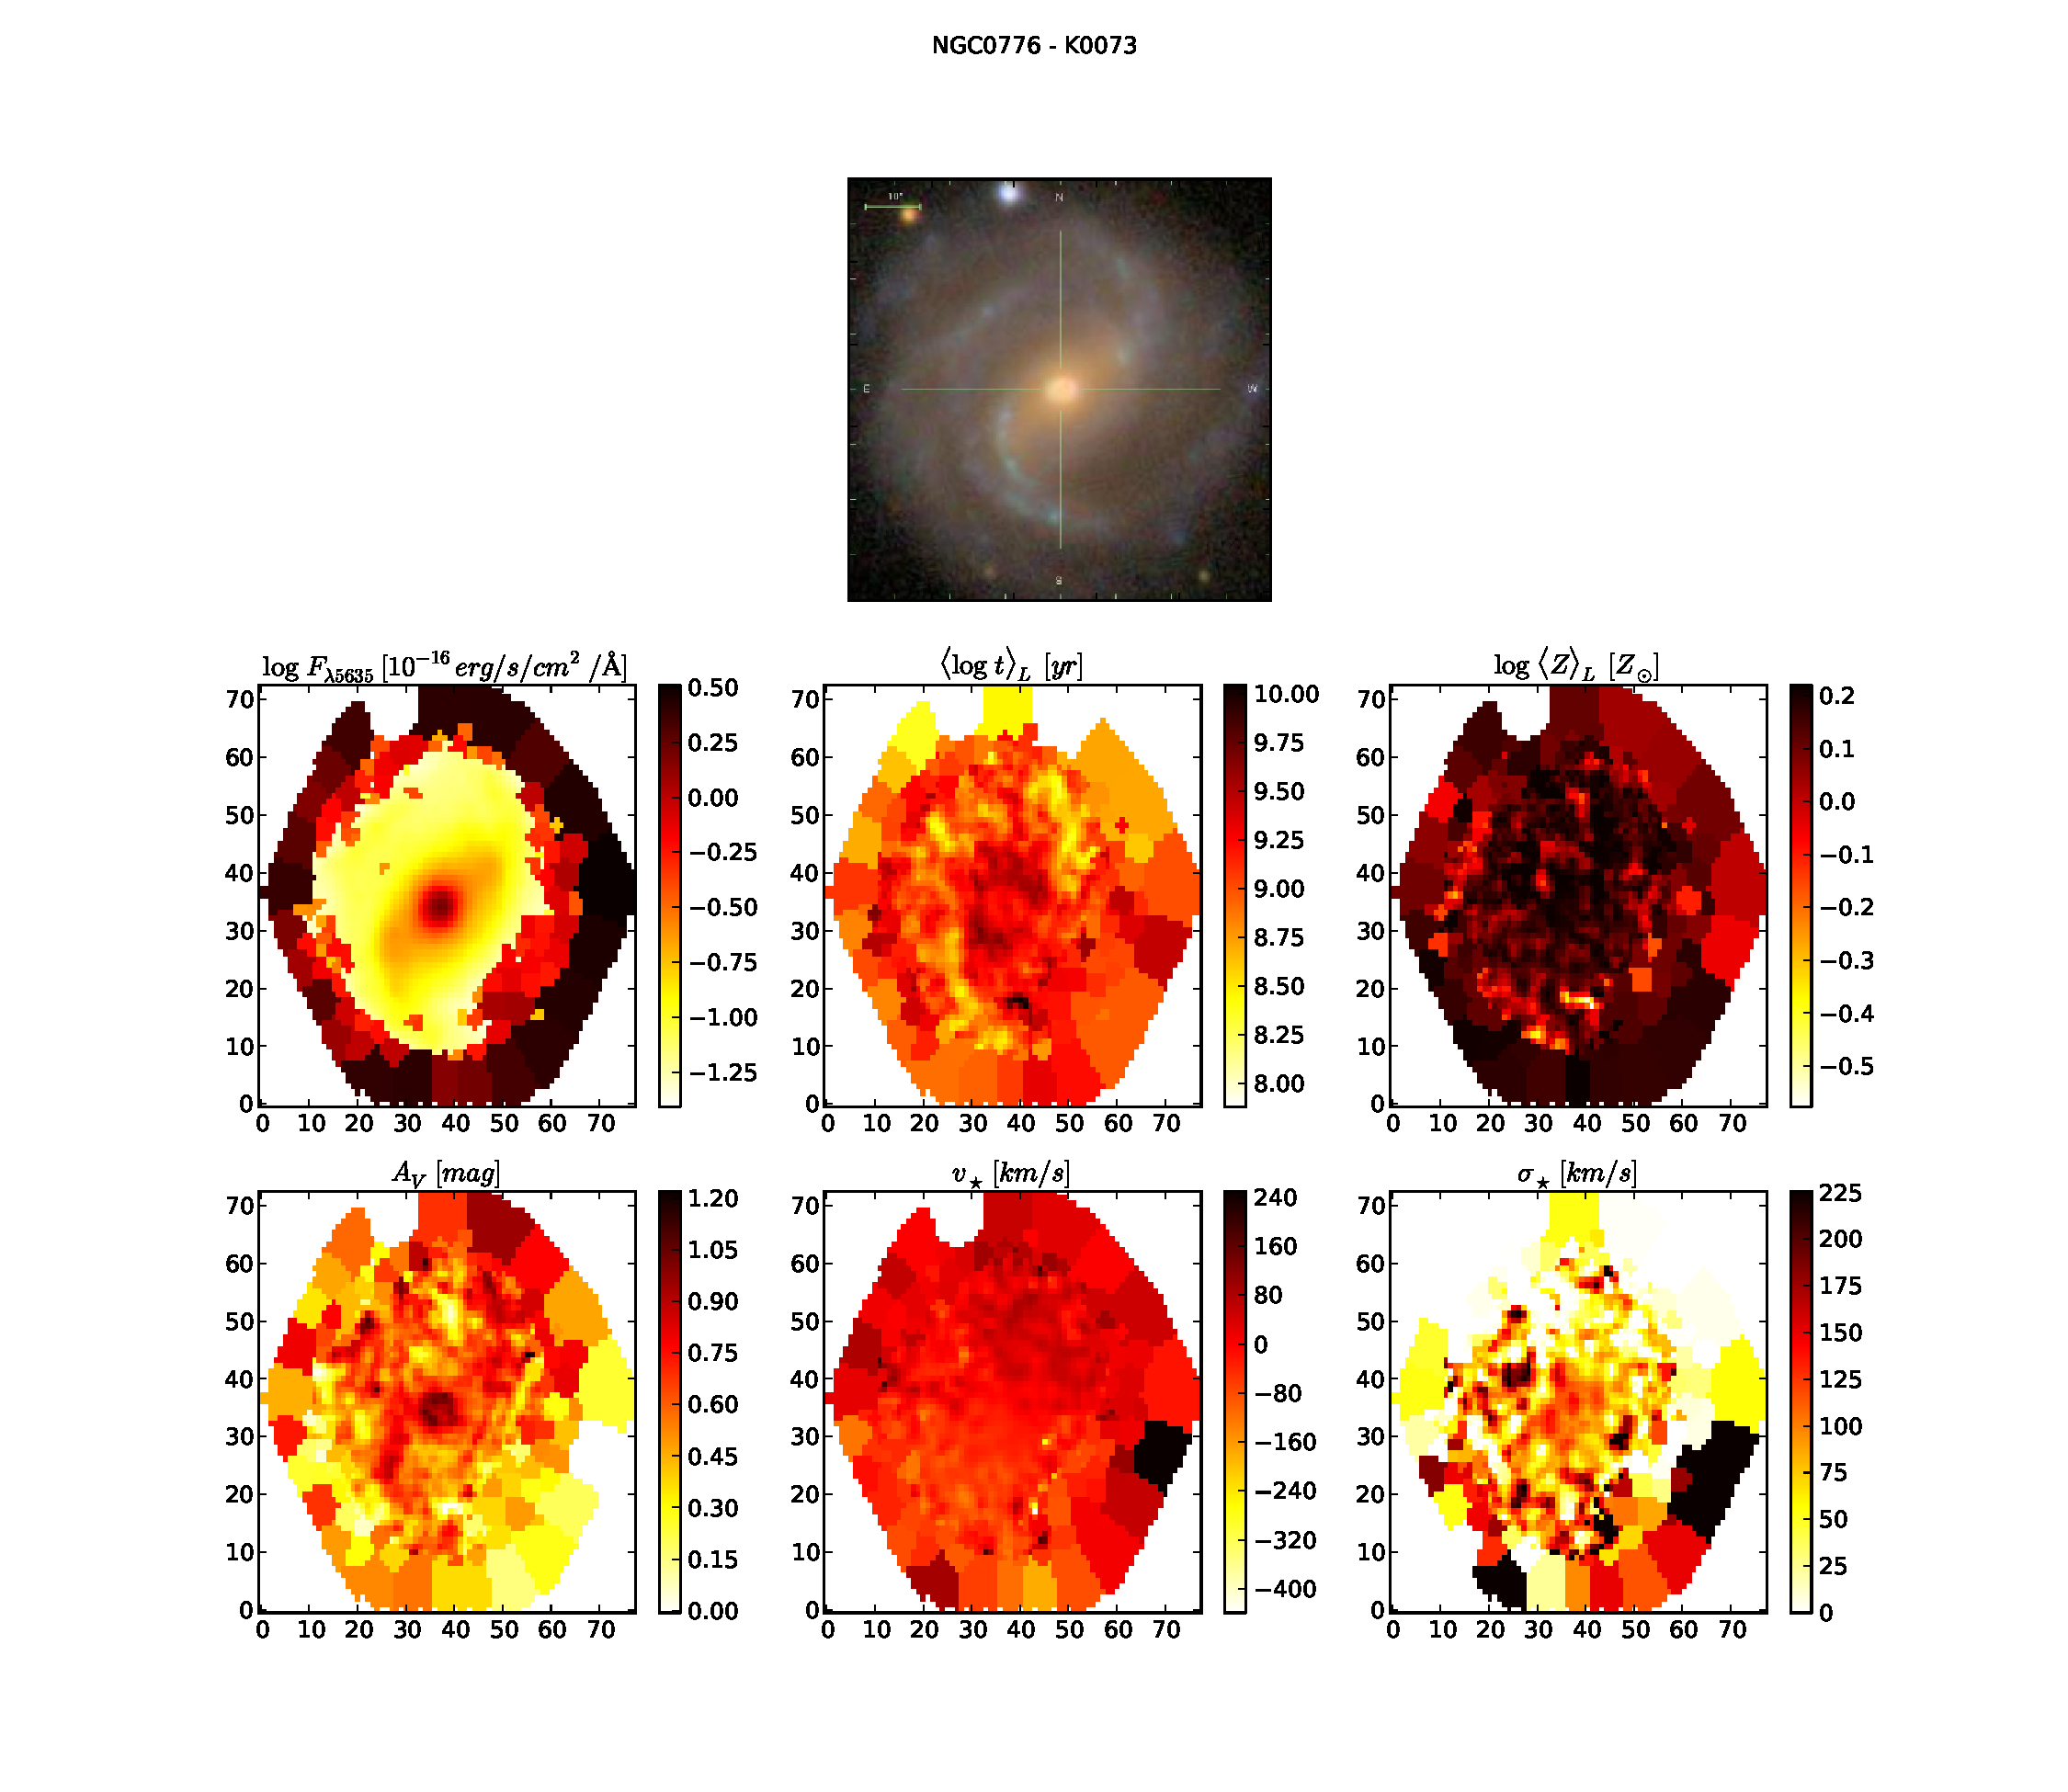
\includegraphics[width=1.\textwidth]{figuras/K0073-apresent.pdf}
    \caption[Propriedades f\'isicas da gal\'axia NGC 0776.]
    {Igual a Figura \ref{fig:K0008apresent} para a galáxia NGC 0776.}
    \label{fig:K0073apresent}
\end{figure}

\begin{figure}
    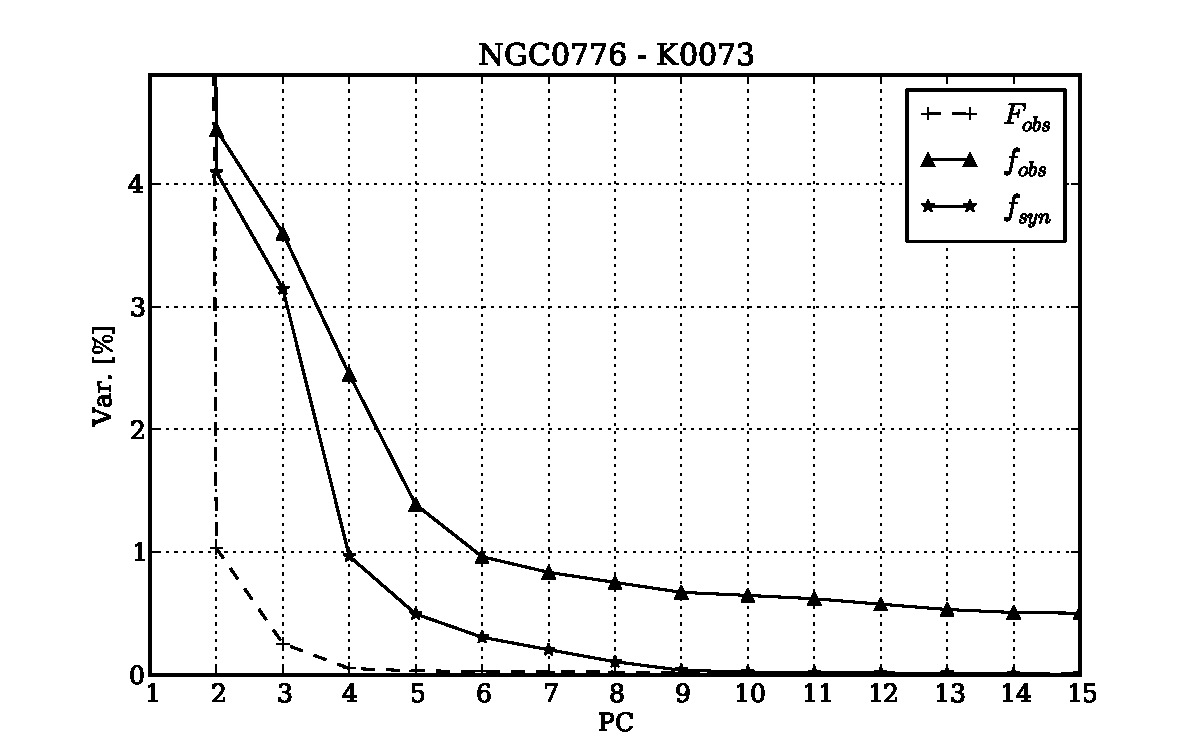
\includegraphics[height=0.33\textheight]{figuras/K0073-screetest.pdf}
    \caption[Scree test comparativo entre 3 PCAs - NGC 0776.]
    {Igual a Figura \ref{fig:K0008scree} para a galáxia NGC 0776.}
    \label{fig:K0073scree}
\end{figure}

\begin{figure}
    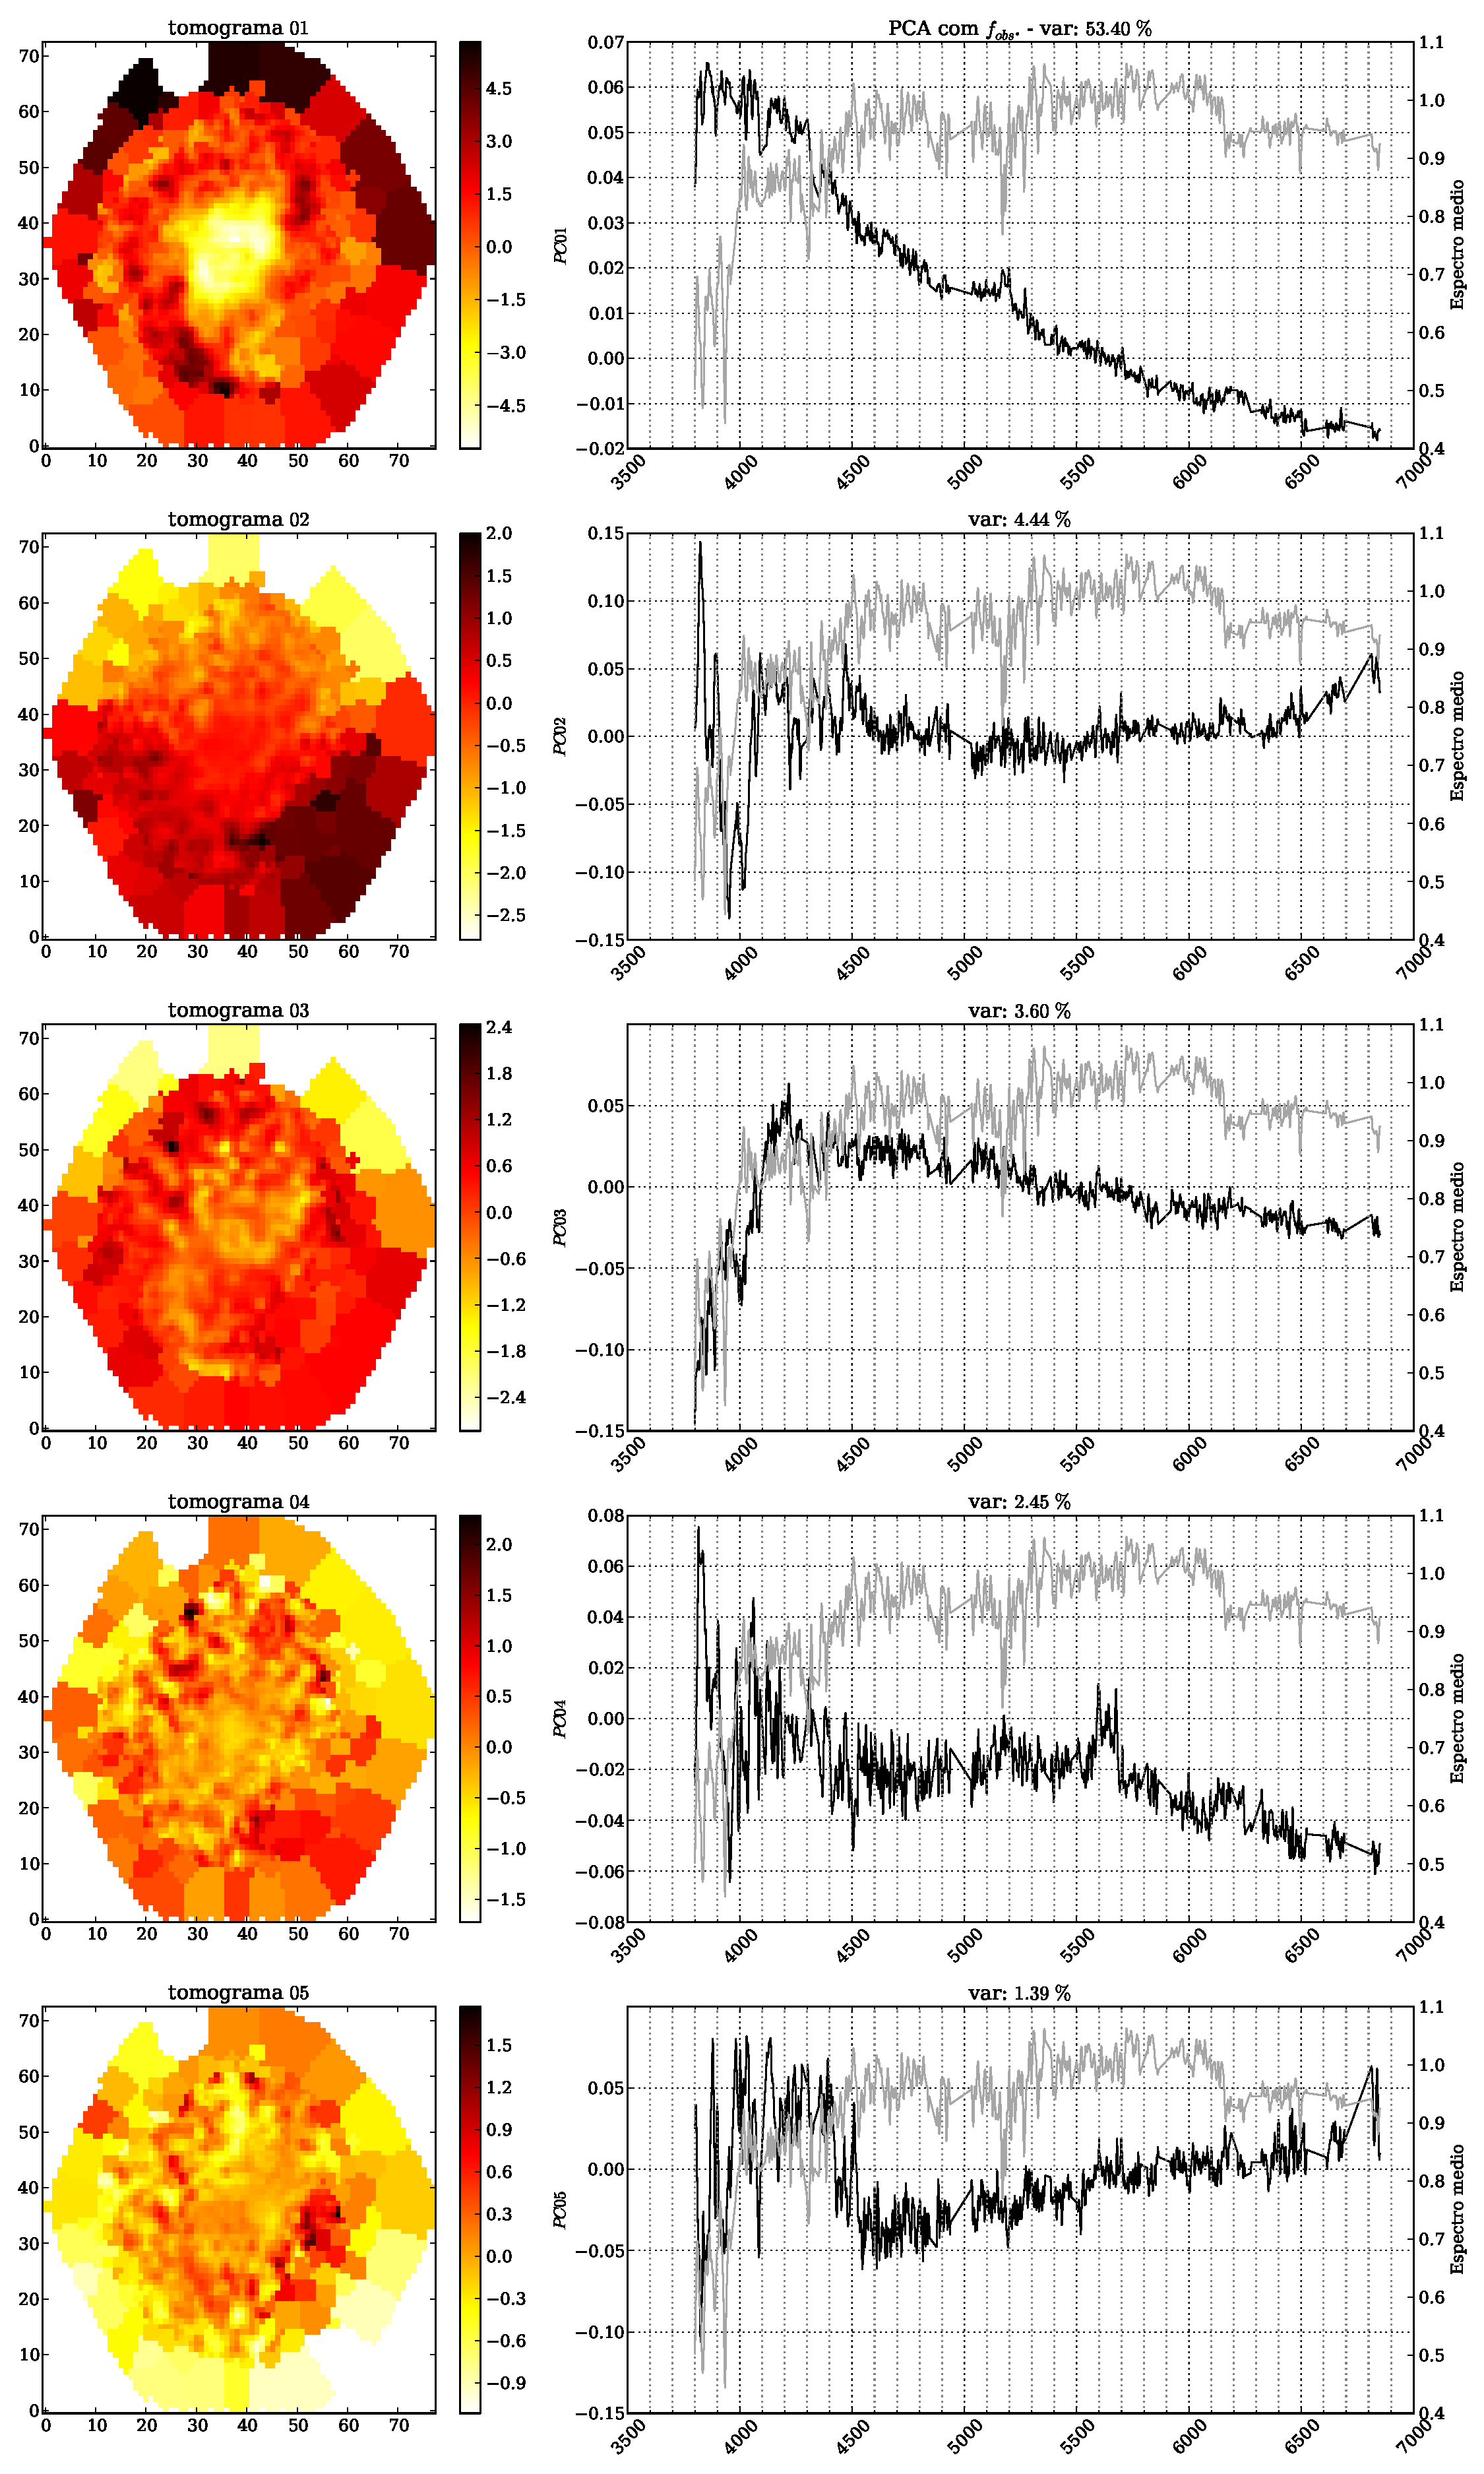
\includegraphics[width=0.85\textwidth]{figuras/K0073-tomo-obs-norm.pdf}
    \caption[Tomogramas de 1 a 5 para o cubo $F_{obs}$ norm. - NGC 0776.]
    {Igual a Figura \ref{fig:K0008tomofobsnorm} para a galáxia NGC 0776.}
    \label{fig:K0073tomofobsnorm}
\end{figure}

\begin{figure}
    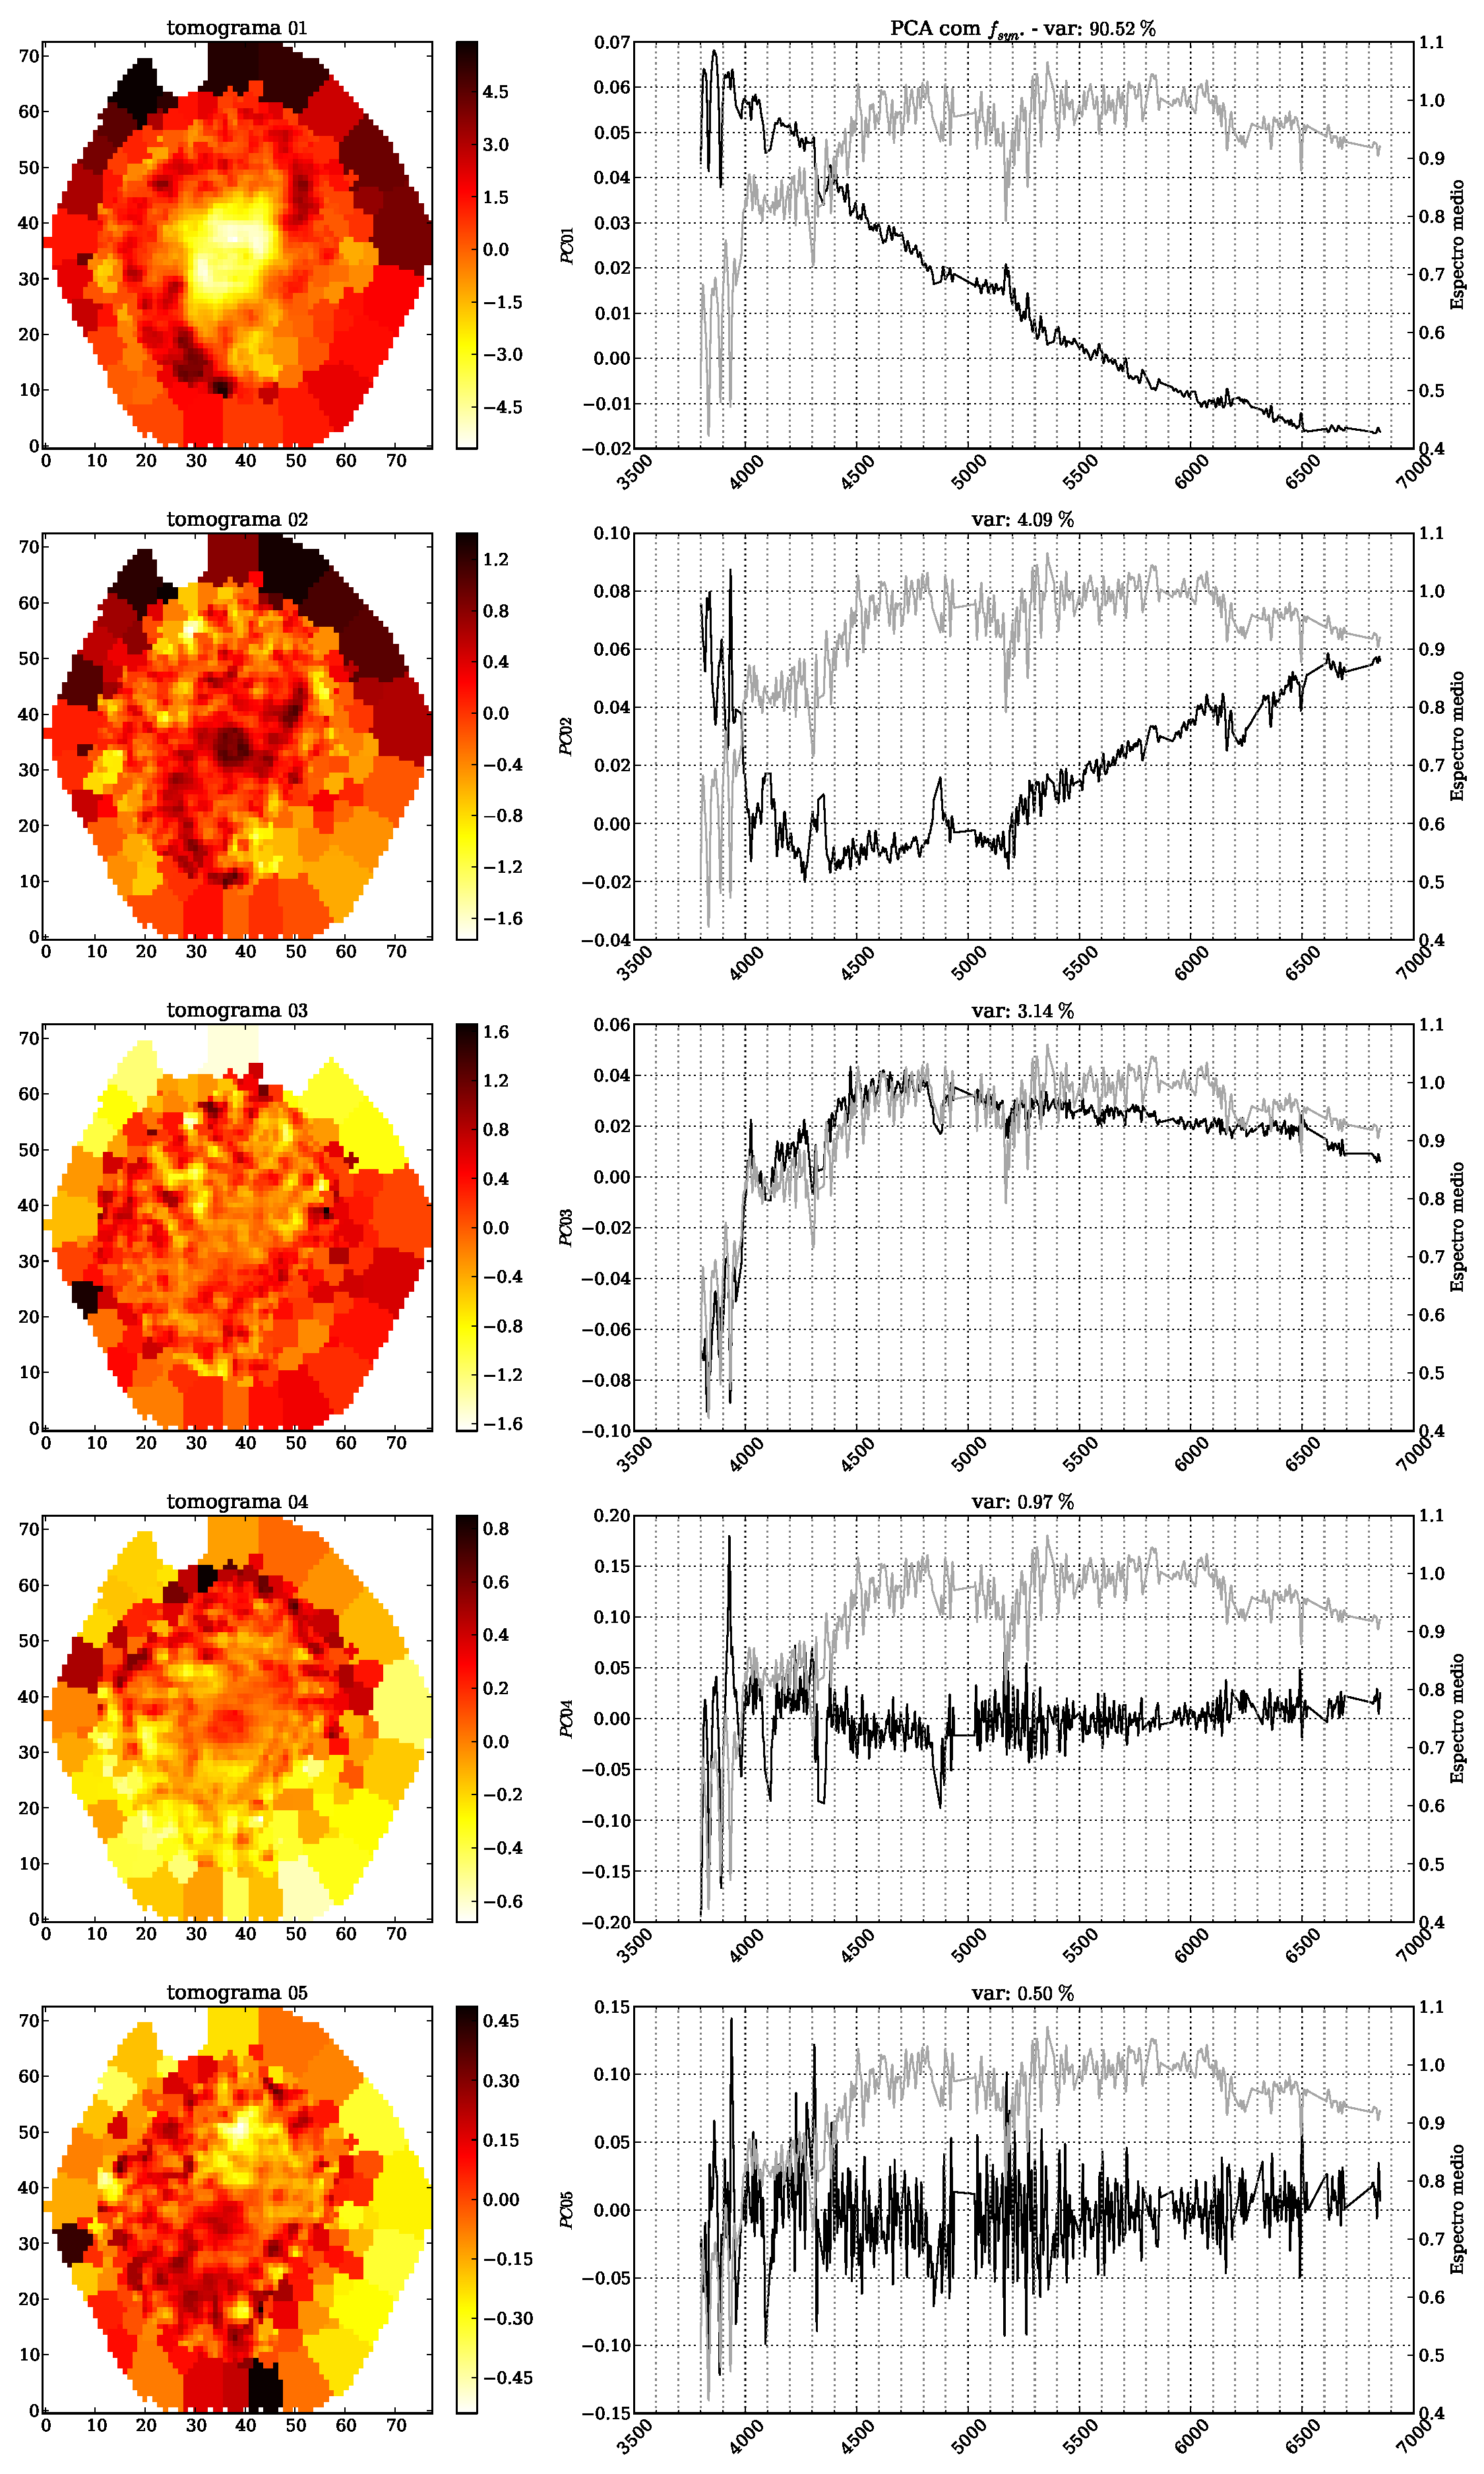
\includegraphics[width=0.85\textwidth]{figuras/K0073-tomo-syn-norm.pdf}
    \caption[Tomogramas de 1 a 5 para o cubo $F_{syn}$ norm. - NGC 0776.]
    {Igual a Figura \ref{fig:K0008tomofsynnorm} para a galáxia NGC 0776.}
    \label{fig:K0073tomofsynnorm}
\end{figure}

\begin{figure}
    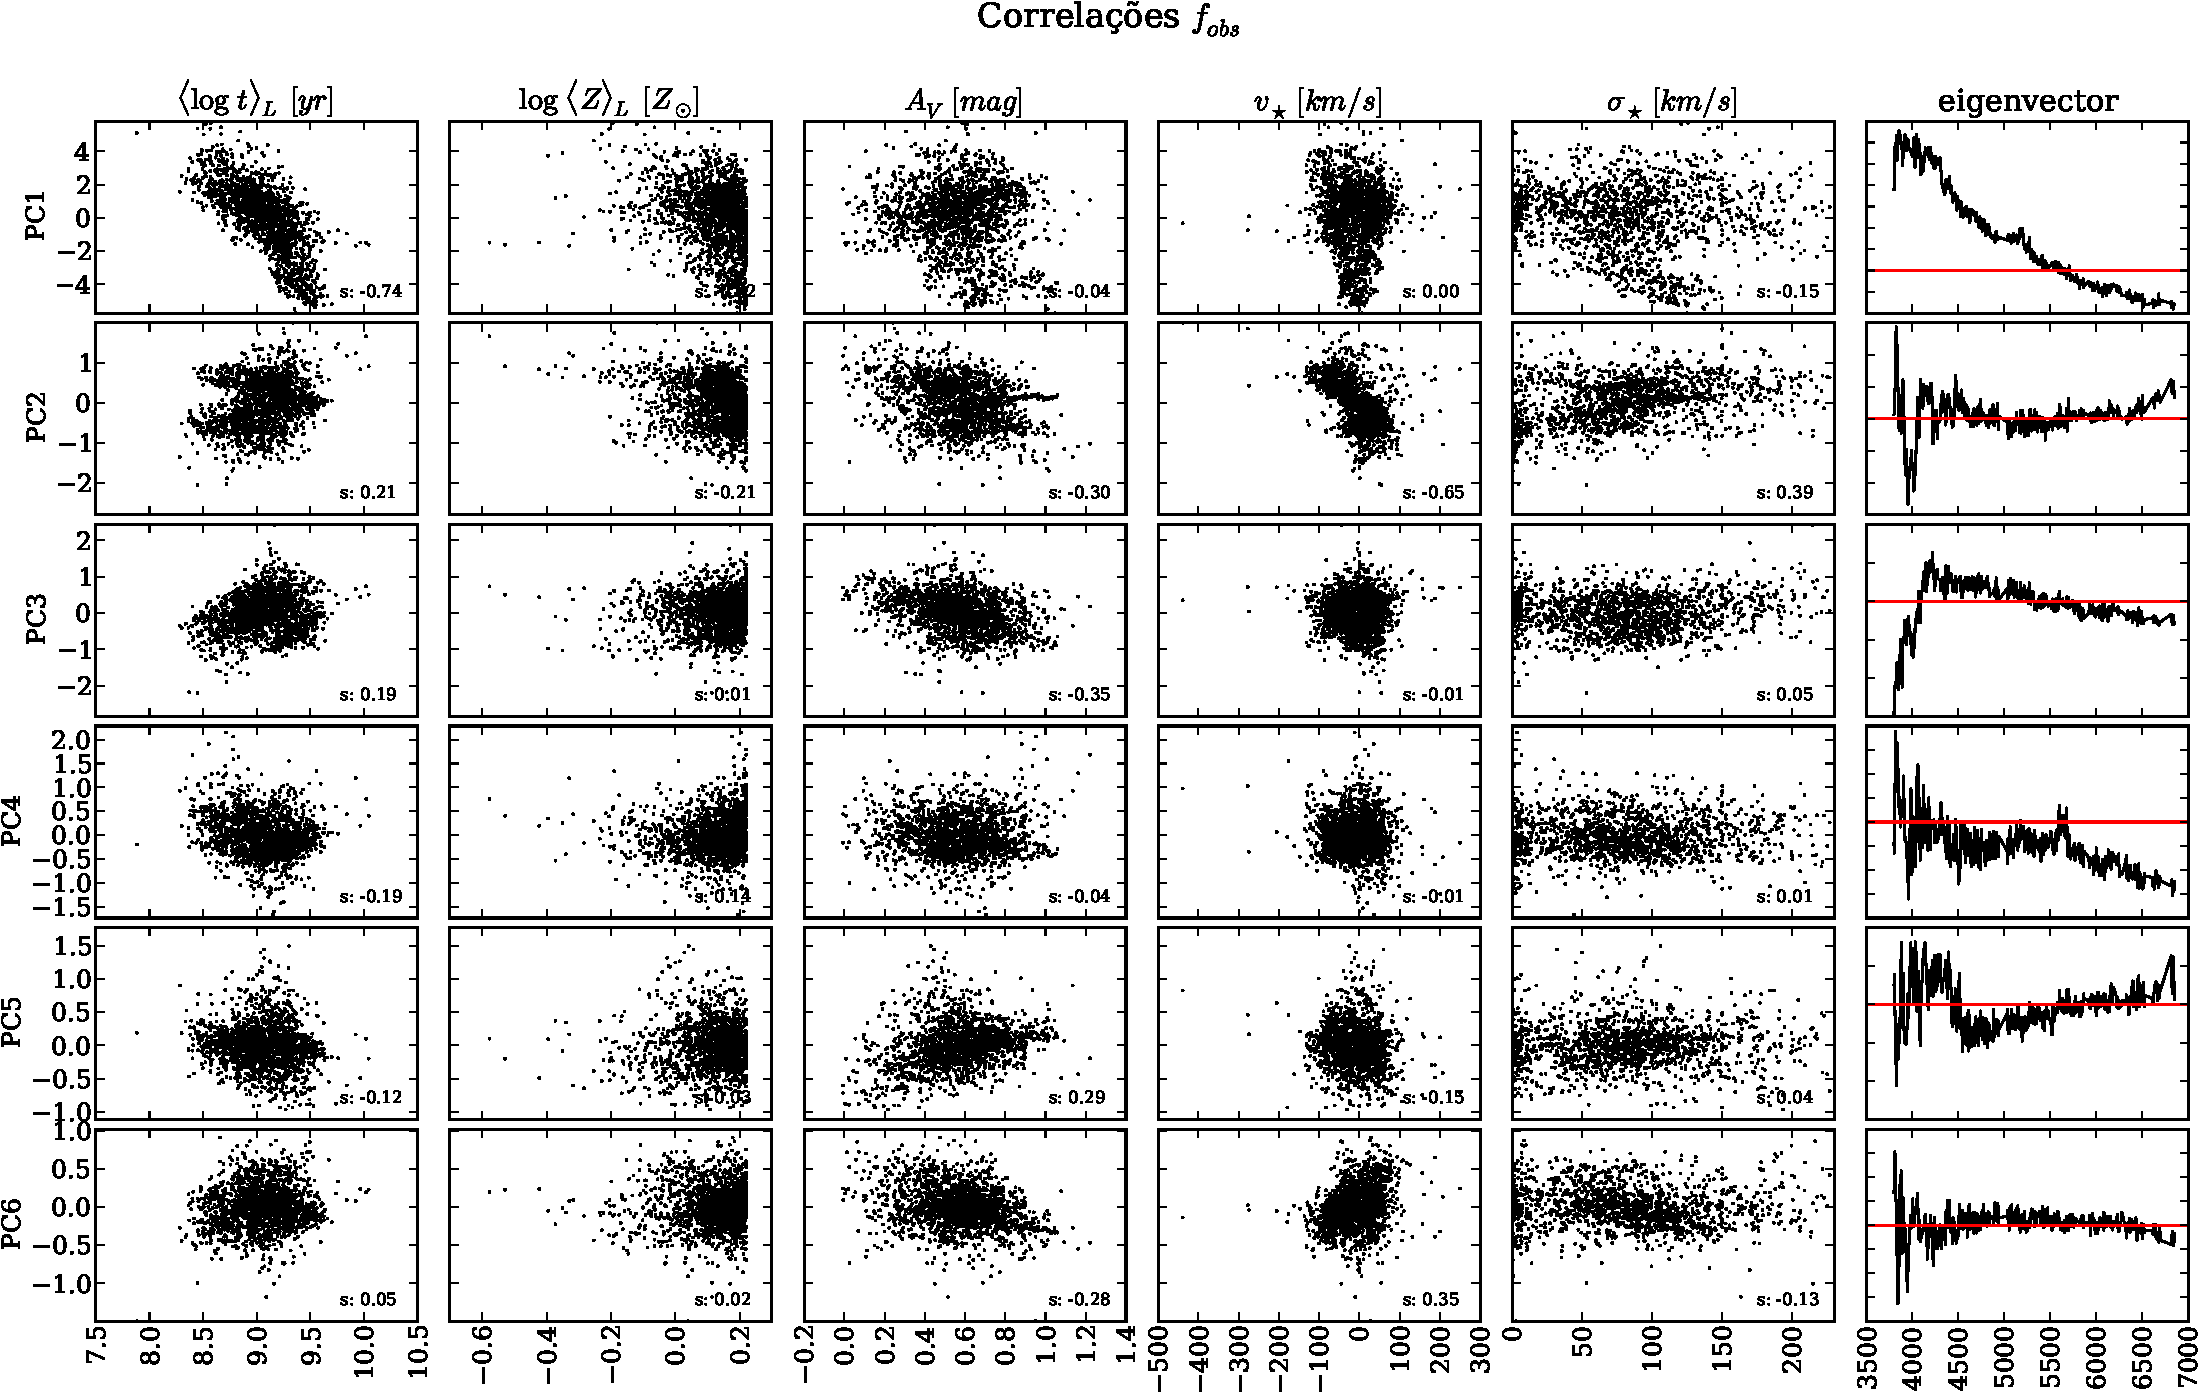
\includegraphics[width=1.3\textwidth, angle=-90]{figuras/K0073-correl-f_obs_norm-PCvsPhys.pdf}
	\caption[Correlações PCs vs. par\^ametros f\'isicos - $F_{obs}$ norm. - NGC 0001]
	{Igual a Figura \ref{fig:K0008correfobsnorm} para a galáxia NGC 0776.}
    \label{fig:K0073correfobsnorm}
\end{figure}

\begin{figure}
    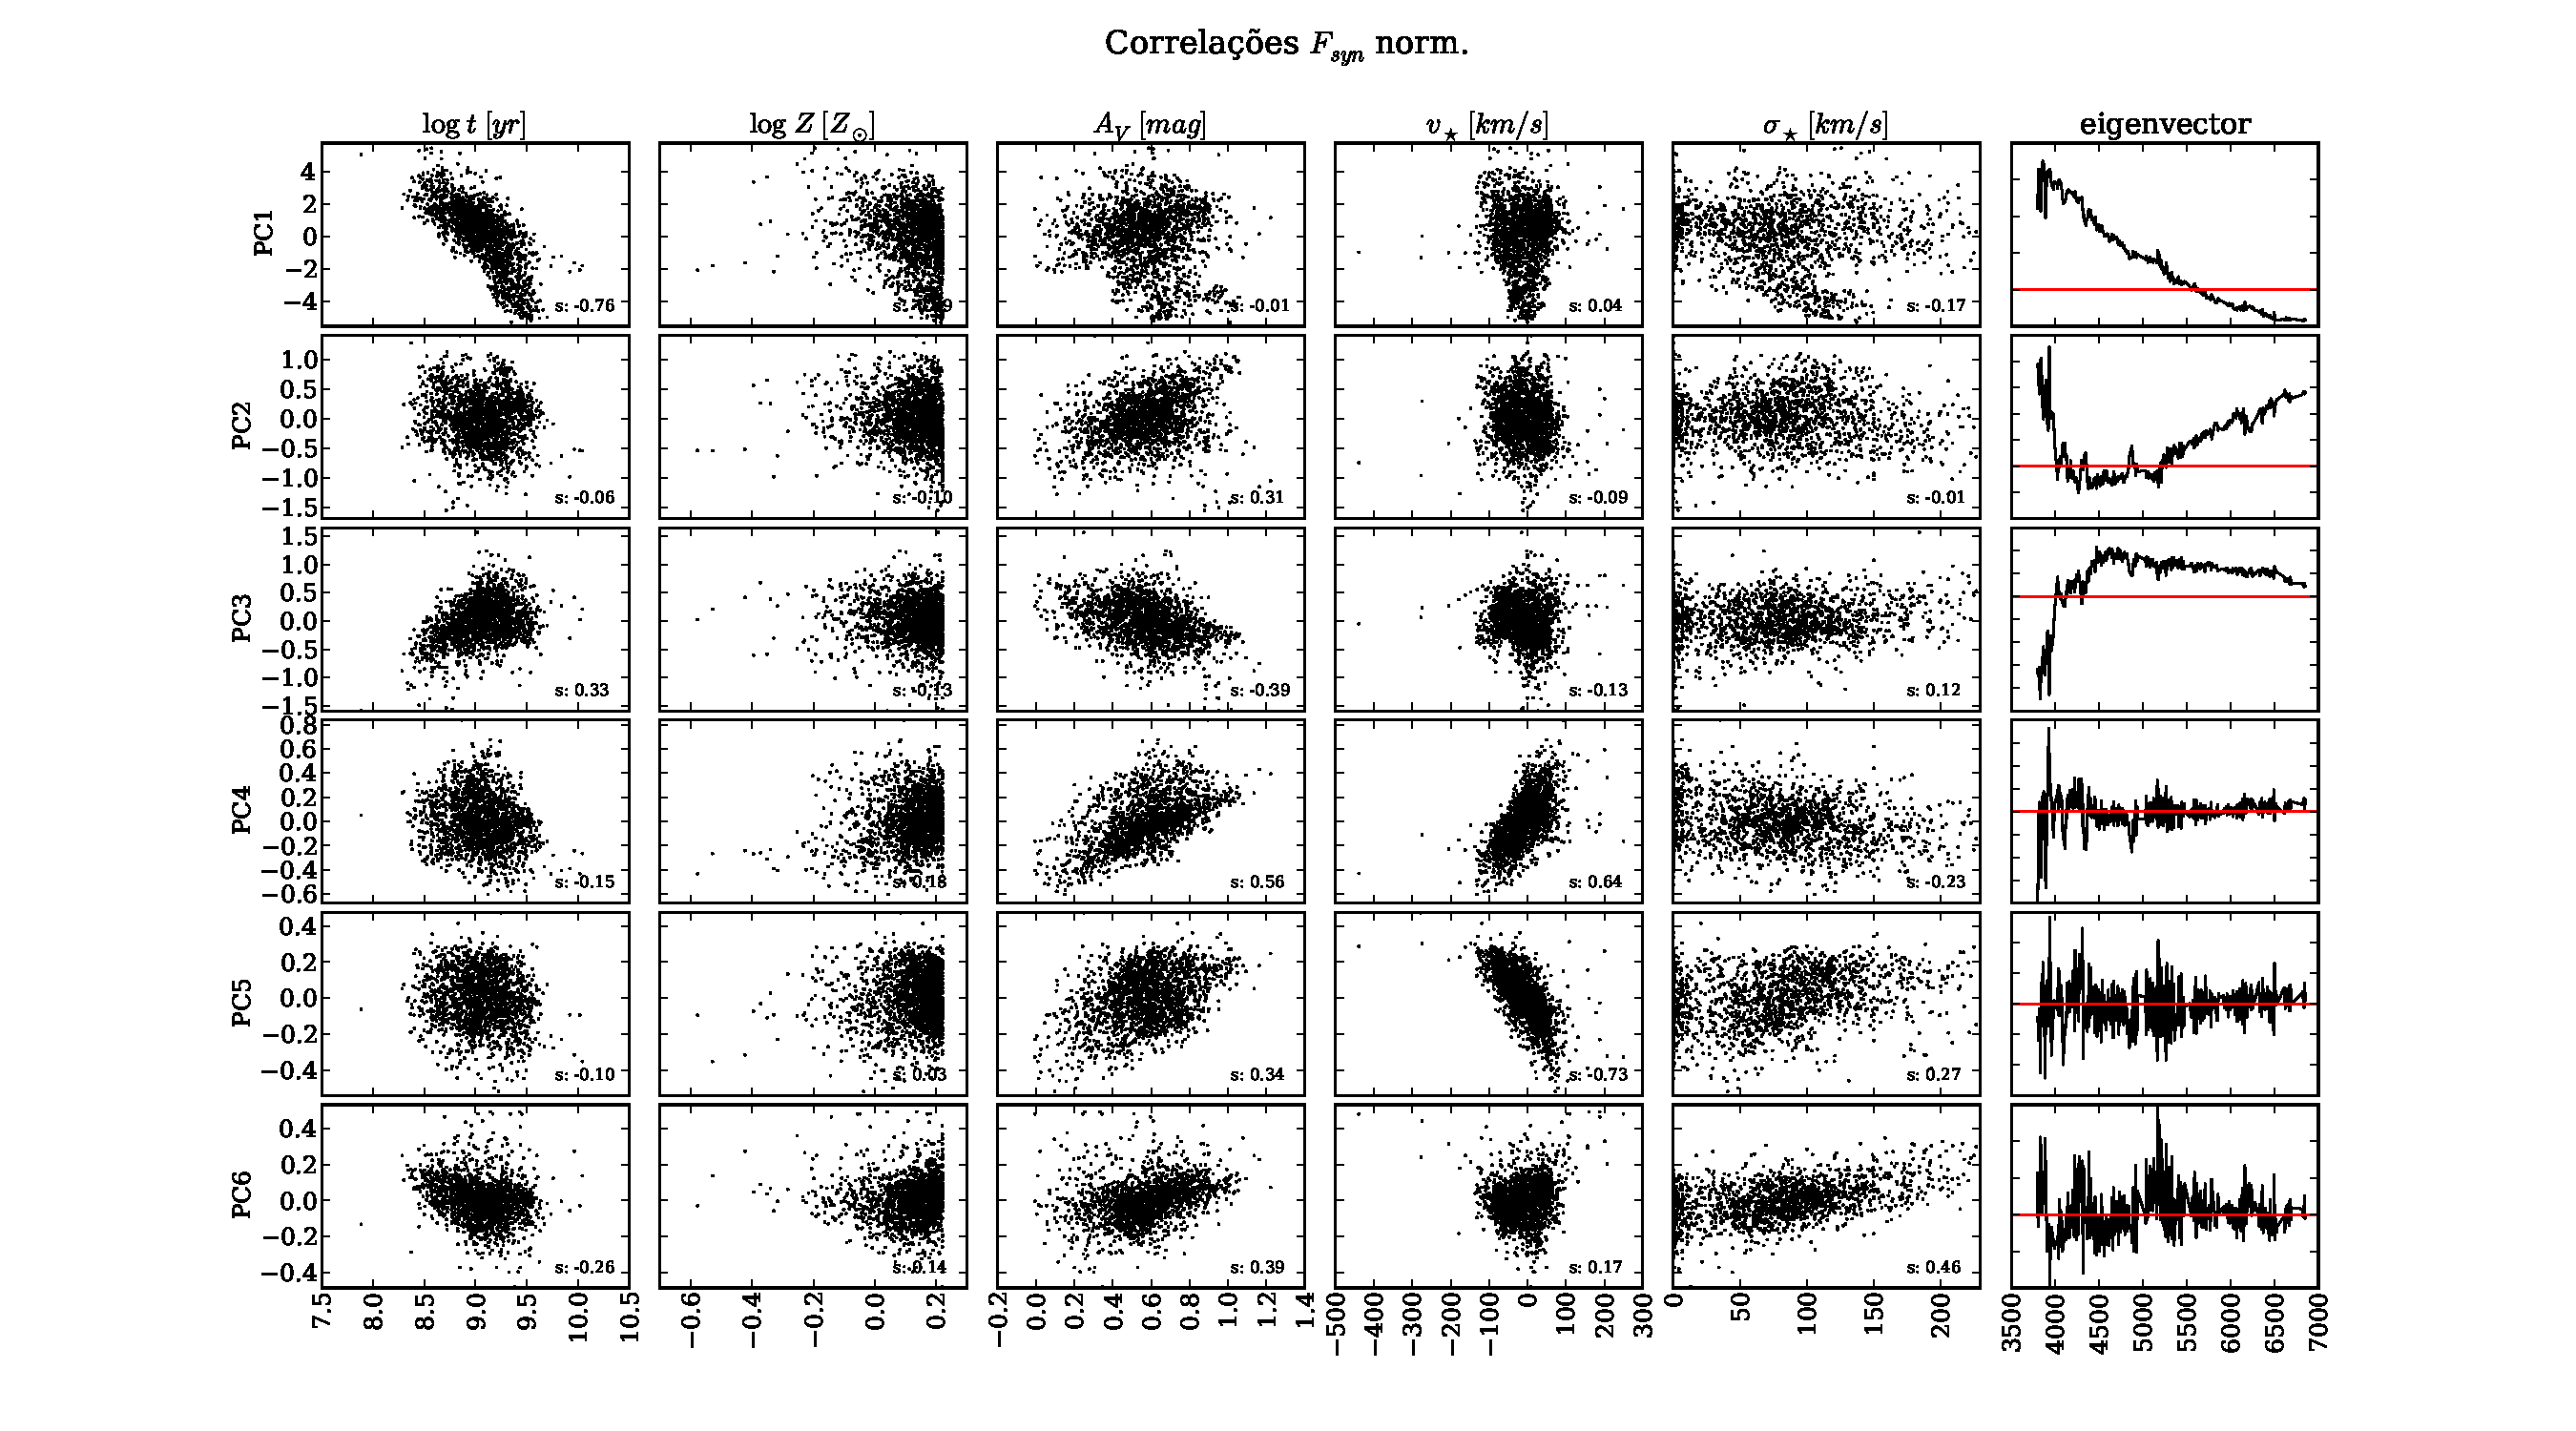
\includegraphics[width=1.3\textwidth, angle=-90]{figuras/K0073-correl-f_syn_norm-PCvsPhys.pdf}
	\caption[Correlações PCs vs. par\^ametros f\'isicos - $F_{syn}$ norm. - NGC 0001]
	{Igual a Figura \ref{fig:K0008correfsynnorm} para a galáxia NGC 0776.}
    \label{fig:K0073correfsynnorm}
\end{figure}

\subsection{NGC 4210 - CALIFA 518}

\begin{figure}
    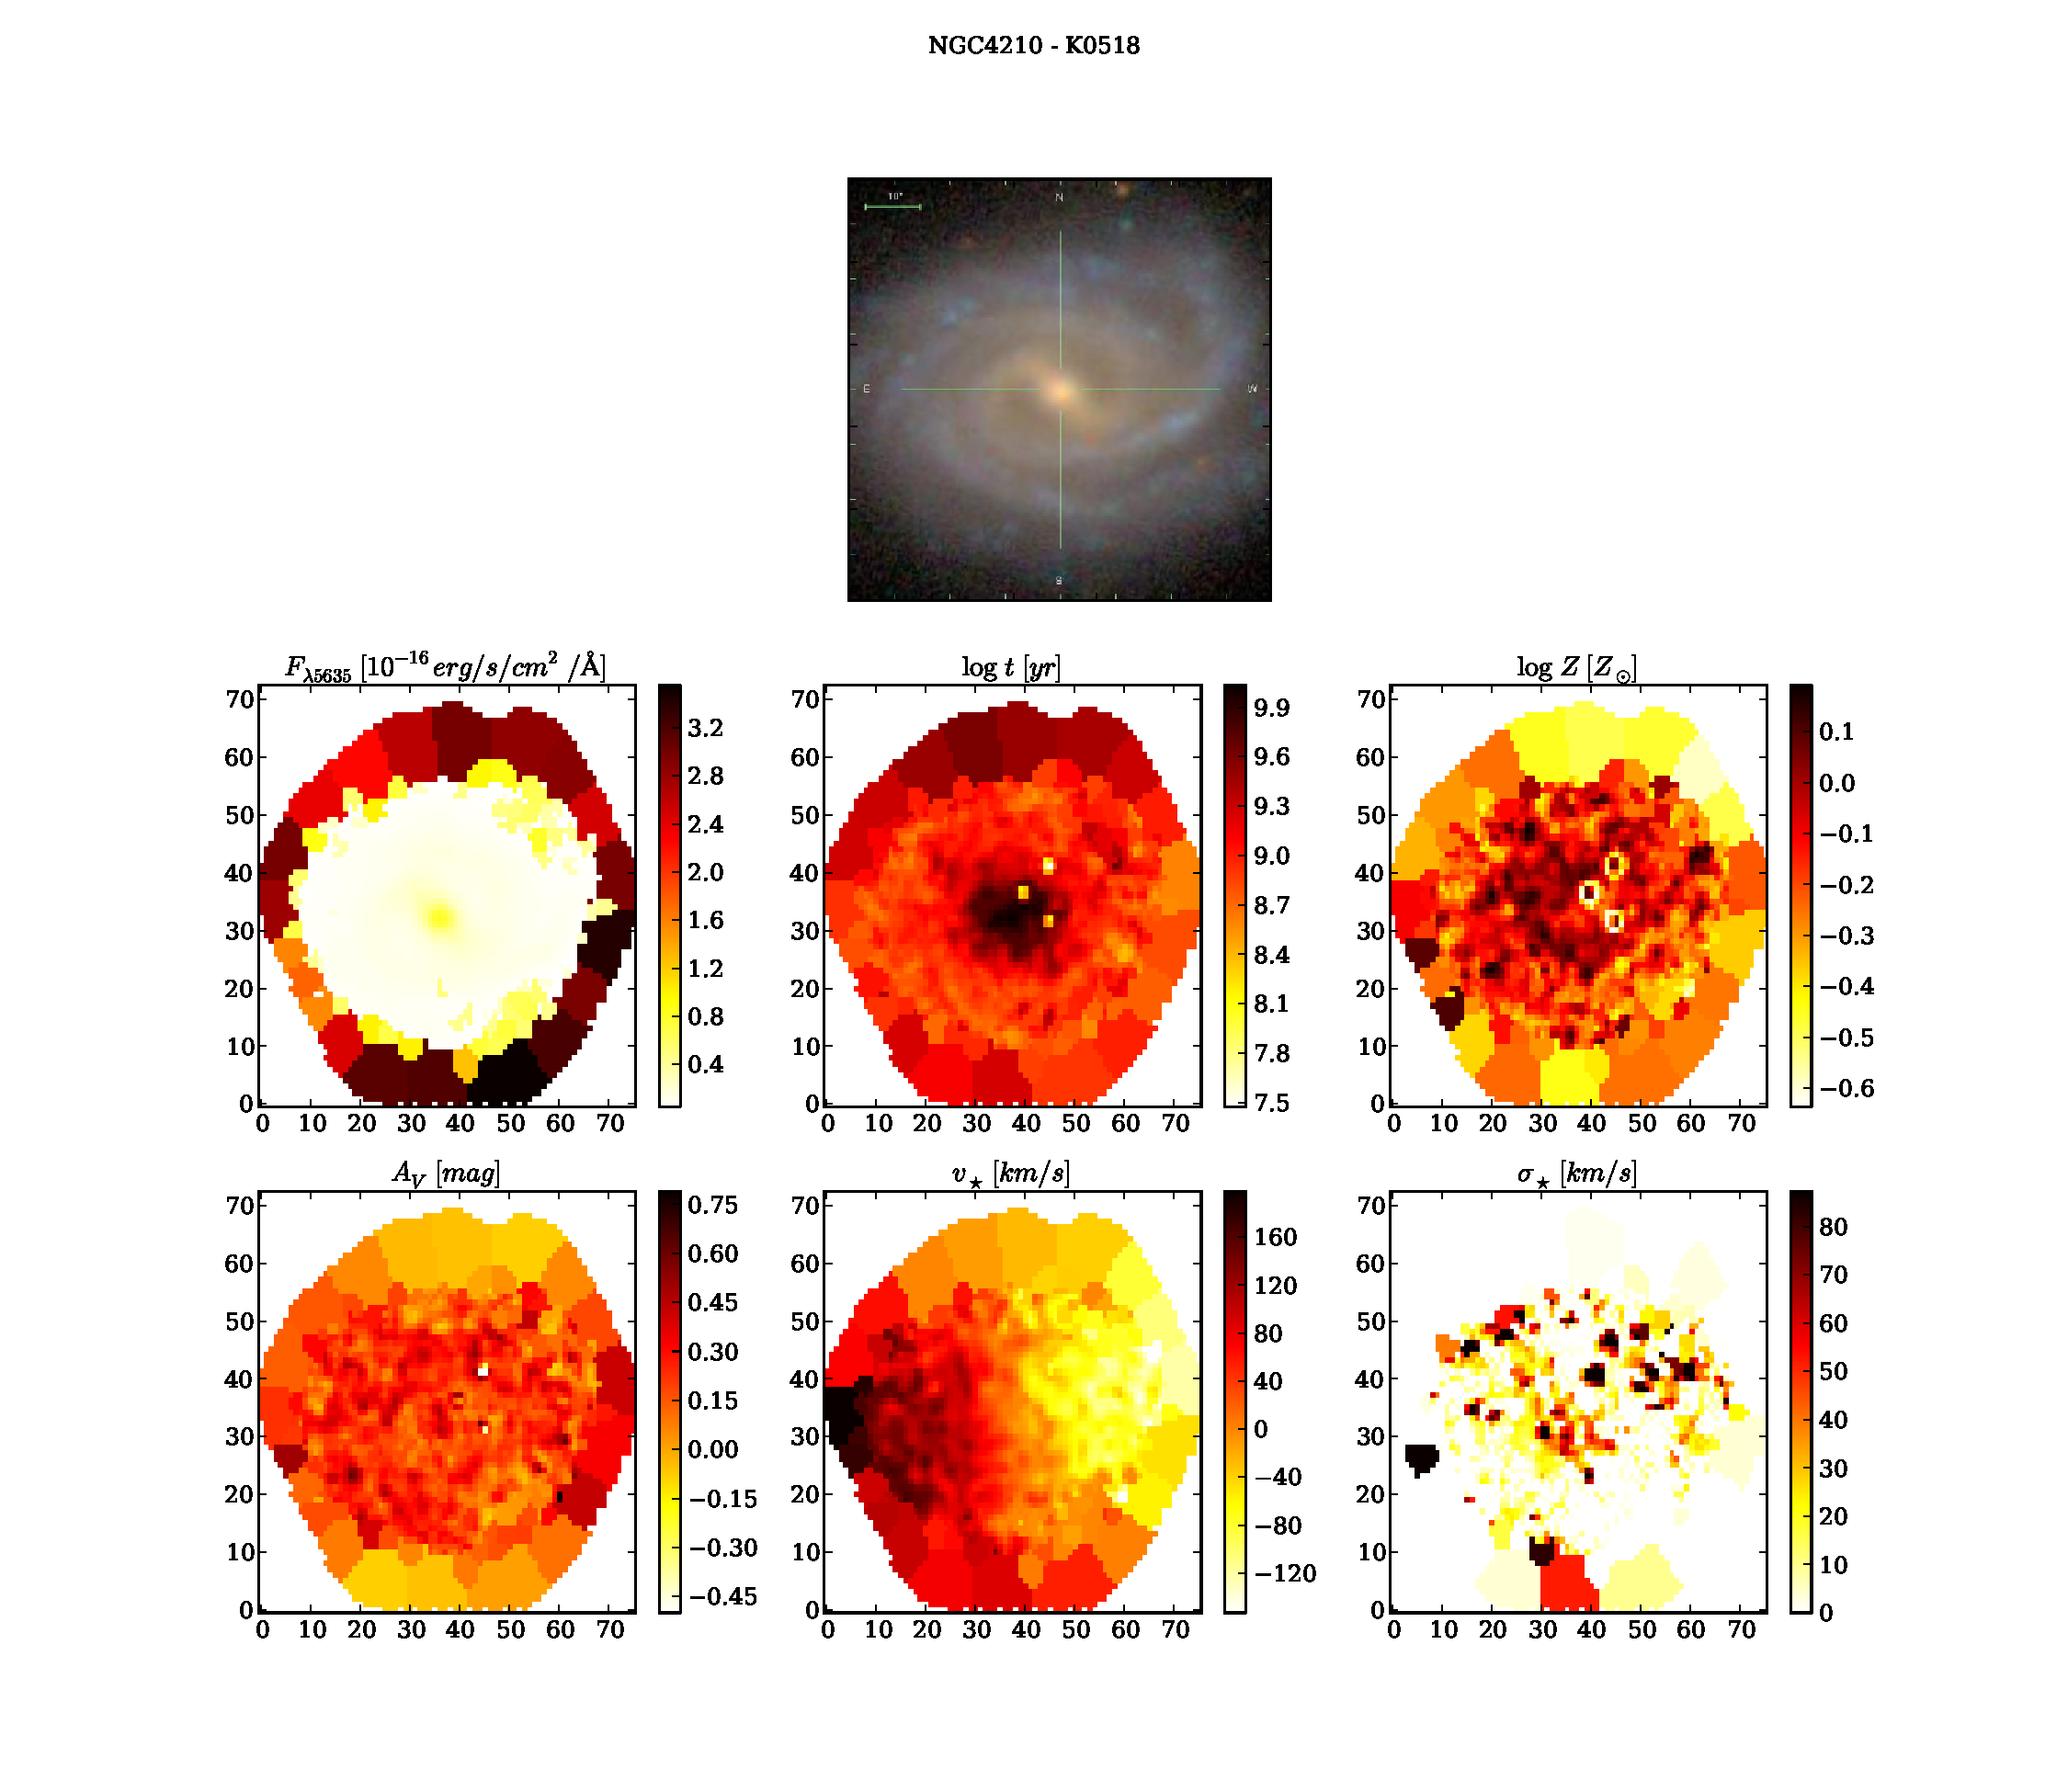
\includegraphics[width=1.\textwidth]{figuras/K0518-apresent.pdf}
    \caption[Propriedades f\'isicas da gal\'axia NGC 4210.]
    {Igual a Figura \ref{fig:K0008apresent} para a galáxia NGC 4210.}
    \label{fig:K0518apresent}
\end{figure}

\begin{figure}
    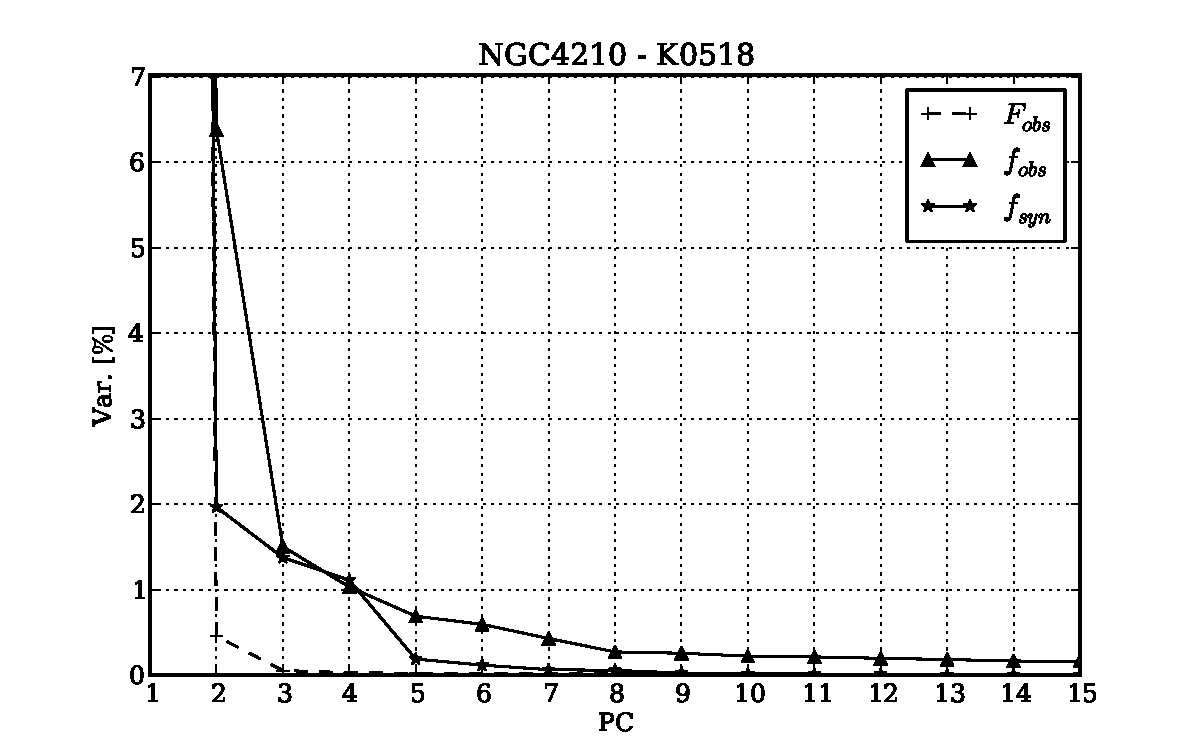
\includegraphics[height=0.33\textheight]{figuras/K0518-screetest.pdf}
    \caption[Scree test comparativo entre 3 PCAs - NGC 4210.]
	{Igual a Figura \ref{fig:K0008scree} para a galáxia NGC 4210.}
    \label{fig:K00518scree}
\end{figure}

\begin{figure}
    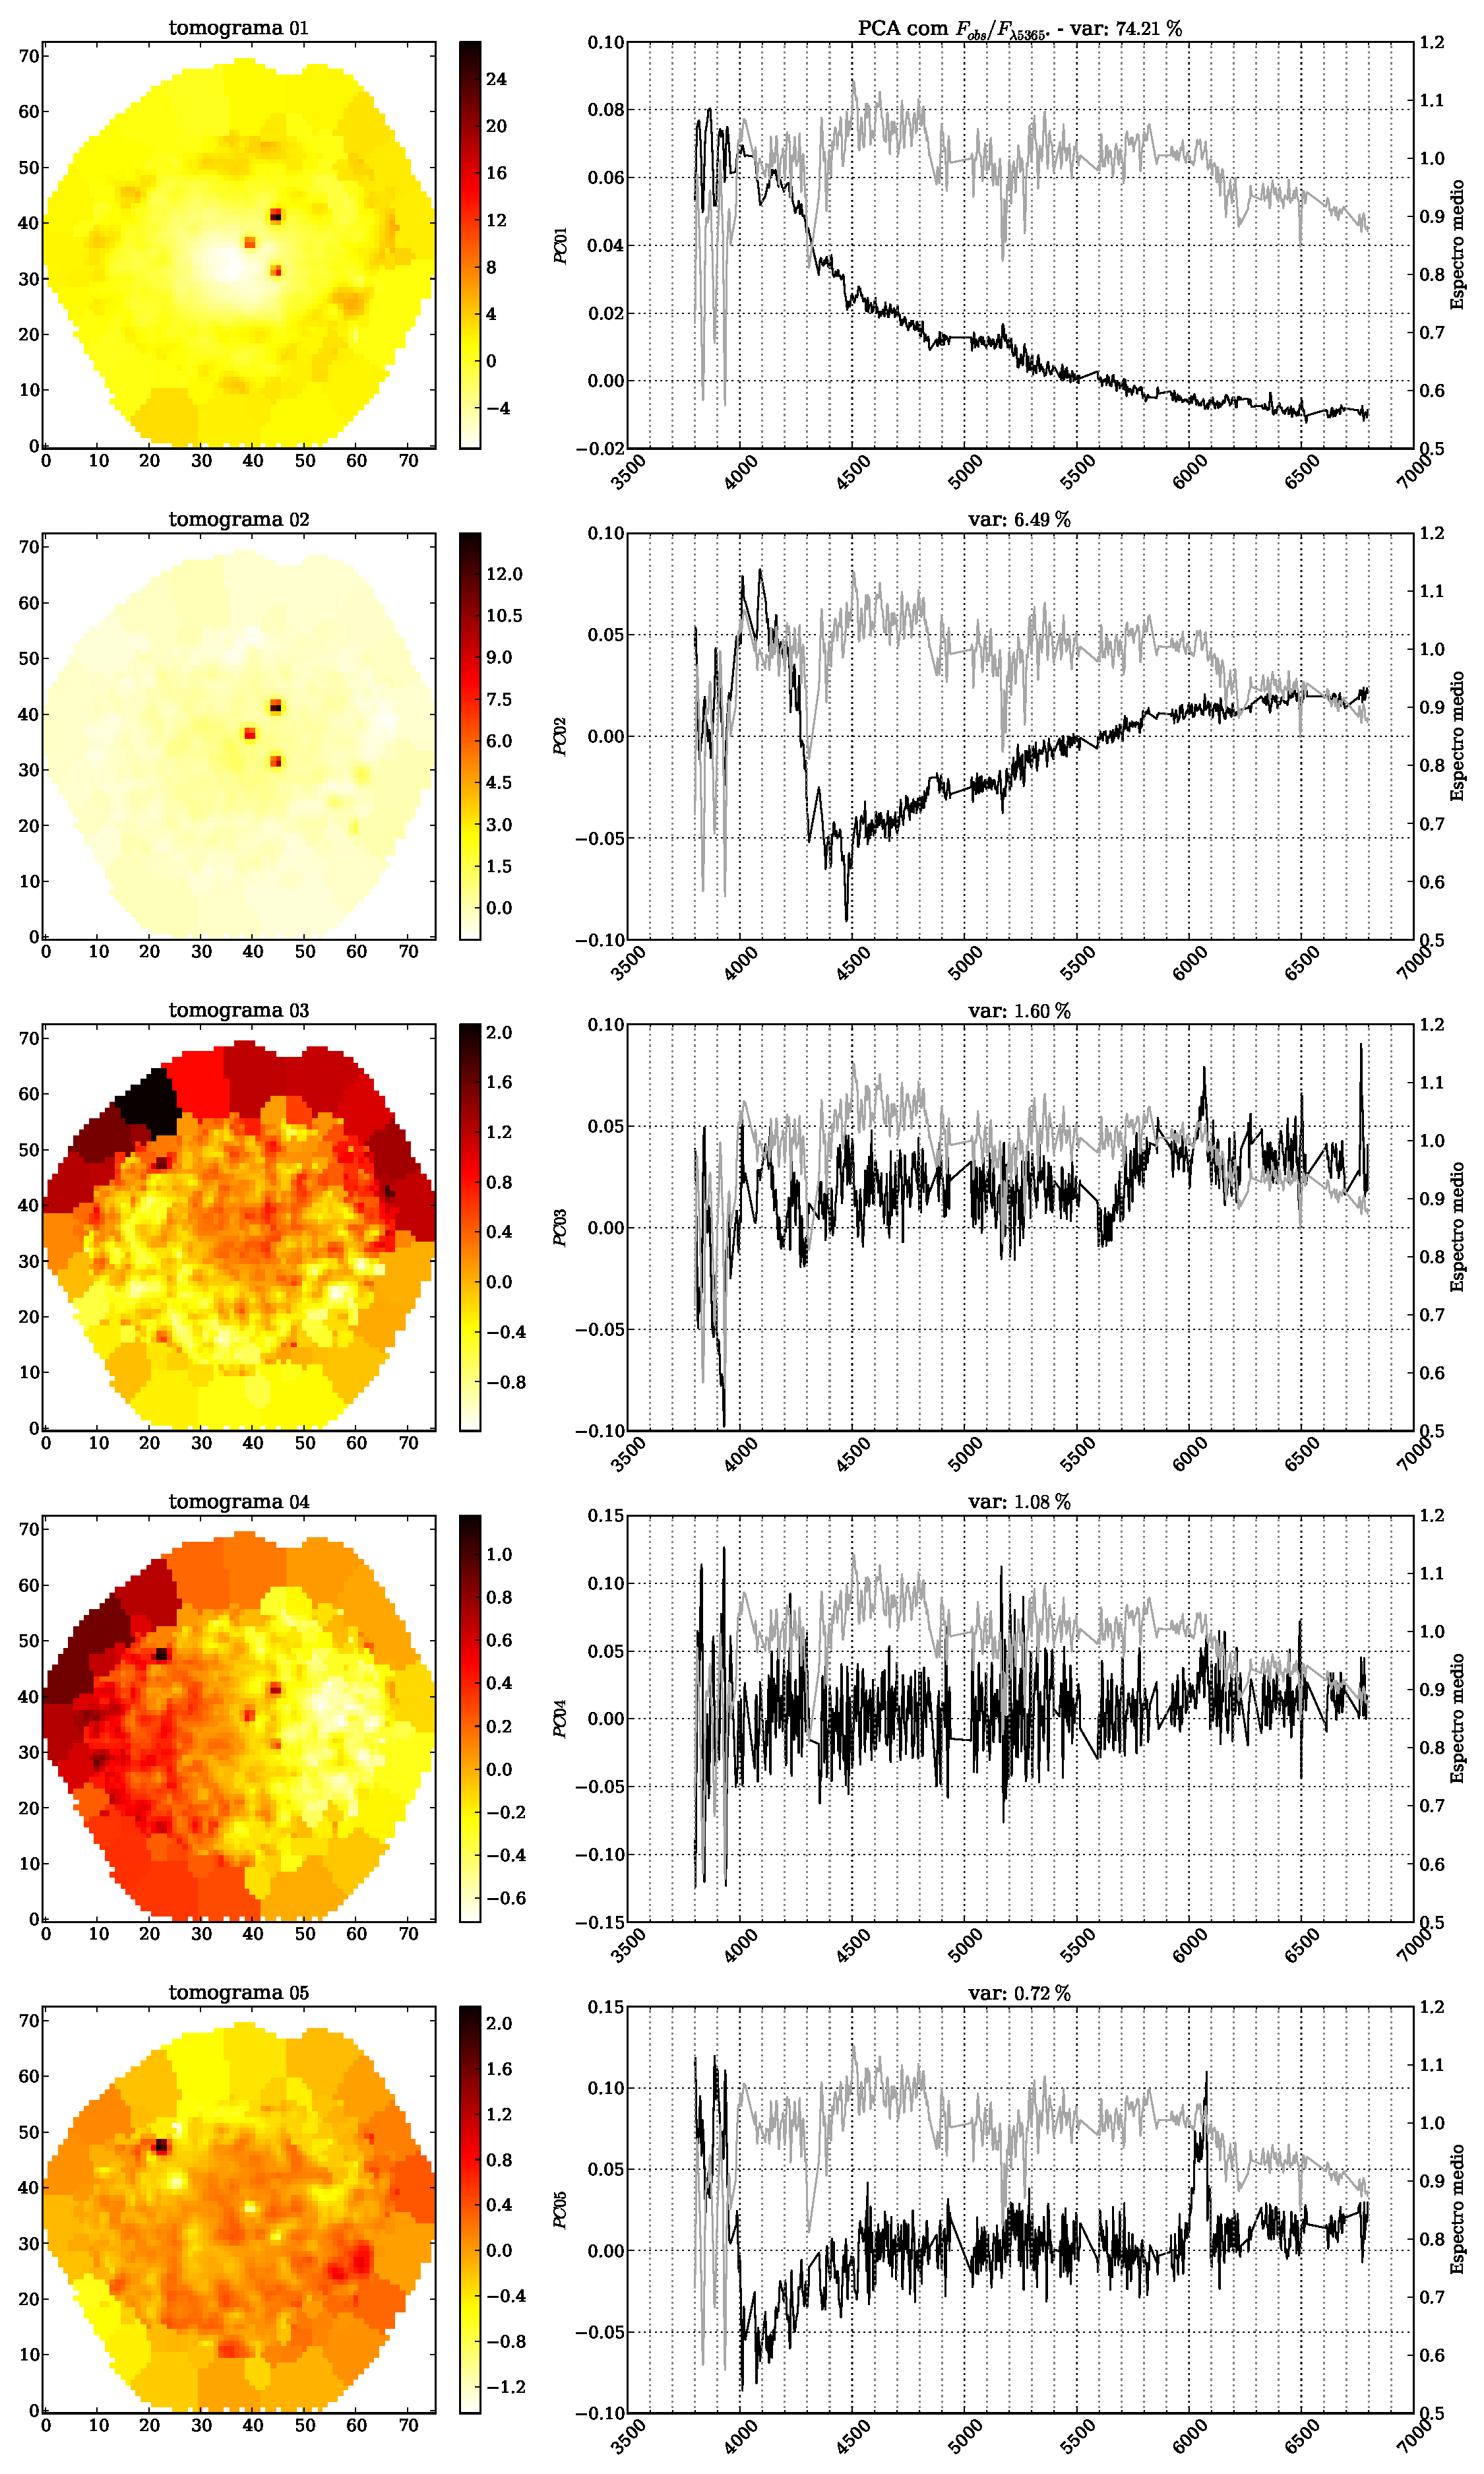
\includegraphics[width=0.85\textwidth]{figuras/K0518-tomo-obs-norm.pdf}
    \caption[Tomogramas de 1 a 5 para o cubo $F_{obs}$ norm. - NGC 4210.]
    {Igual a Figura \ref{fig:K0008tomofobsnorm} para a galáxia NGC 4210.}
    \label{fig:K0518tomofobsnorm}
\end{figure}

\begin{figure}
    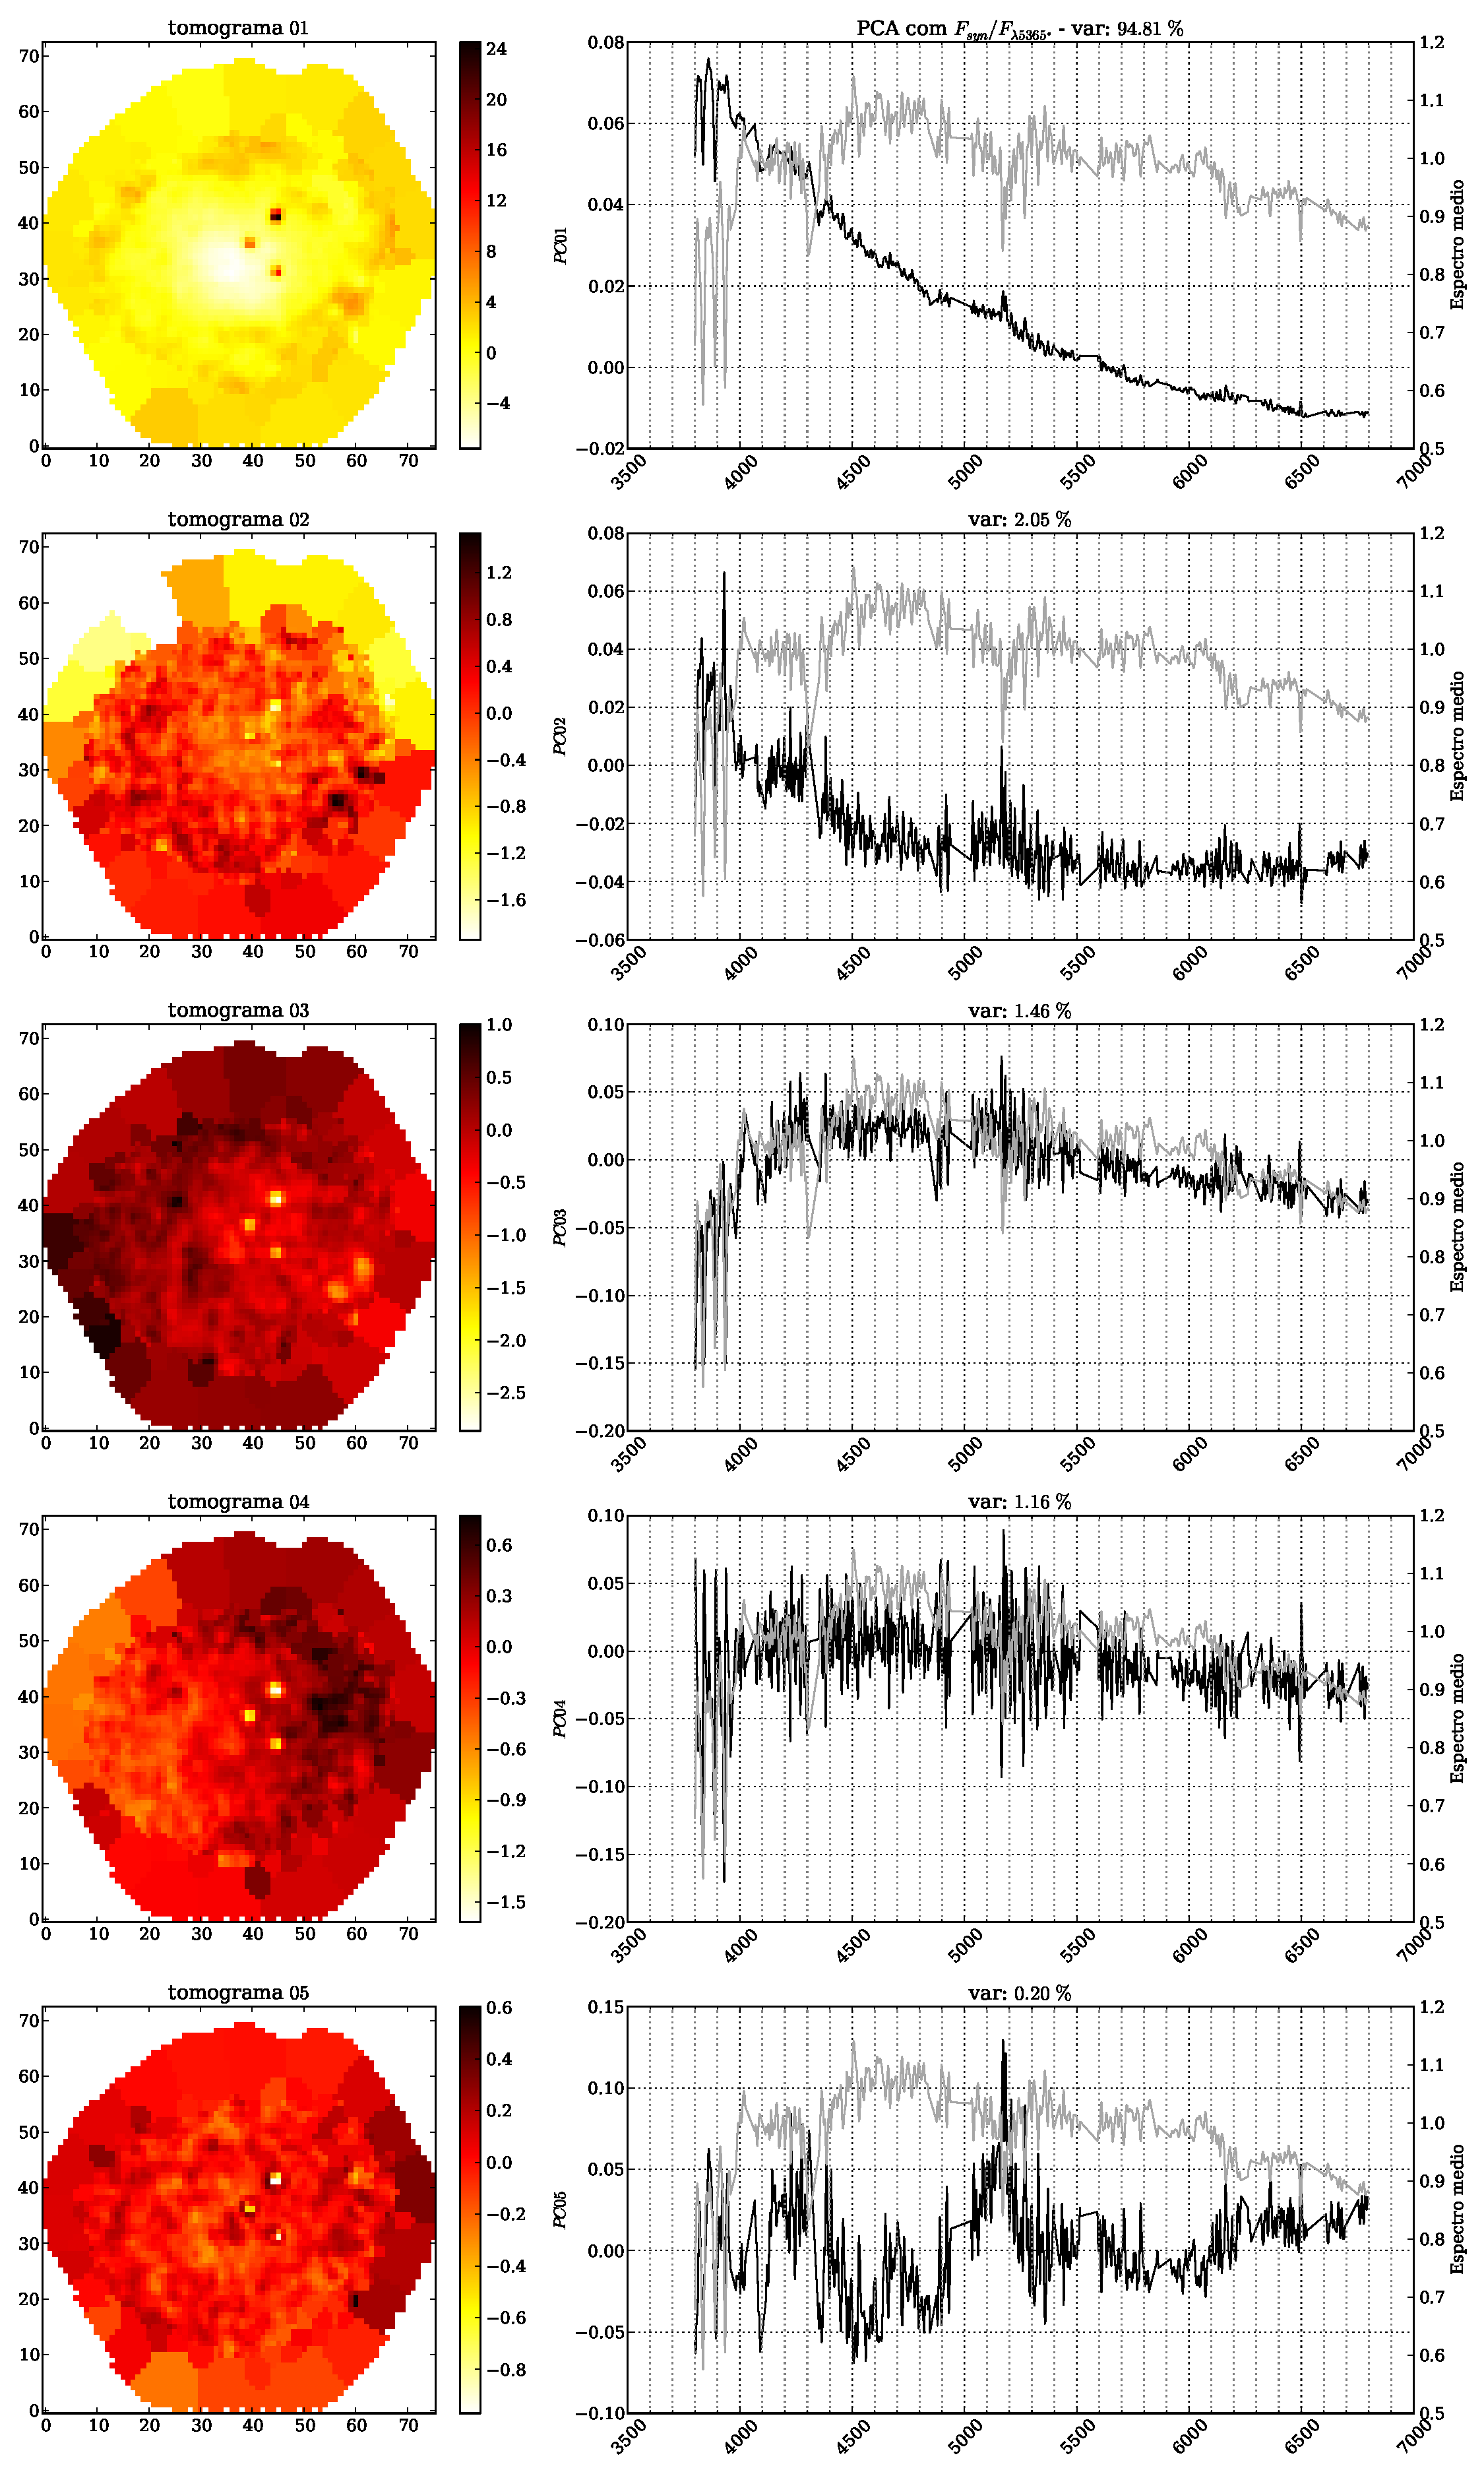
\includegraphics[width=0.85\textwidth]{figuras/K0518-tomo-syn-norm.pdf}
    \caption[Tomogramas de 1 a 5 para o cubo $F_{syn}$ norm. - NGC 4210.]
    {Igual a Figura \ref{fig:K0008tomofsynnorm} para a galáxia NGC 4210.}
    \label{fig:K0518tomofsynnorm}
\end{figure}

\begin{figure}
    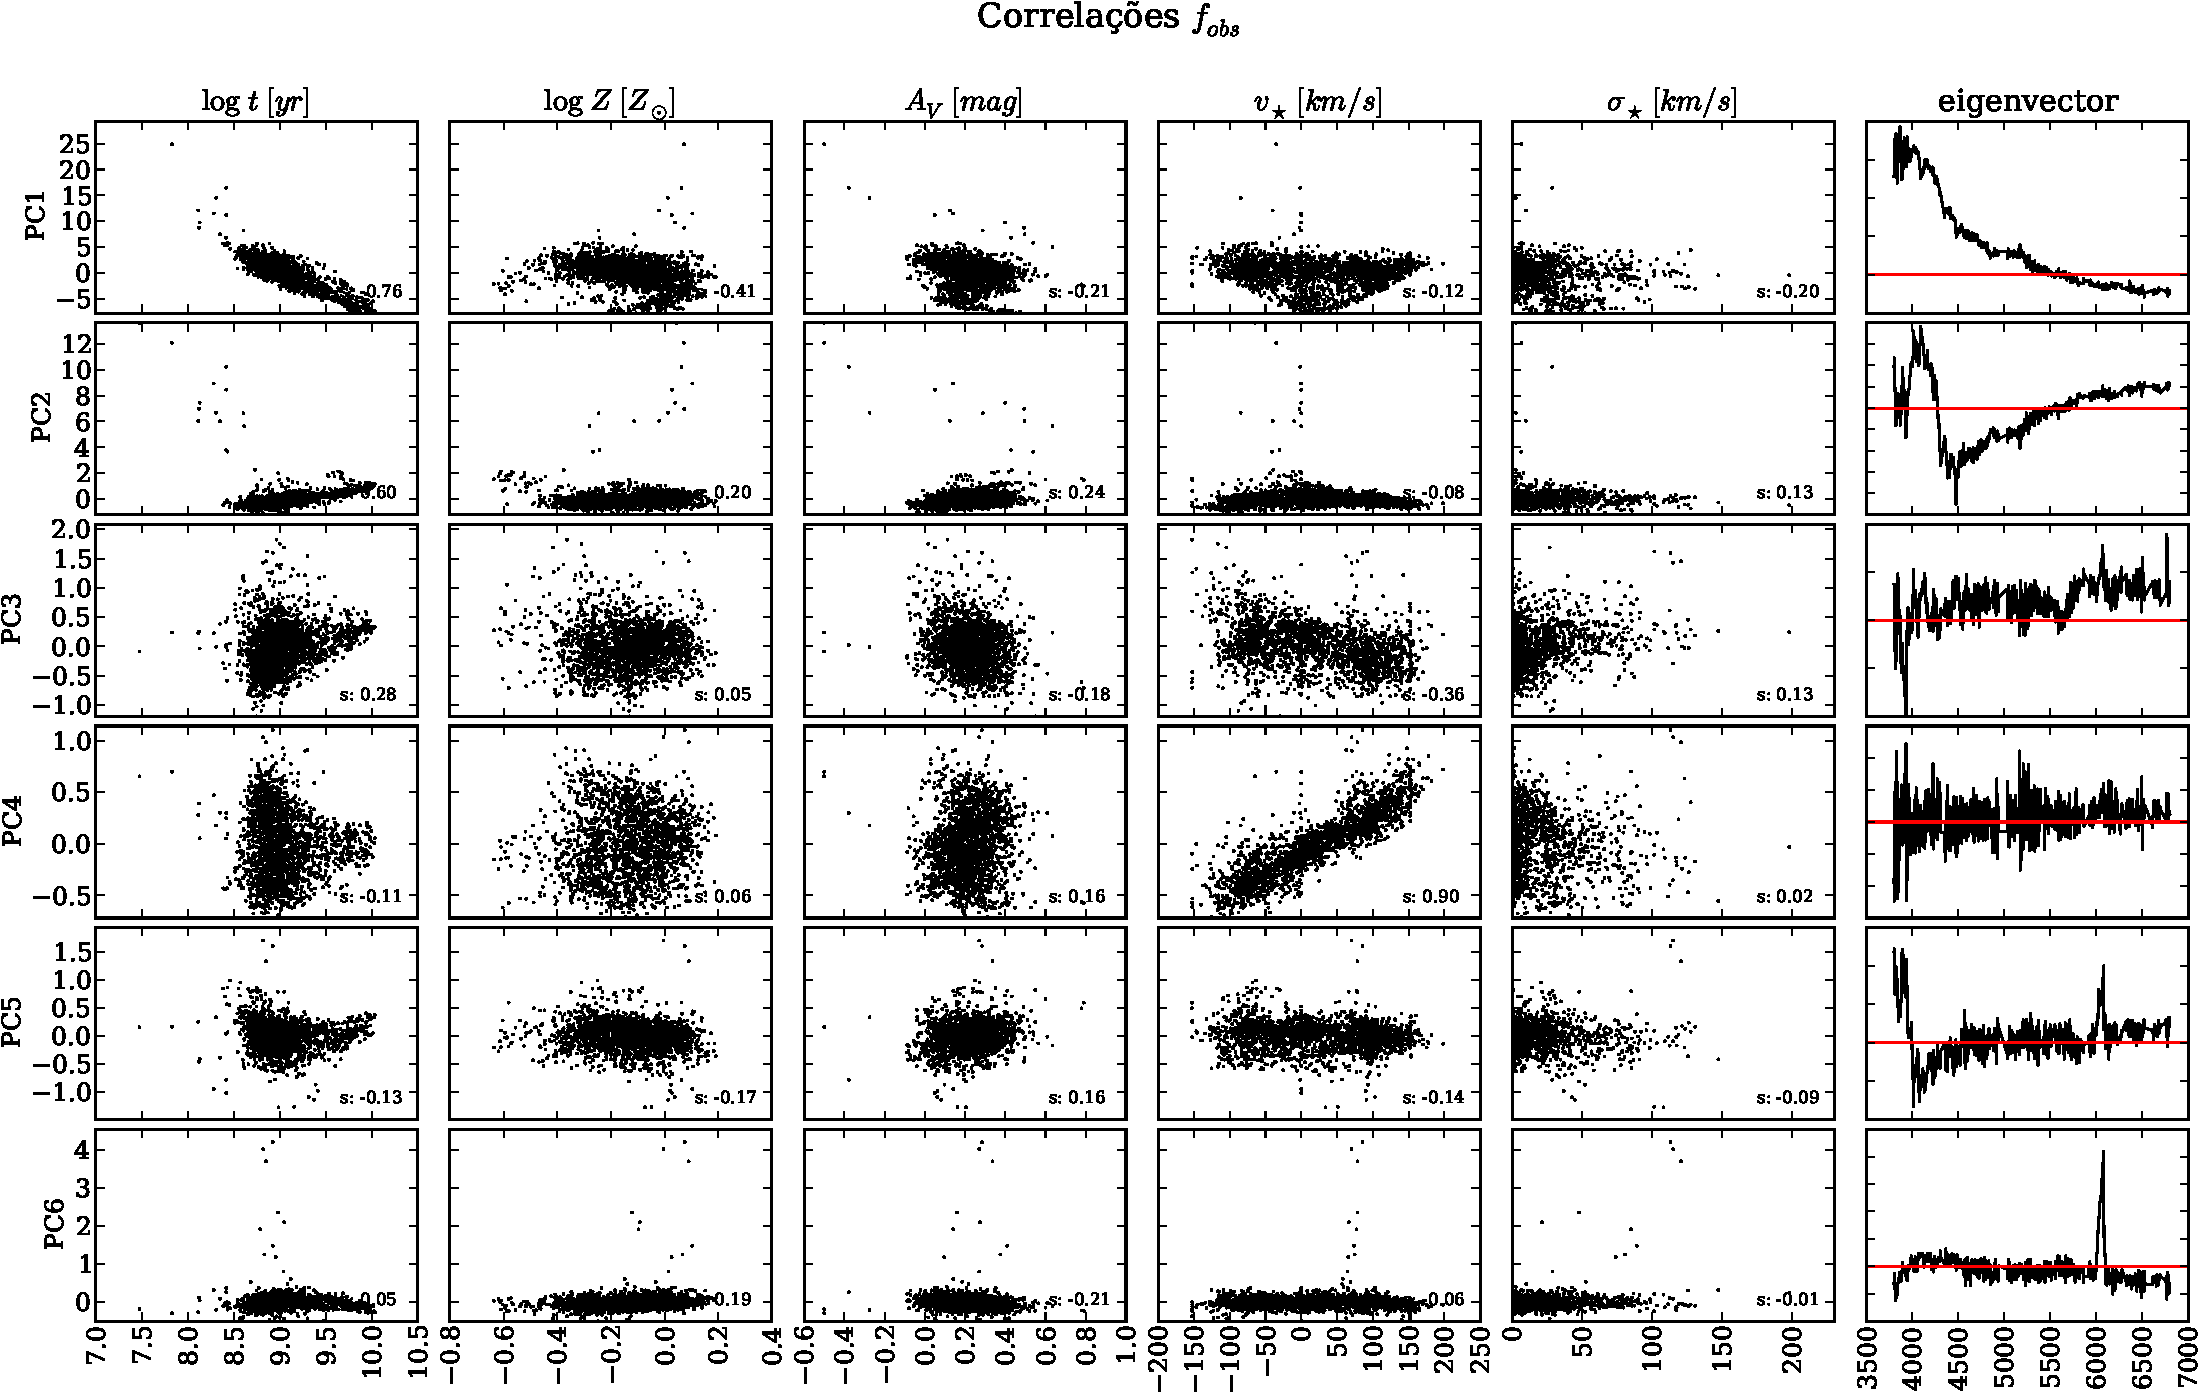
\includegraphics[width=1.3\textwidth, angle=-90]{figuras/K0518-correl-f_obs_norm-PCvsPhys.pdf}
	\caption[Correlações PCs vs. par\^ametros f\'isicos - $F_{obs}$ norm. - NGC 4210.]
	{Igual a Figura \ref{fig:K0008correfobsnorm} para a galáxia NGC 4210.}
    \label{fig:K0518correfobsnorm}
\end{figure}

\begin{figure}
    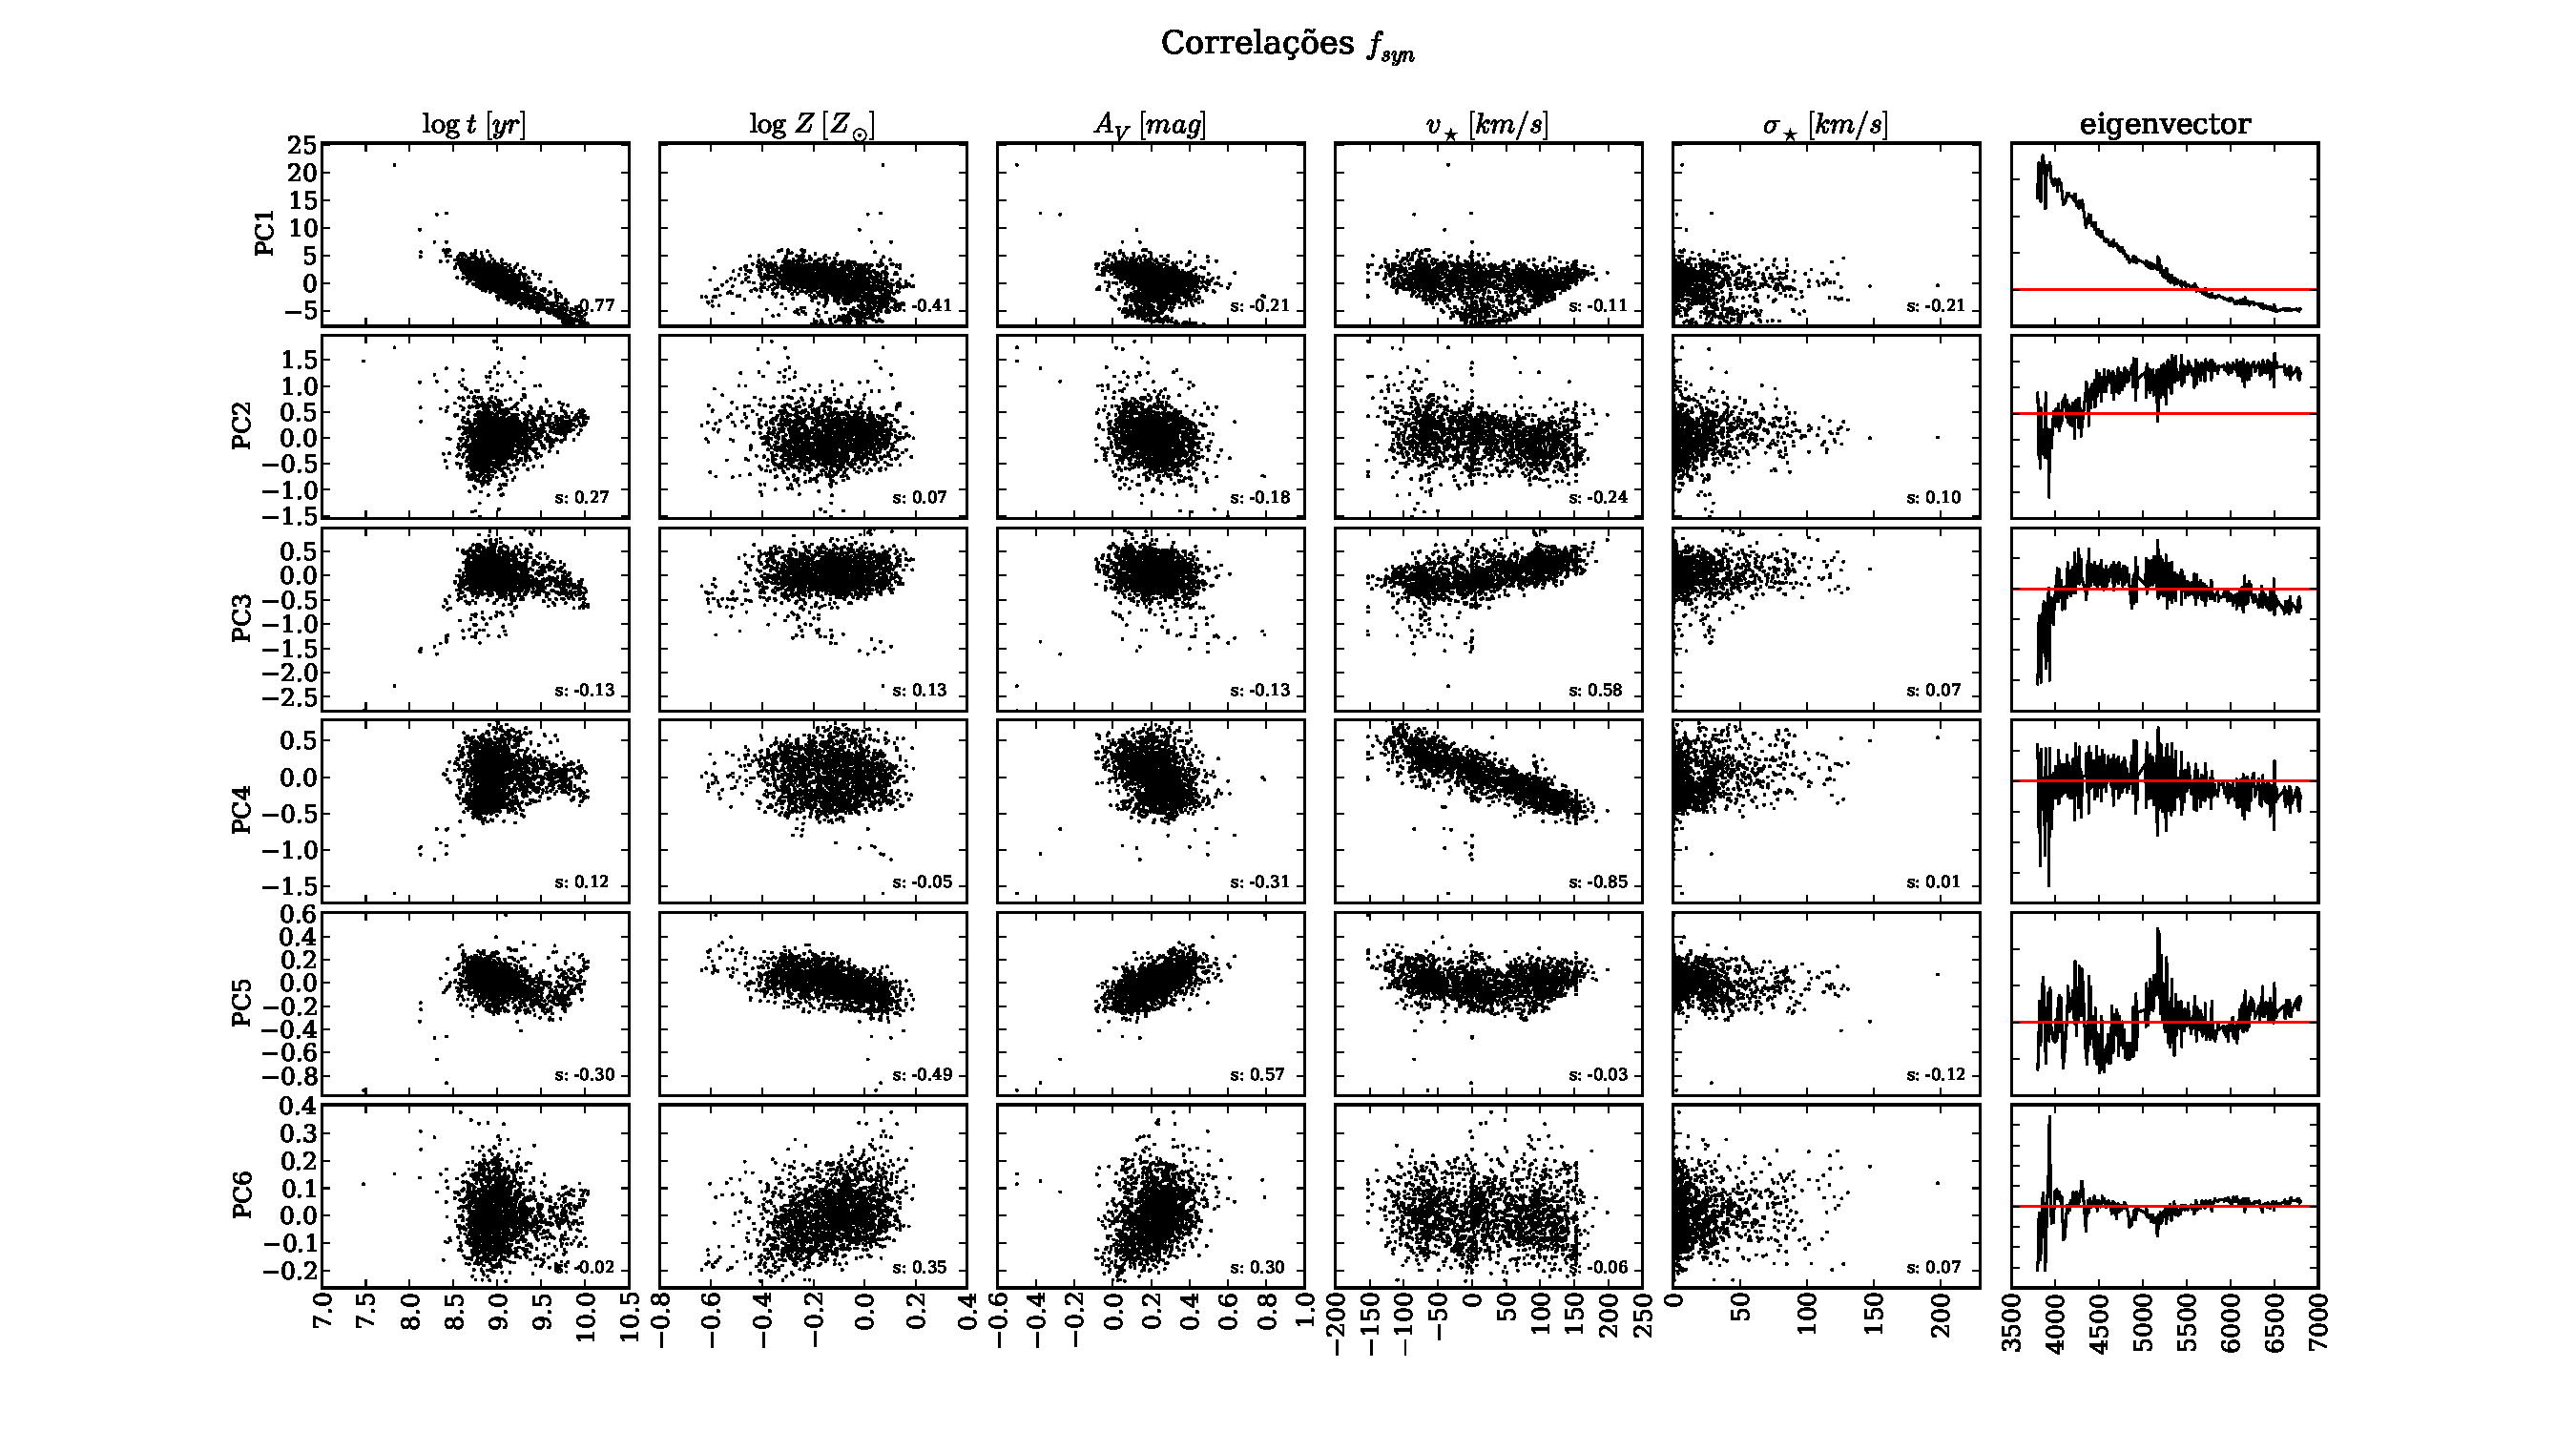
\includegraphics[width=1.3\textwidth, angle=-90]{figuras/K0518-correl-f_syn_norm-PCvsPhys.pdf}
	\caption[Correlações PCs vs. par\^ametros f\'isicos - $F_{syn}$ norm. - NGC 4210.]
	{Igual a Figura \ref{fig:K0008correfsynnorm} para a galáxia NGC 4210.}
    \label{fig:K0518correfsynnorm}
\end{figure}

\section{Gal\'axias el\'ipticas}
\ref{sec:result:elipt}

\subsection{NGC 1167 - CALIFA 119}

\begin{figure}
    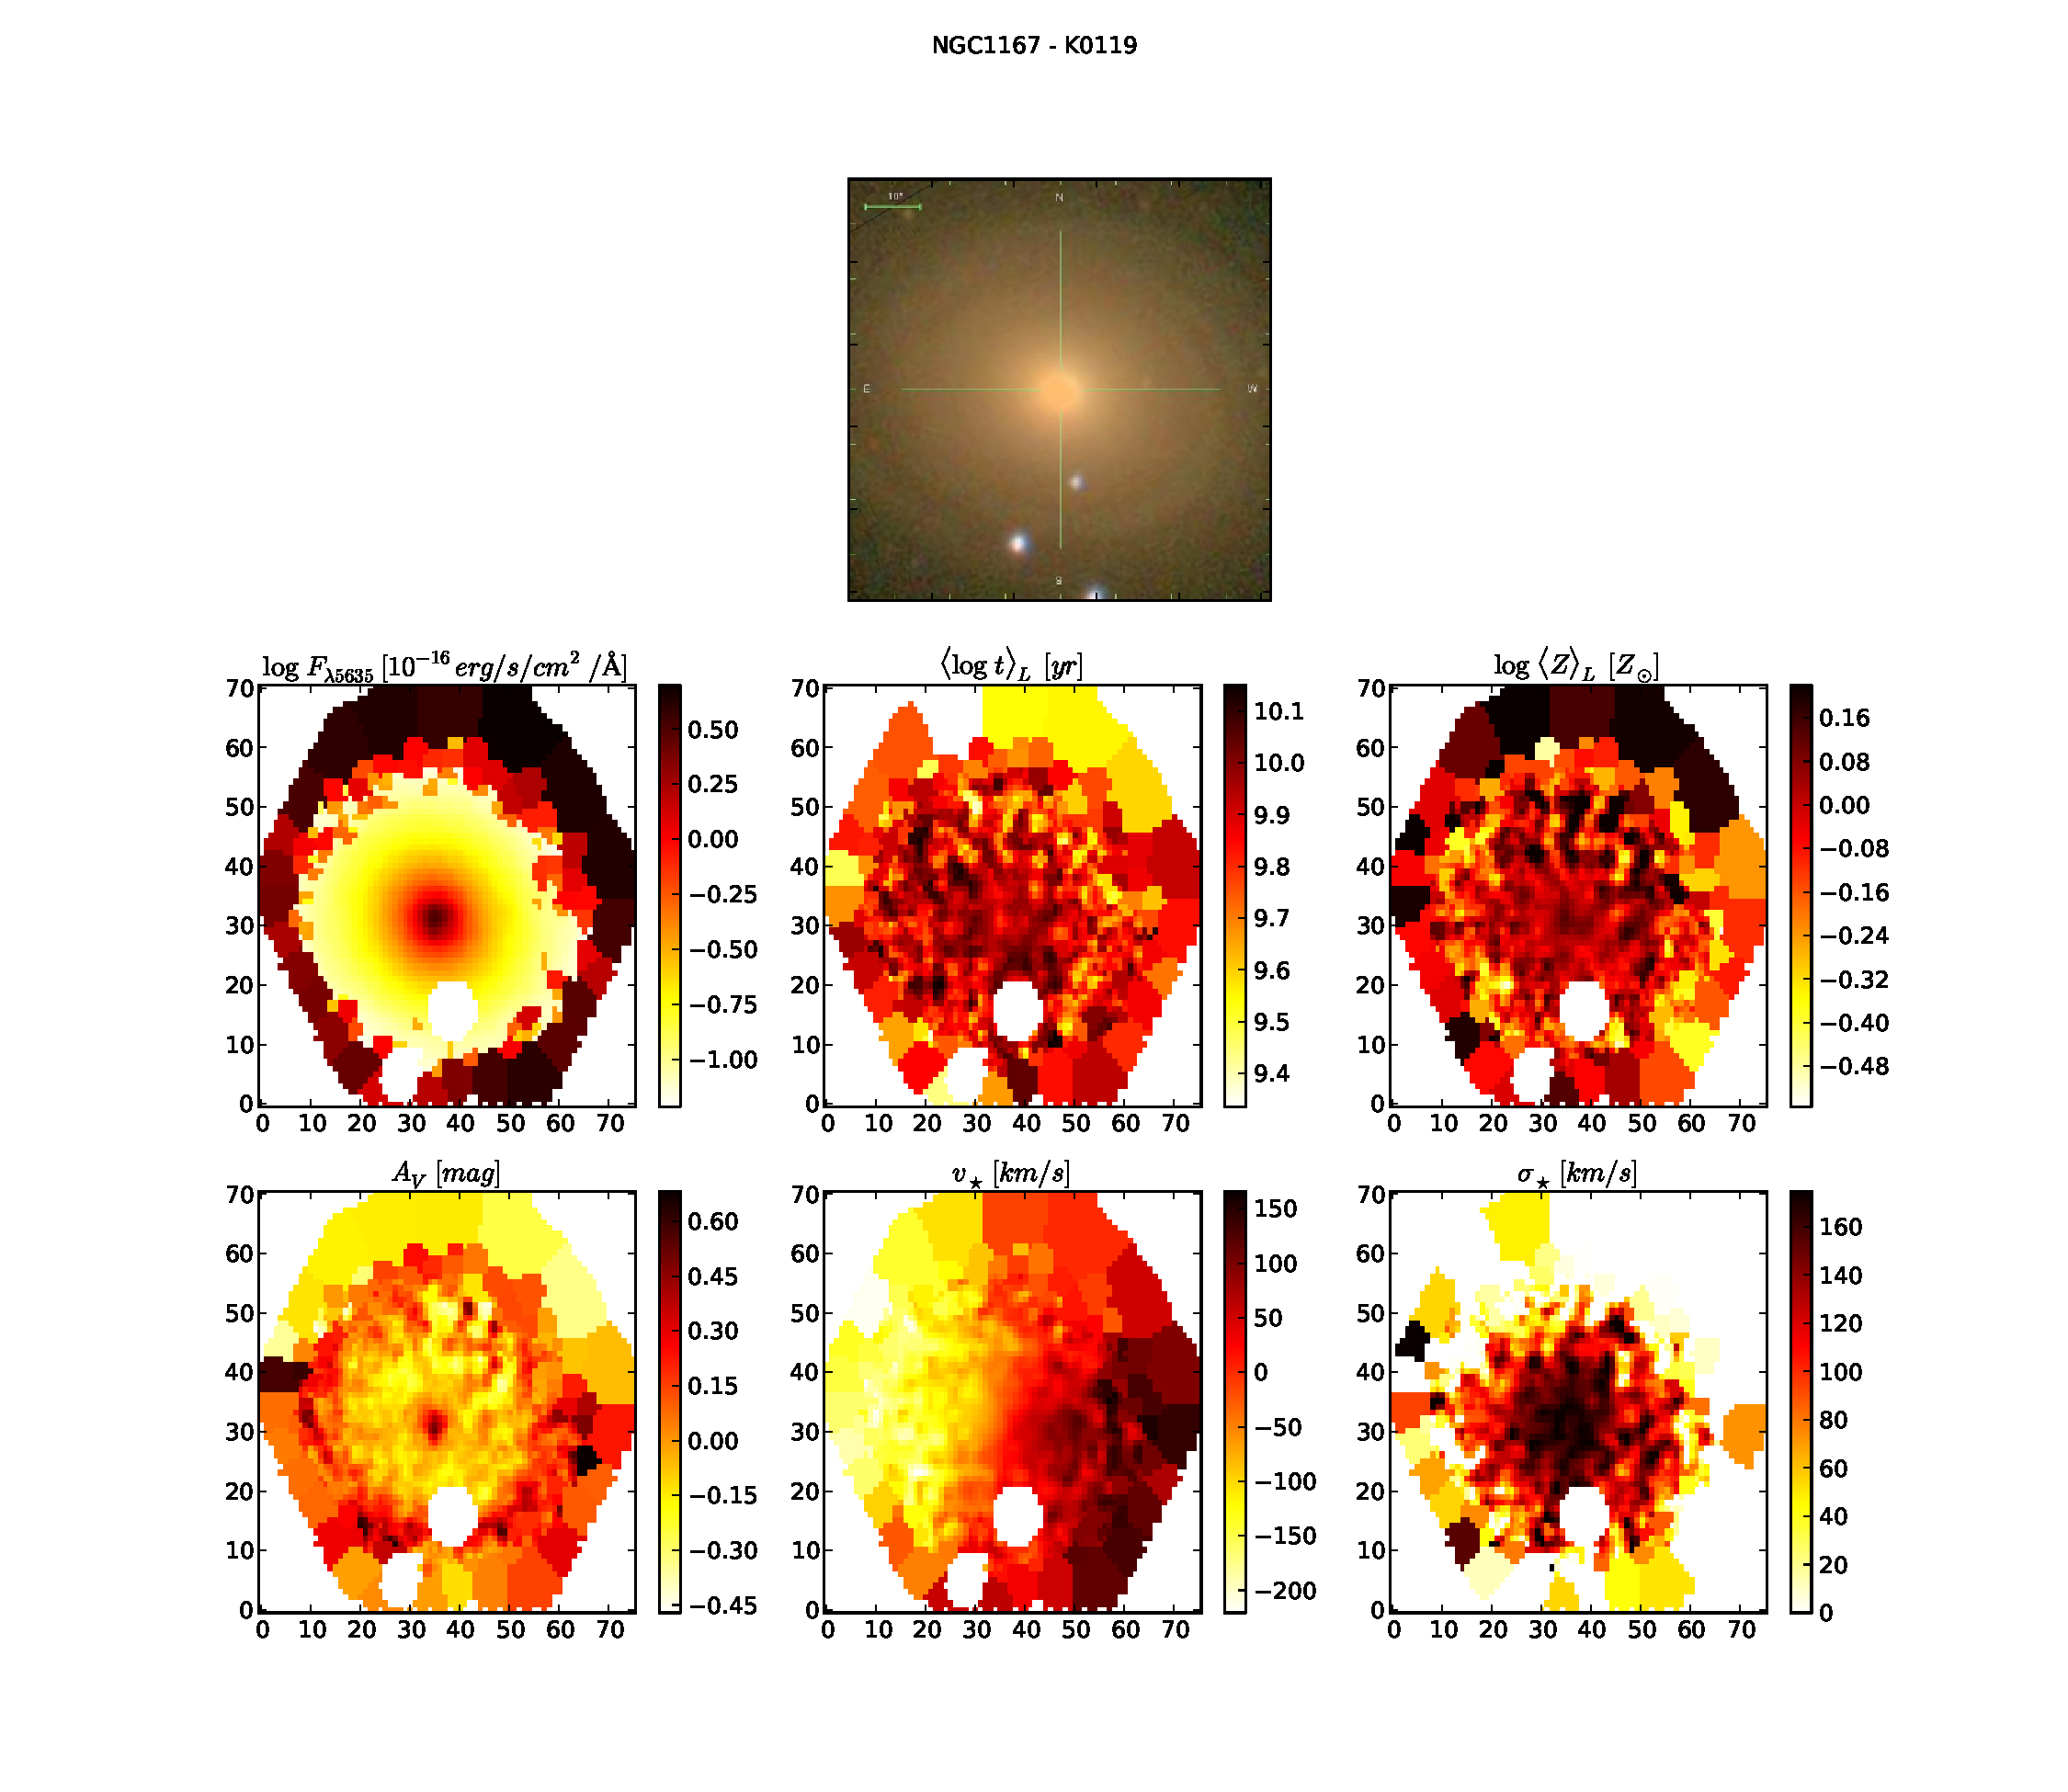
\includegraphics[width=1.\textwidth]{figuras/K0119-apresent.pdf}
    \caption[Propriedades f\'isicas da gal\'axia NGC 1167.]
    {Igual a Figura \ref{fig:K0008apresent} para a galáxia NGC 1167.}
    \label{fig:K0119apresent}
\end{figure}

\begin{figure}
    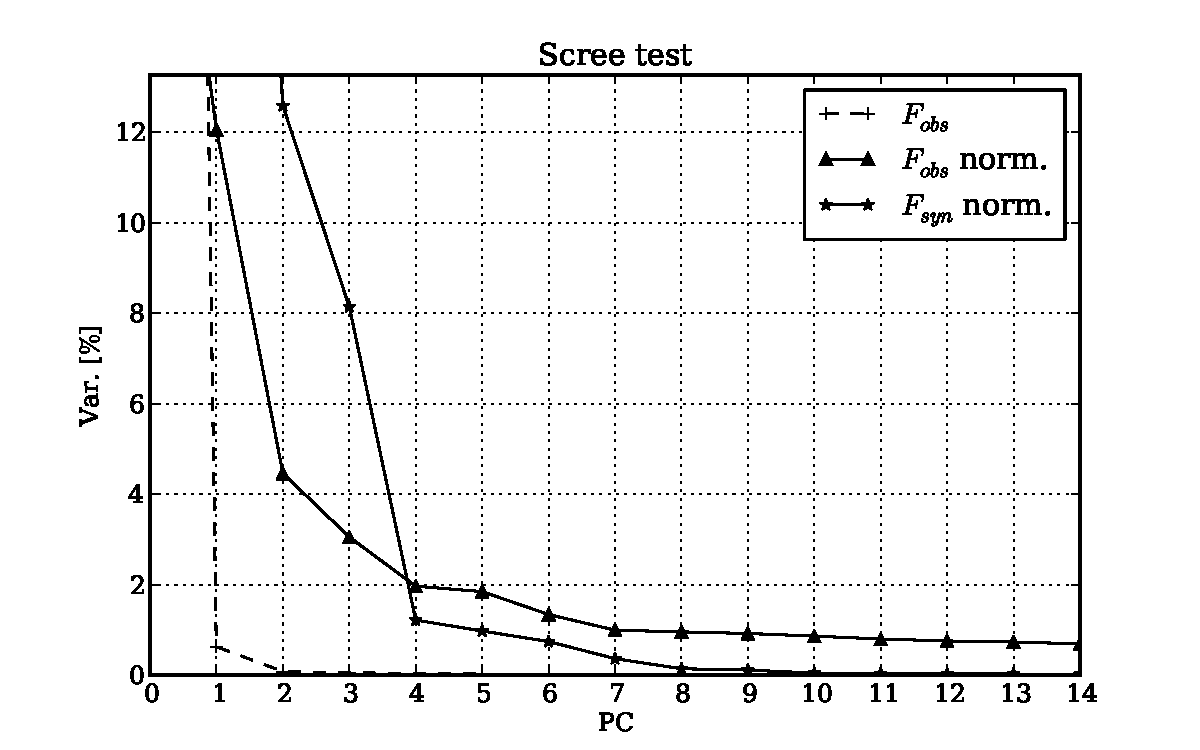
\includegraphics[height=0.33\textheight]{figuras/K0119-screetest.pdf}
    \caption[Scree test comparativo entre 3 PCAs - NGC 1167.]
    {Igual a Figura \ref{fig:K0008scree} para a galáxia NGC 1167.}
    \label{fig:K0119scree}
\end{figure}

\begin{figure}
    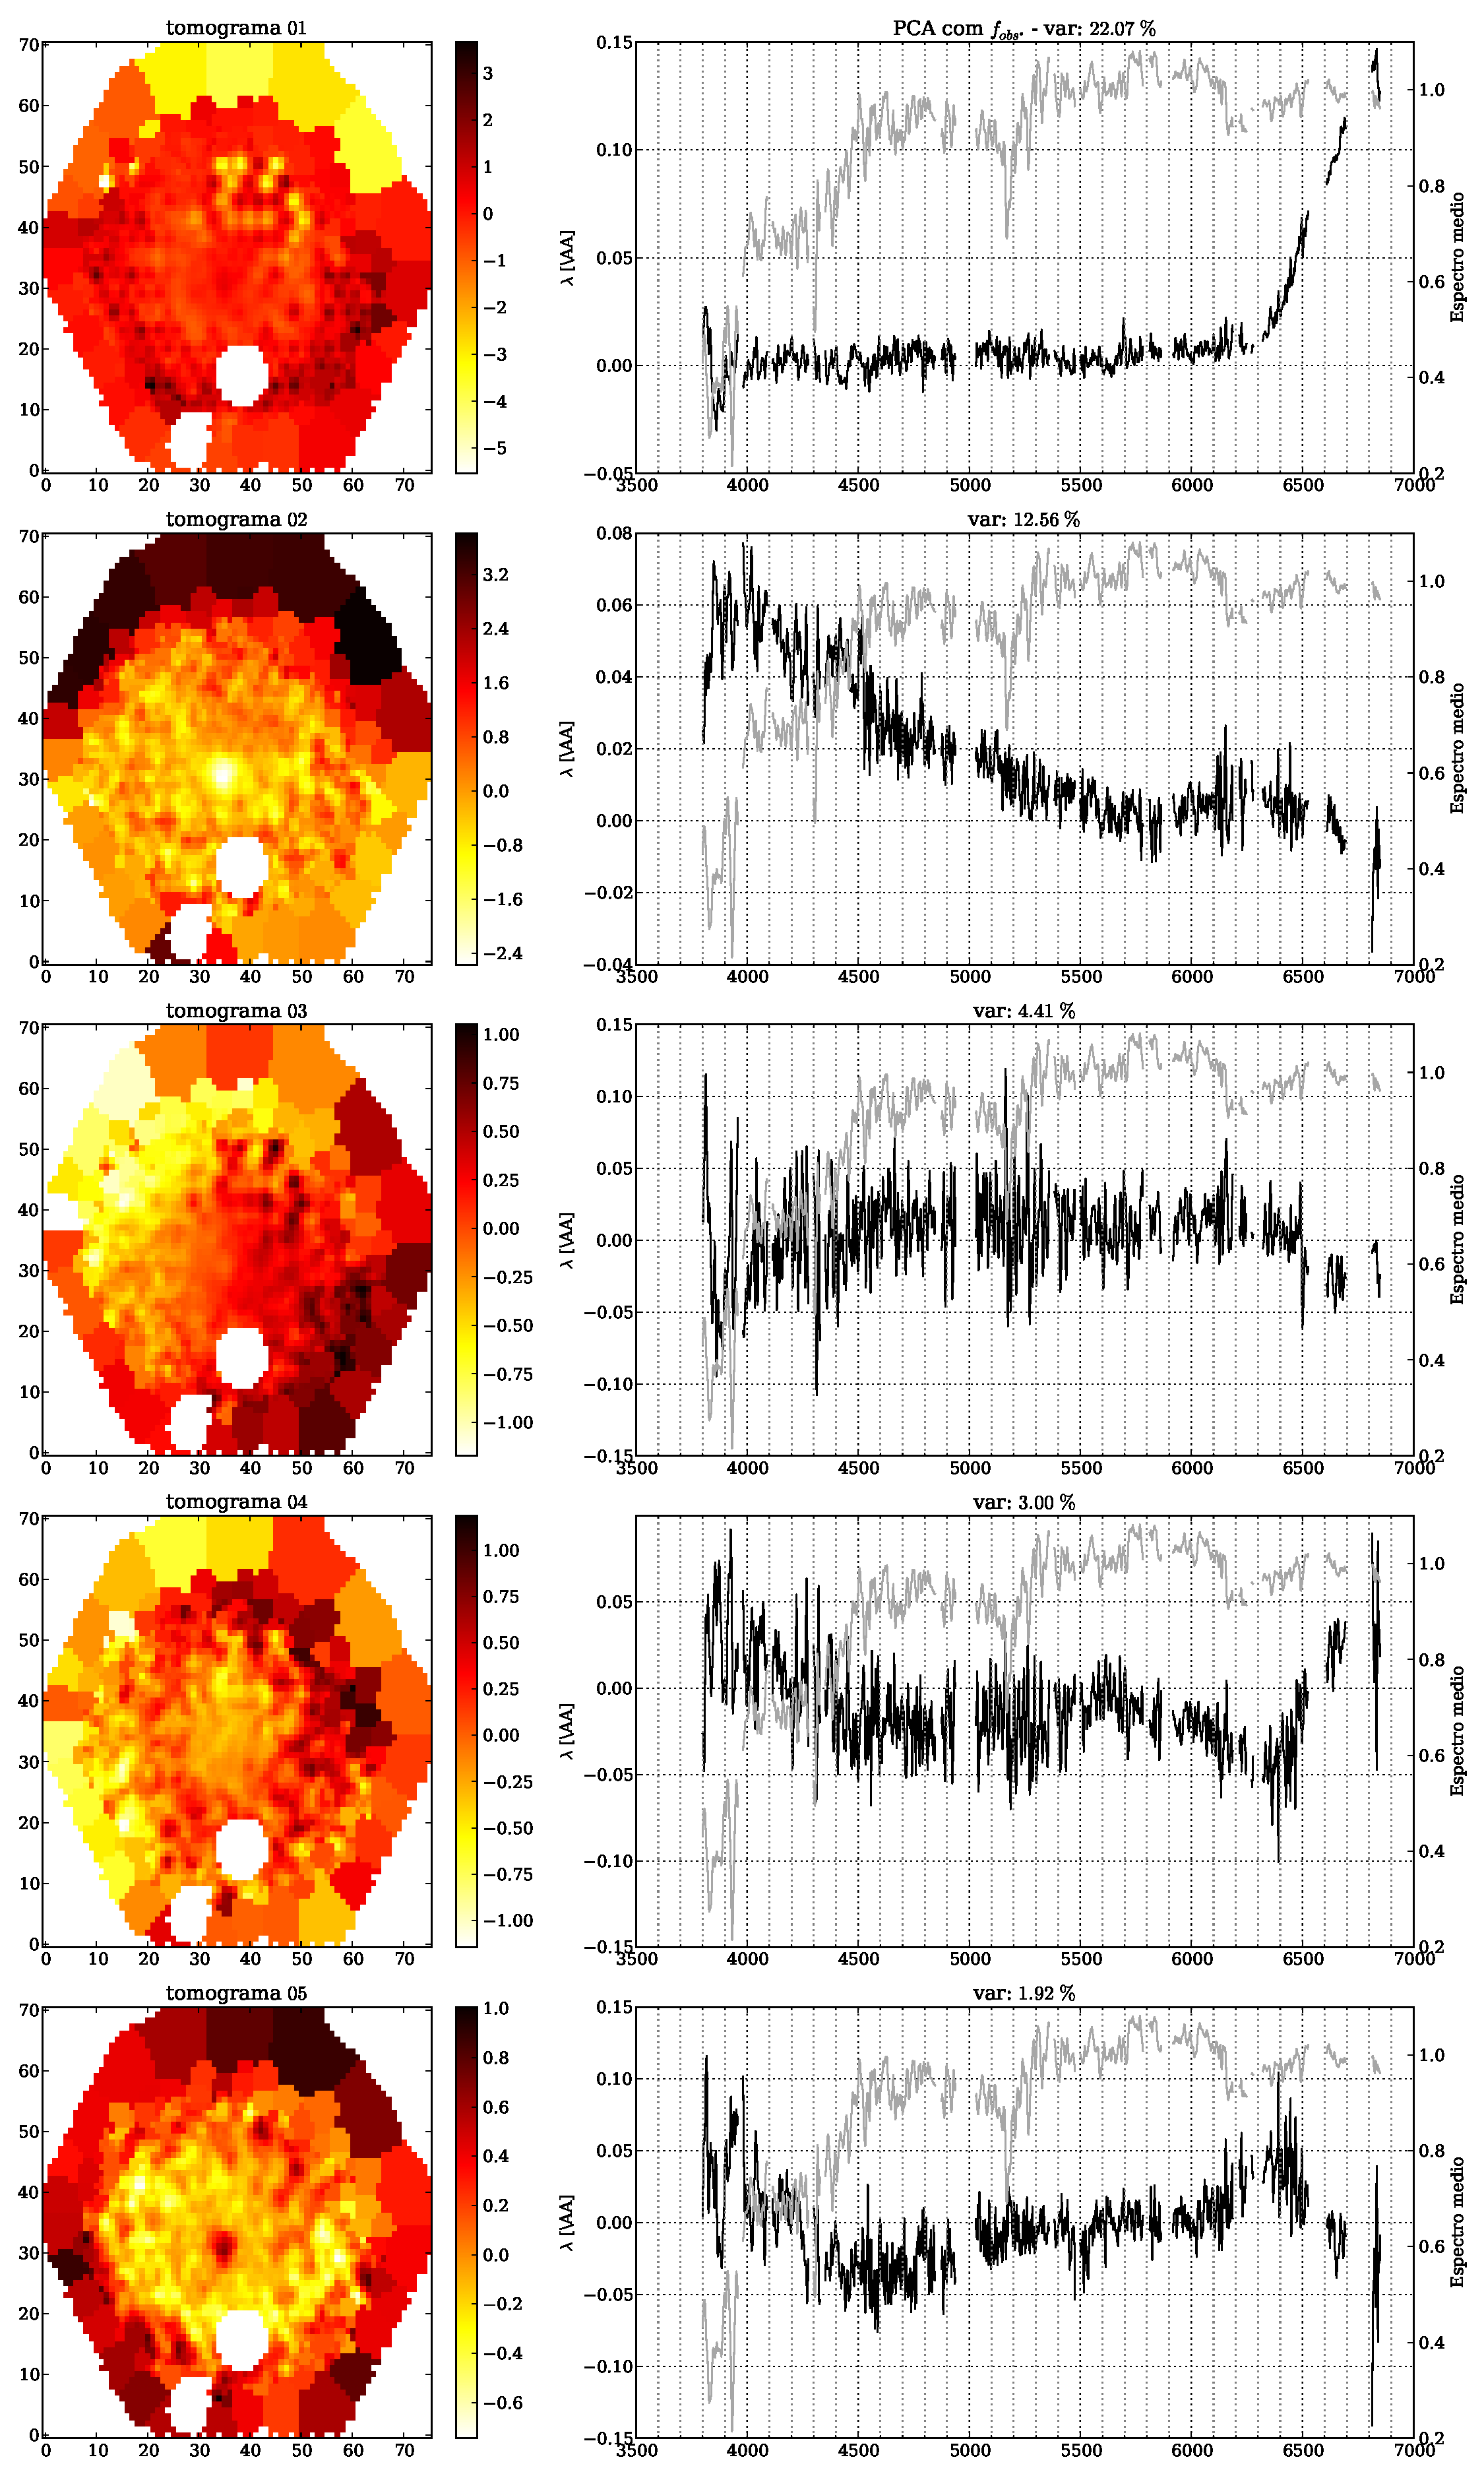
\includegraphics[width=0.85\textwidth]{figuras/K0119-tomo-obs-norm.pdf}
    \caption[Tomogramas de 1 a 5 para o cubo $F_{obs}$ norm. - NGC 1167.]
    {Igual a Figura \ref{fig:K0008tomofobsnorm} para a galáxia NGC 1167.}
    \label{fig:K0119tomofobsnorm}
\end{figure}

\begin{figure}
    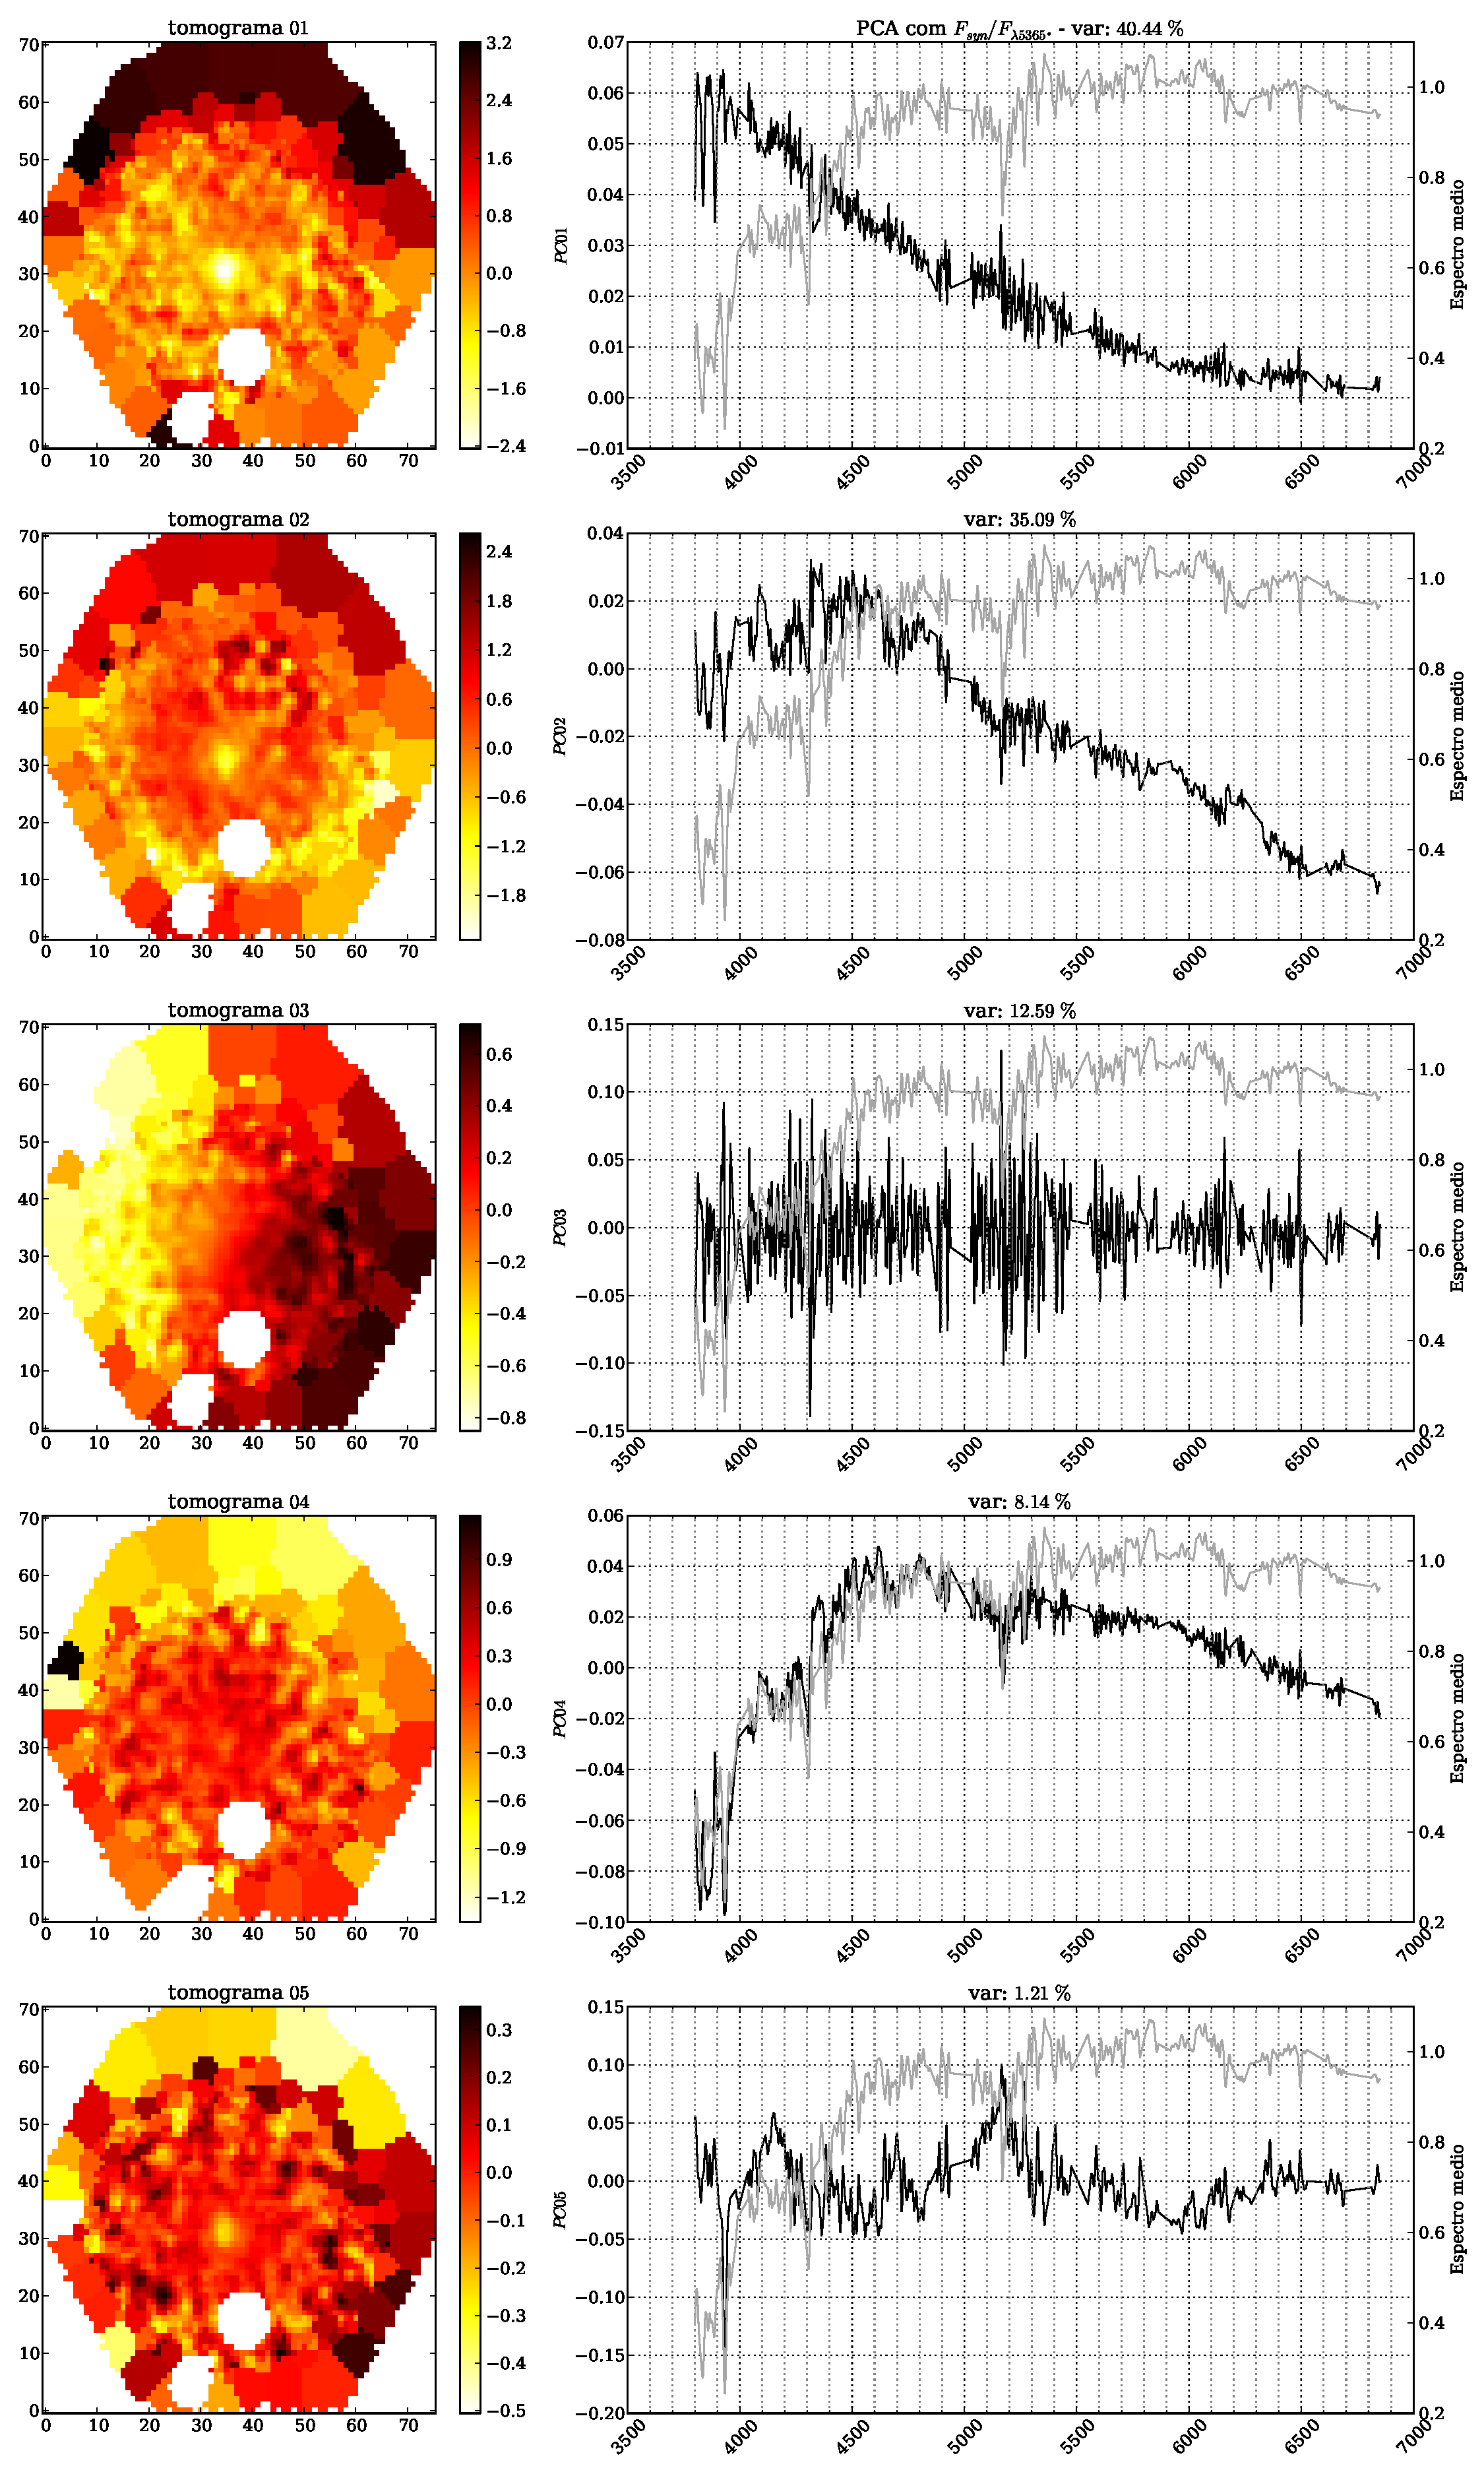
\includegraphics[width=0.85\textwidth]{figuras/K0119-tomo-syn-norm.pdf}
    \caption[Tomogramas de 1 a 5 para o cubo $F_{syn}$ norm. - NGC 1167.]
    {Igual a Figura \ref{fig:K0008tomofsynnorm} para a galáxia NGC 1167.}
    \label{fig:K0119tomofsynnorm}
\end{figure}

\begin{figure}
    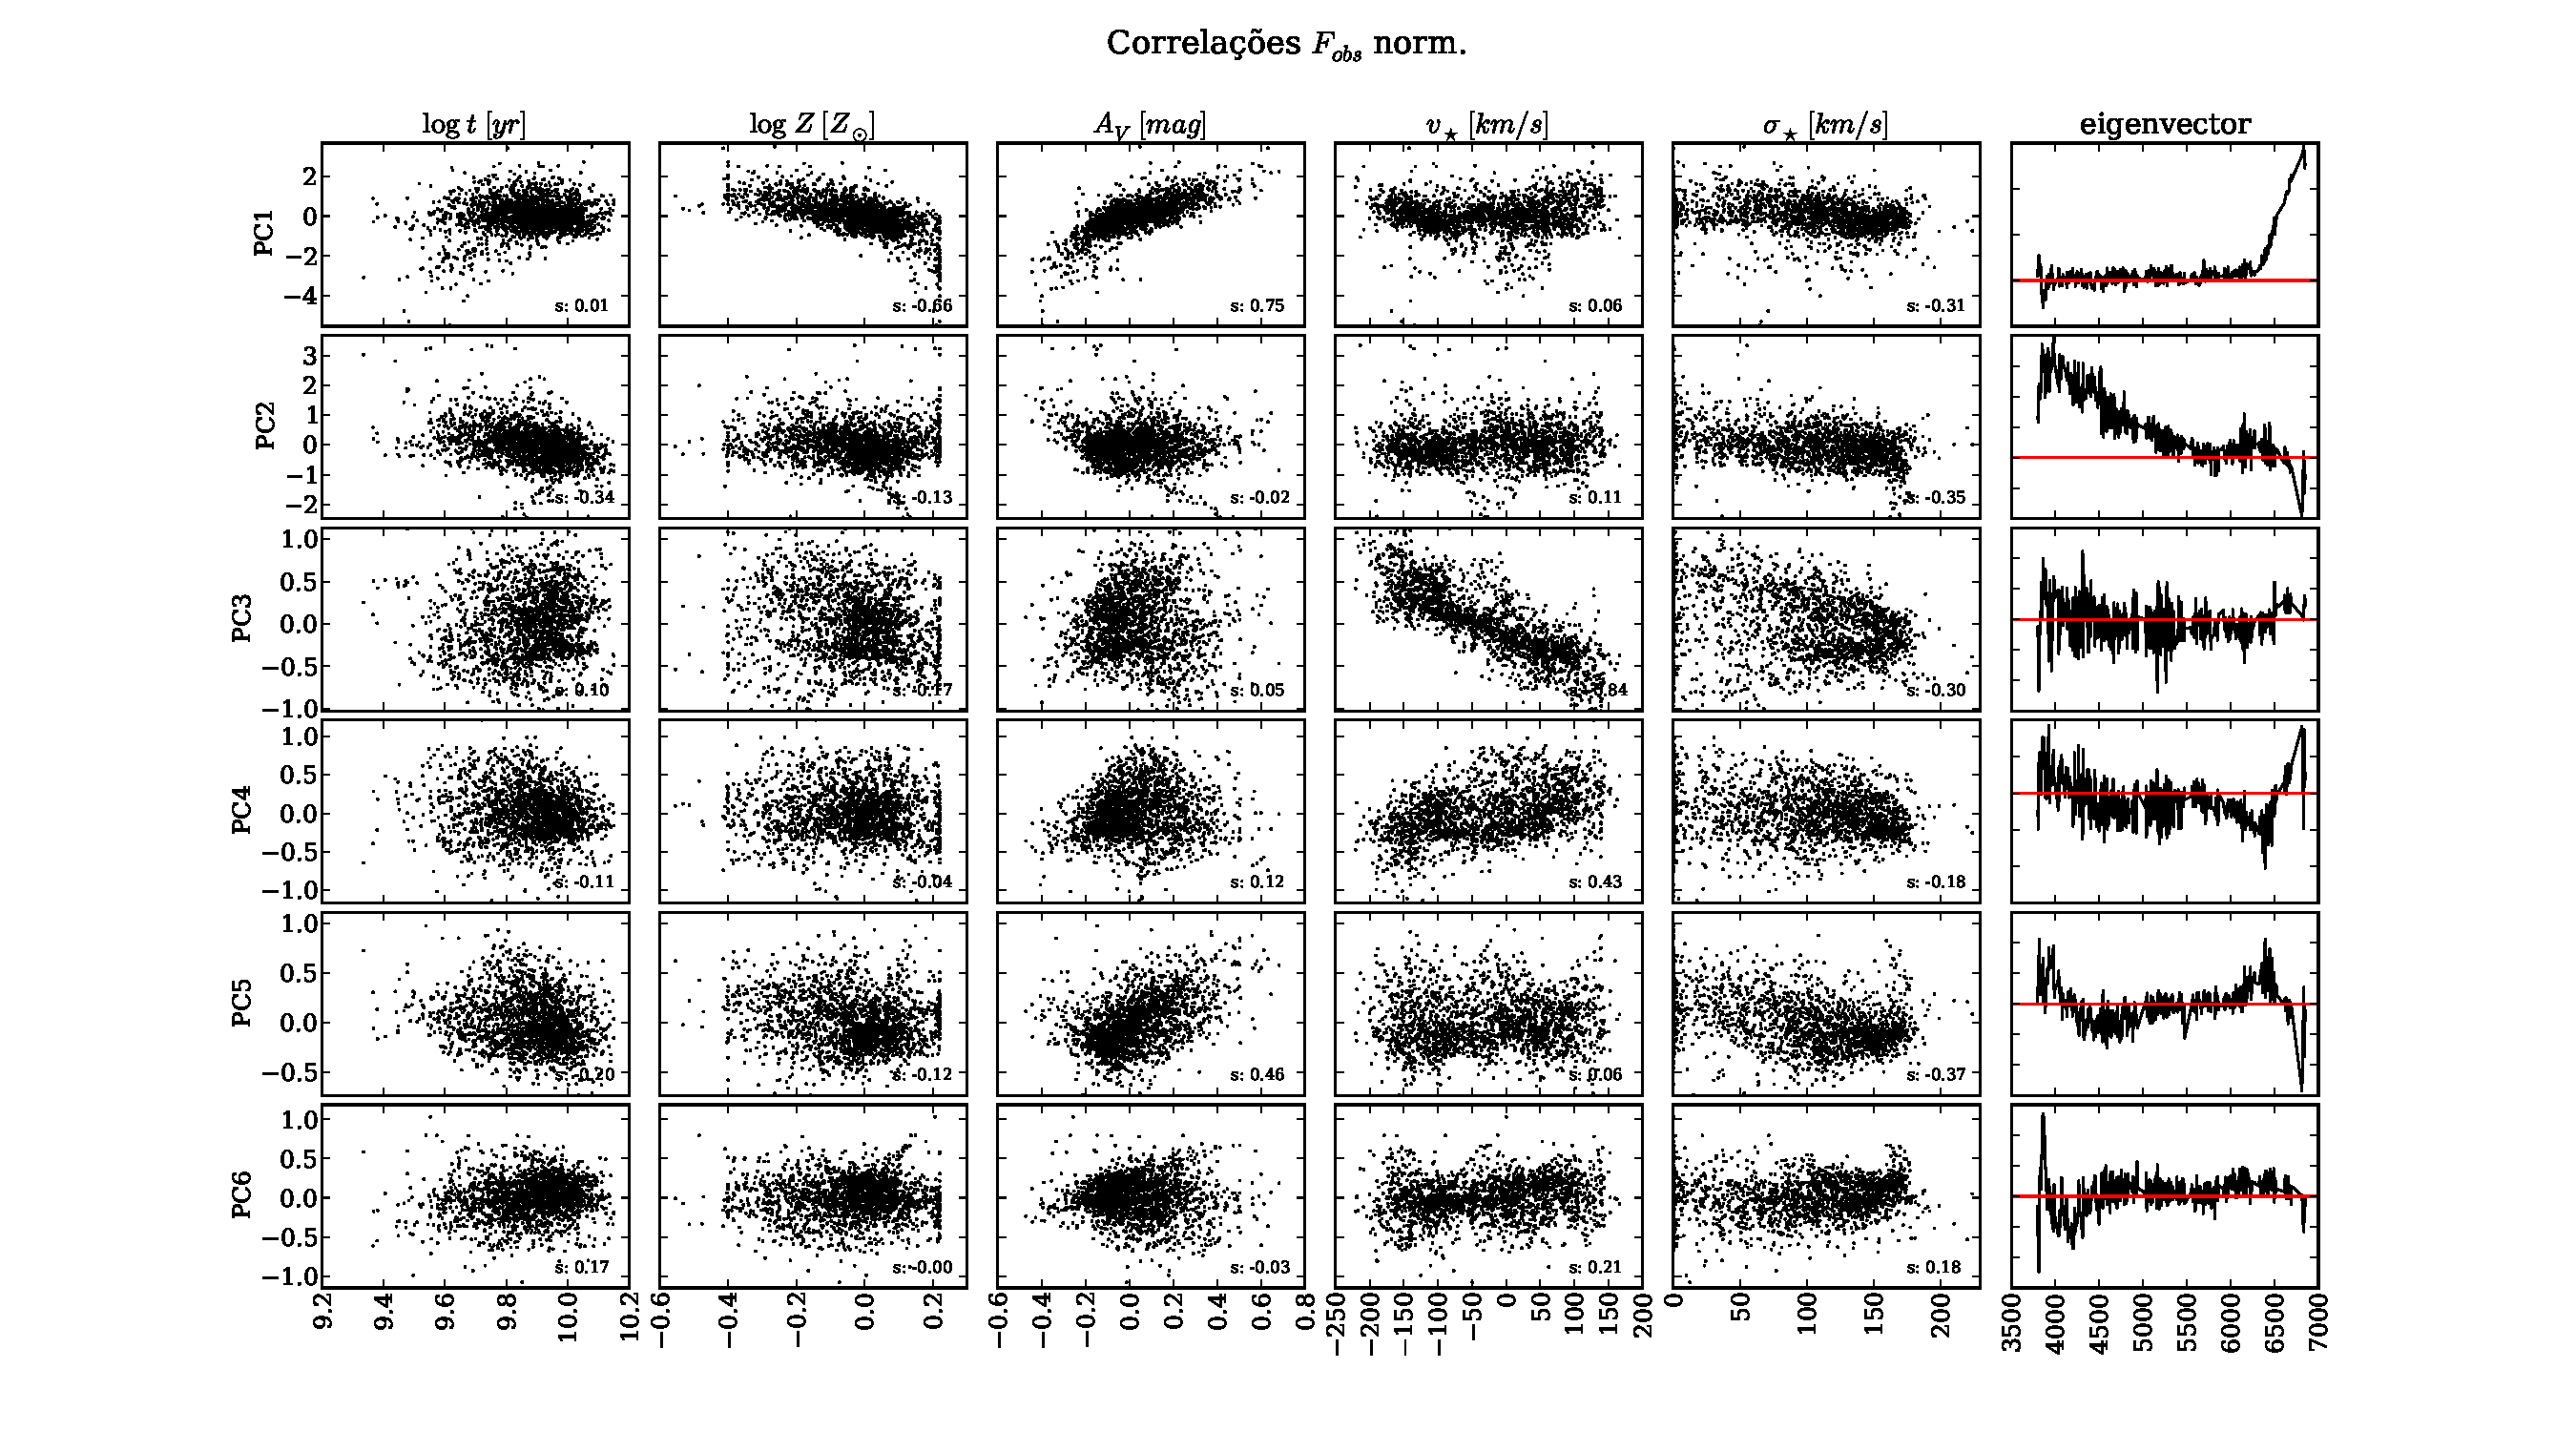
\includegraphics[width=1.3\textwidth, angle=-90]{figuras/K0119-correl-f_obs_norm-PCvsPhys.pdf}
	\caption[Correlações PCs vs. par\^ametros f\'isicos - $F_{obs}$ norm. - NGC 1167.]
	{Igual a Figura \ref{fig:K0008correfobsnorm} para a galáxia NGC 1167.}
    \label{fig:K0119correfobsnorm}
\end{figure}

\begin{figure}
    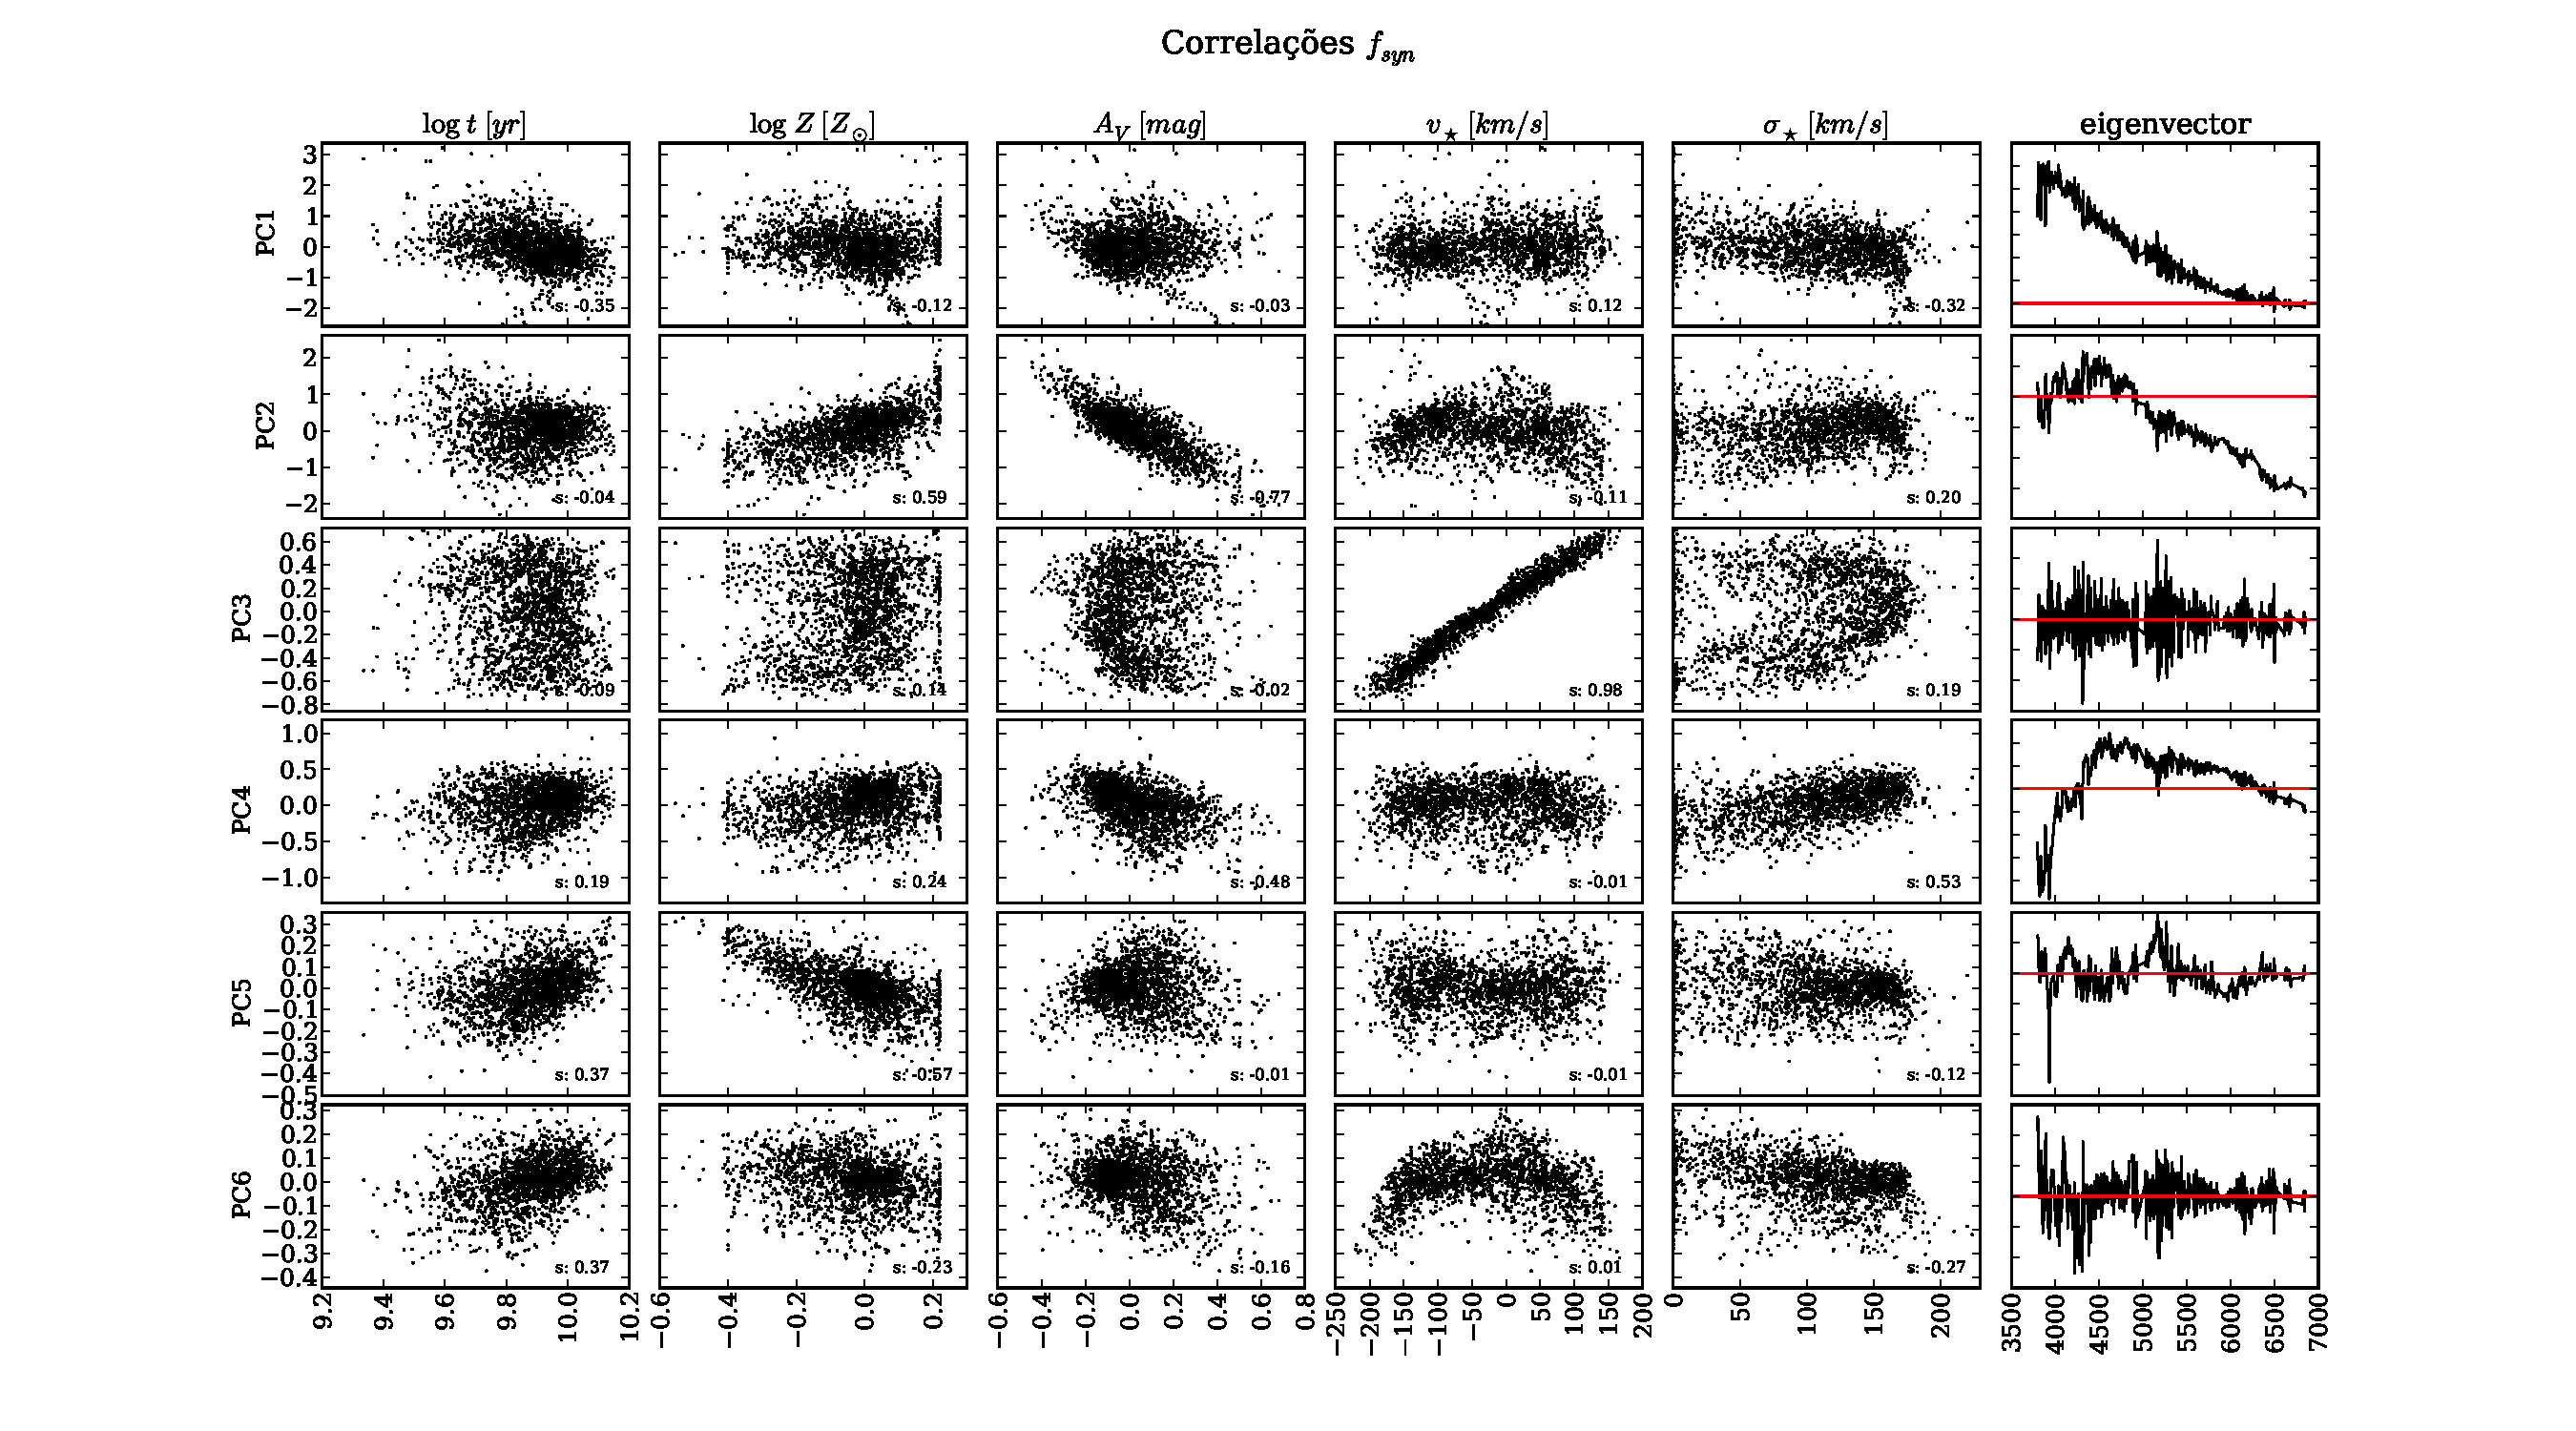
\includegraphics[width=1.3\textwidth, angle=-90]{figuras/K0119-correl-f_syn_norm-PCvsPhys.pdf}
	\caption[Correlações PCs vs. par\^ametros f\'isicos - $F_{syn}$ norm. - NGC 1167.]
	{Igual a Figura \ref{fig:K0008correfsynnorm} para a galáxia NGC 1167.}
    \label{fig:K0119correfsynnorm}
\end{figure}

\subsection{NGC 6515 - CALIFA 864}

\begin{figure}
    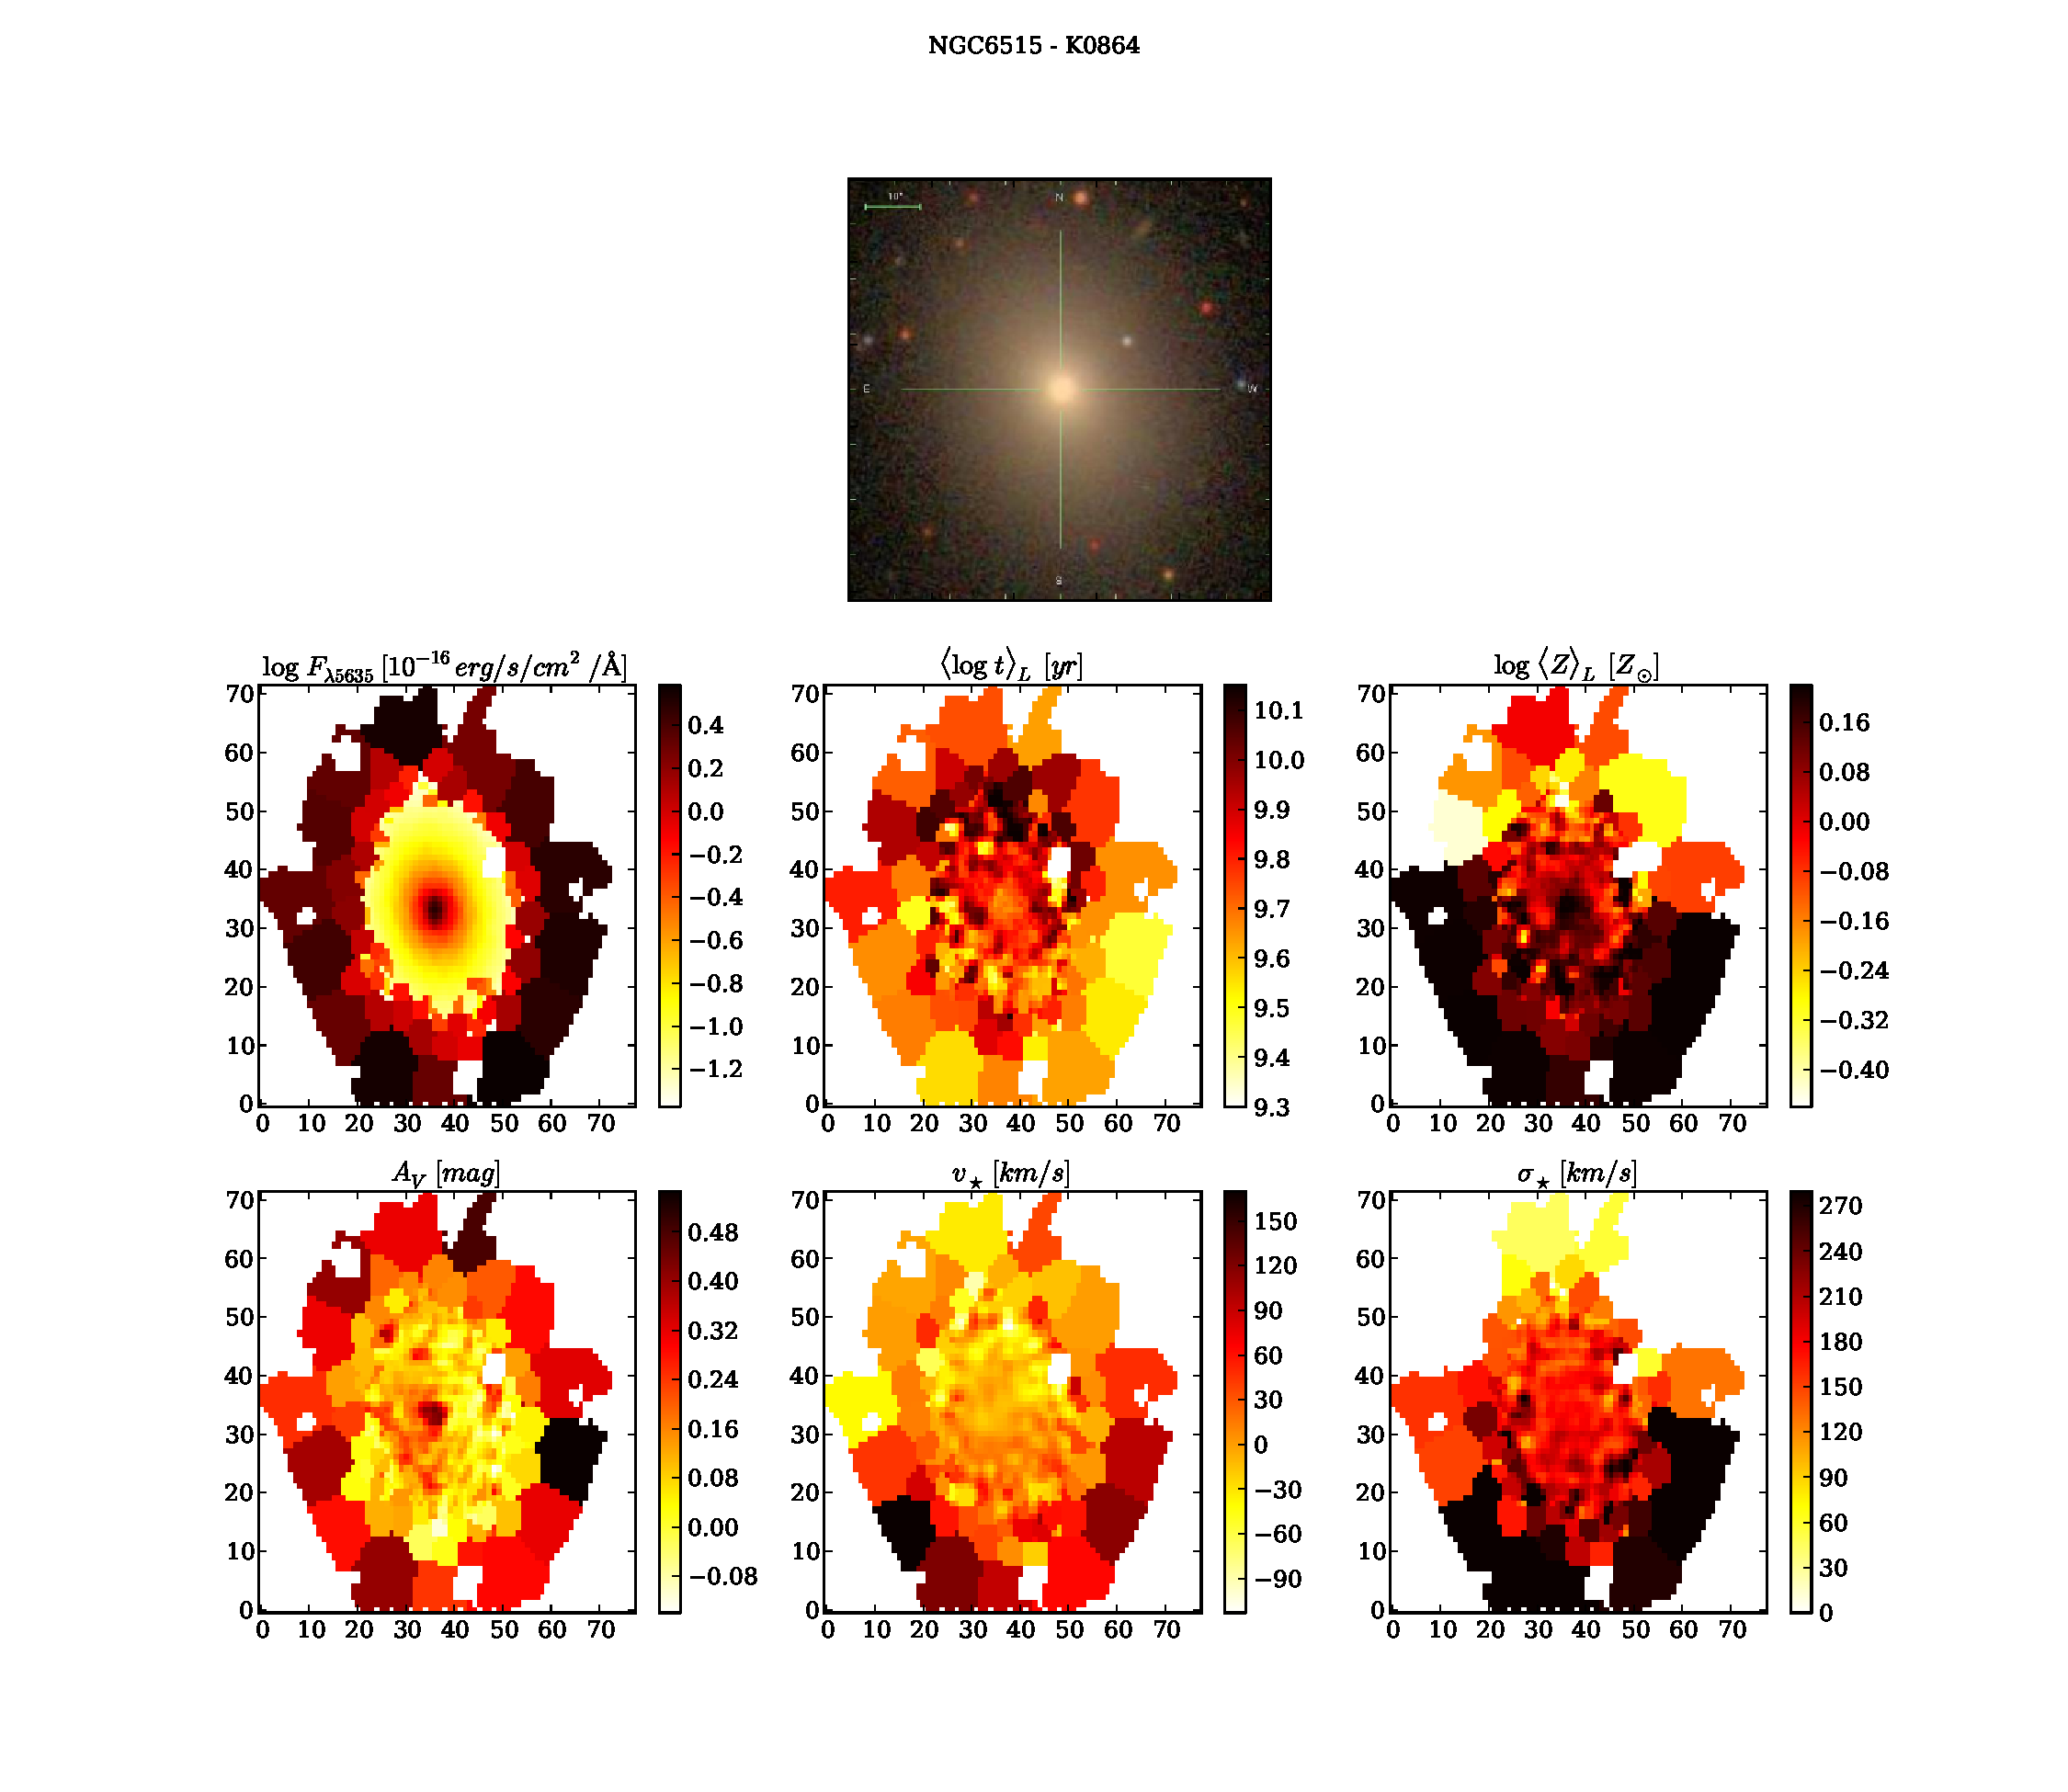
\includegraphics[width=1.\textwidth]{figuras/K0864-apresent.pdf}
    \caption[Propriedades f\'isicas da gal\'axia NGC 6515.]
    {Igual a Figura \ref{fig:K0008apresent} para a galáxia NGC 6515.}
    \label{fig:K0864apresent}
\end{figure}

\begin{figure}
    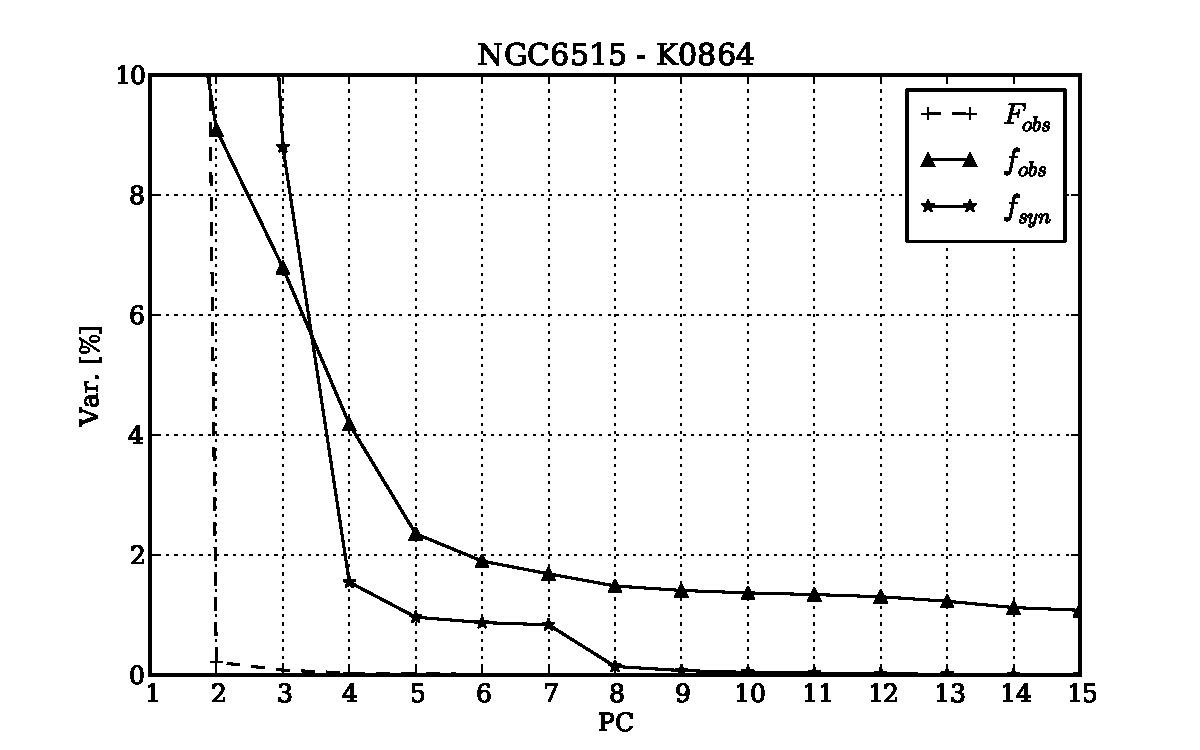
\includegraphics[height=0.33\textheight]{figuras/K0864-screetest.pdf}
    \caption[Scree test comparativo entre 3 PCAs - NGC 6515.]
	{Igual a Figura \ref{fig:K0008scree} para a galáxia NGC 6515.}
    \label{fig:K0864scree}
\end{figure}

\begin{figure}
    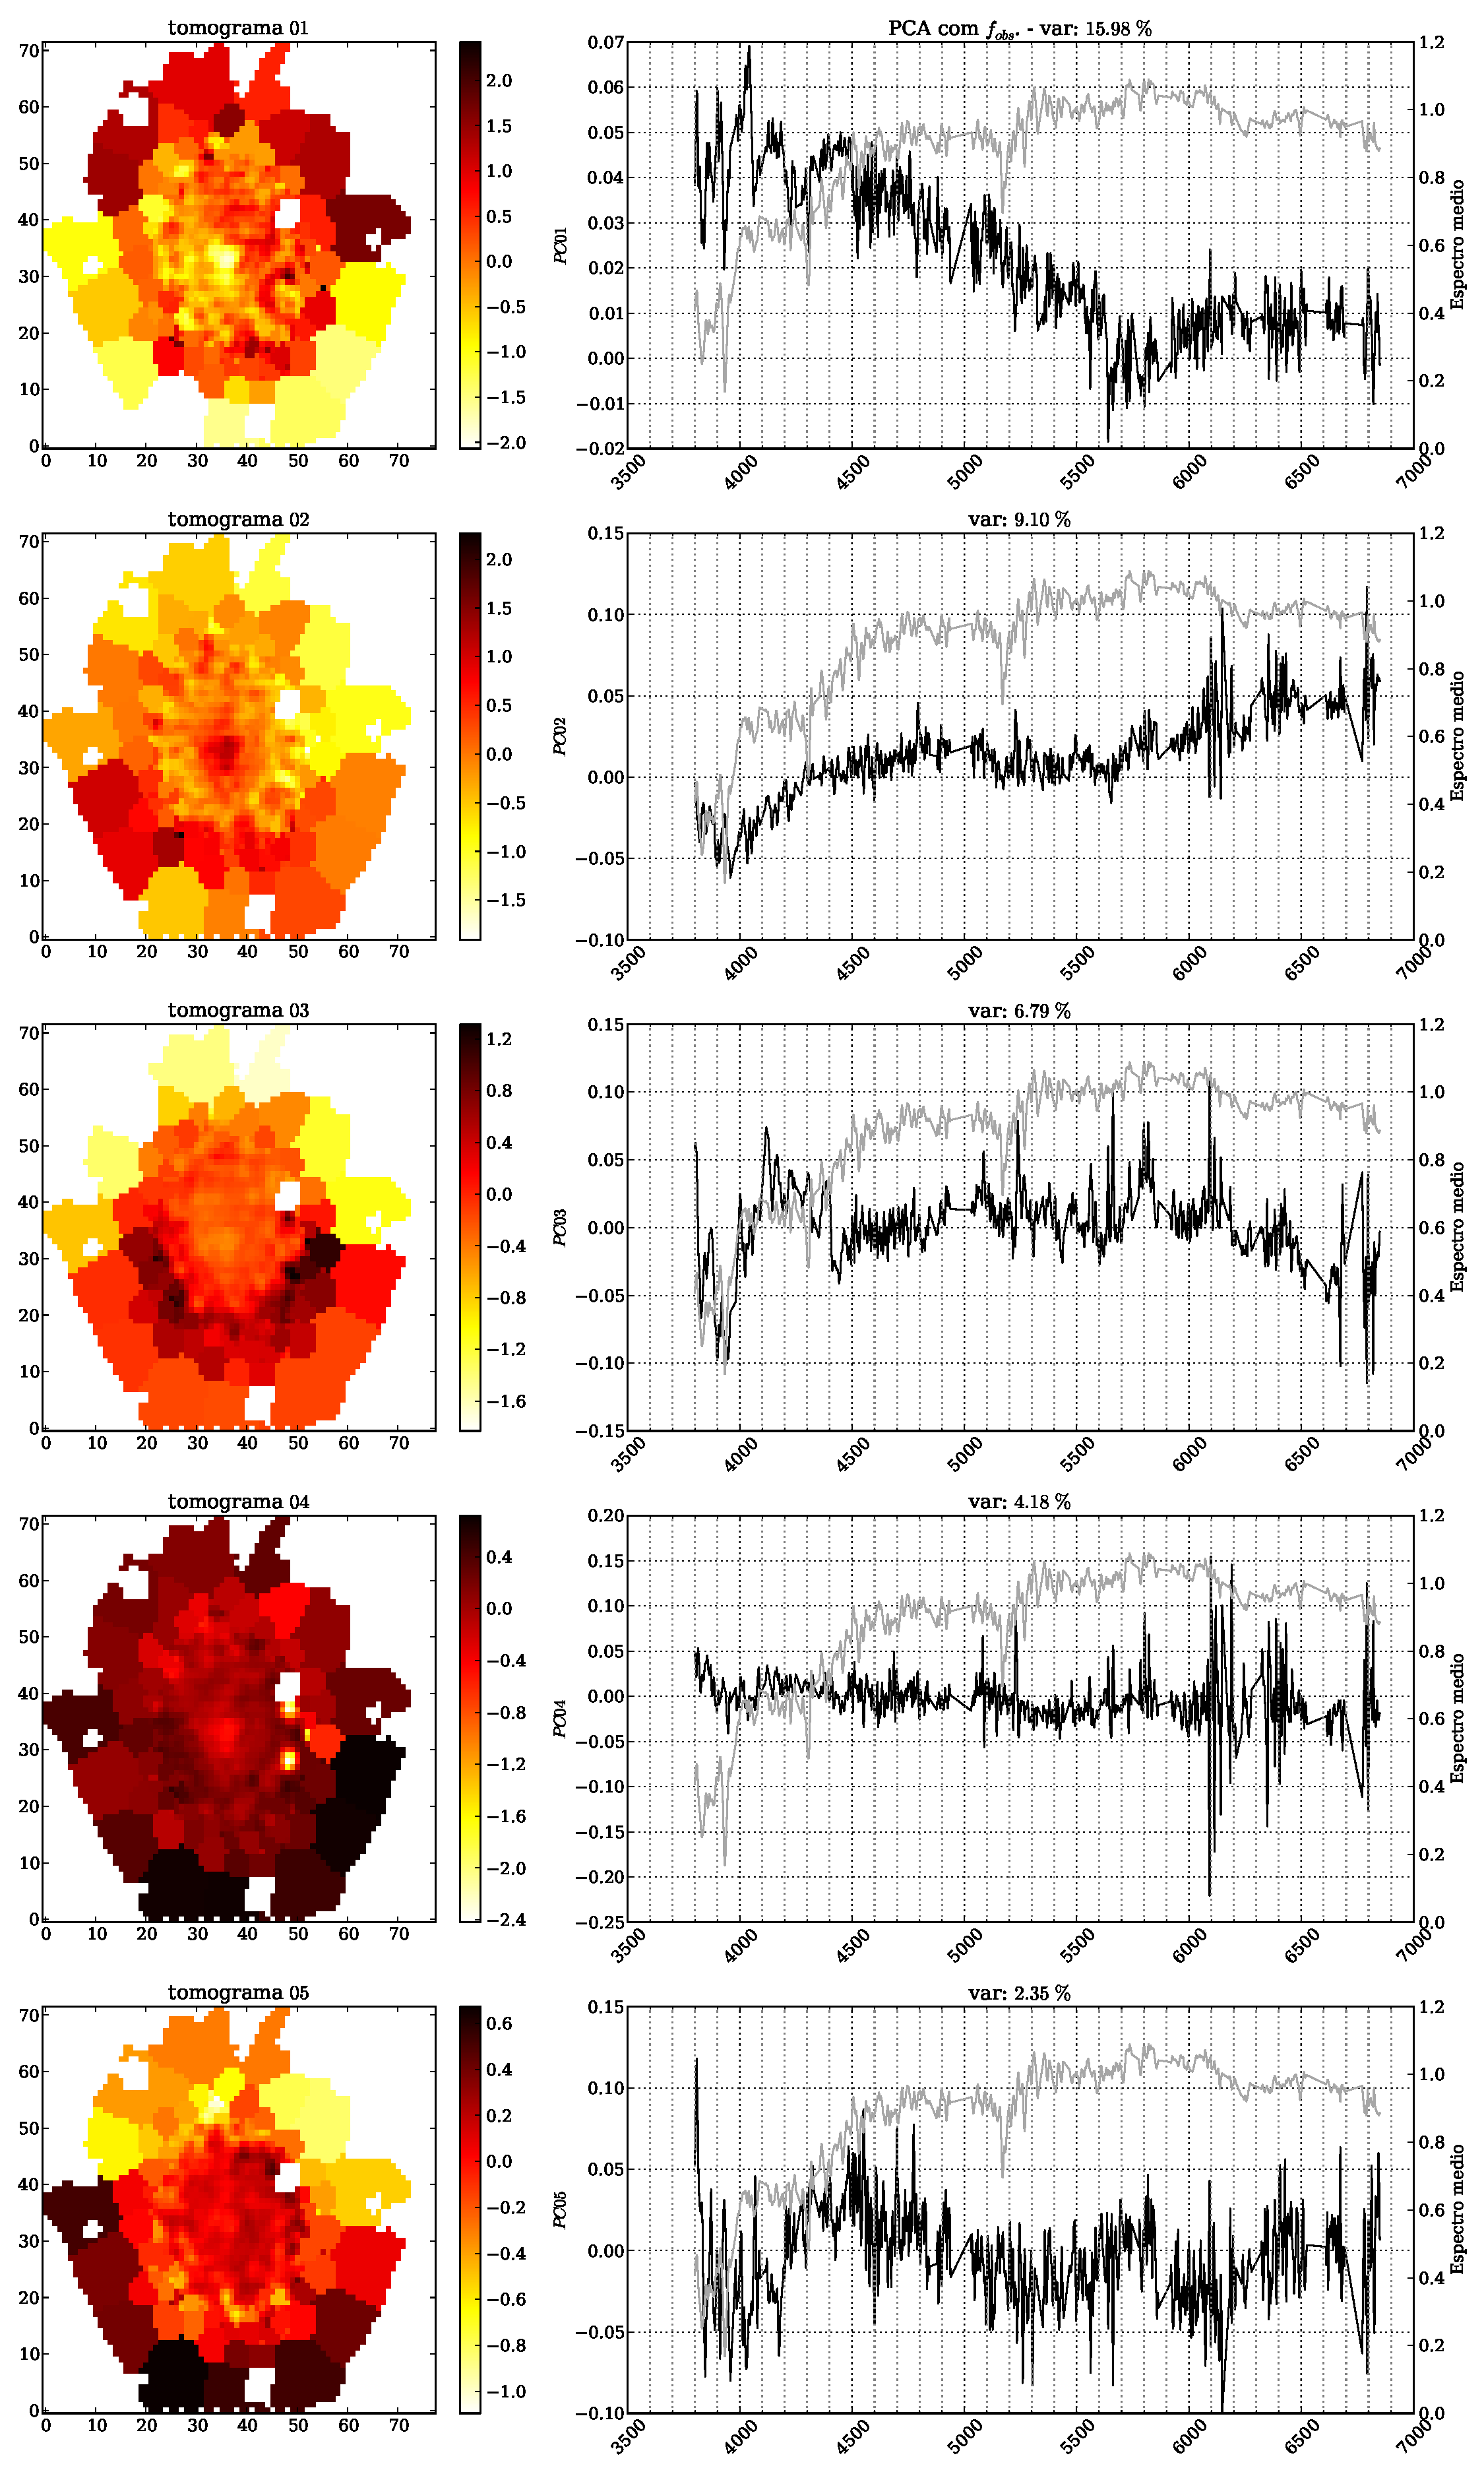
\includegraphics[width=0.85\textwidth]{figuras/K0864-tomo-obs-norm.pdf}
    \caption[Tomogramas de 1 a 5 para o cubo $F_{obs}$ norm. - NGC 6515.]
    {Igual a Figura \ref{fig:K0008tomofobsnorm} para a galáxia NGC 6515.}
    \label{fig:K0864tomofobsnorm}
\end{figure}

\begin{figure}
    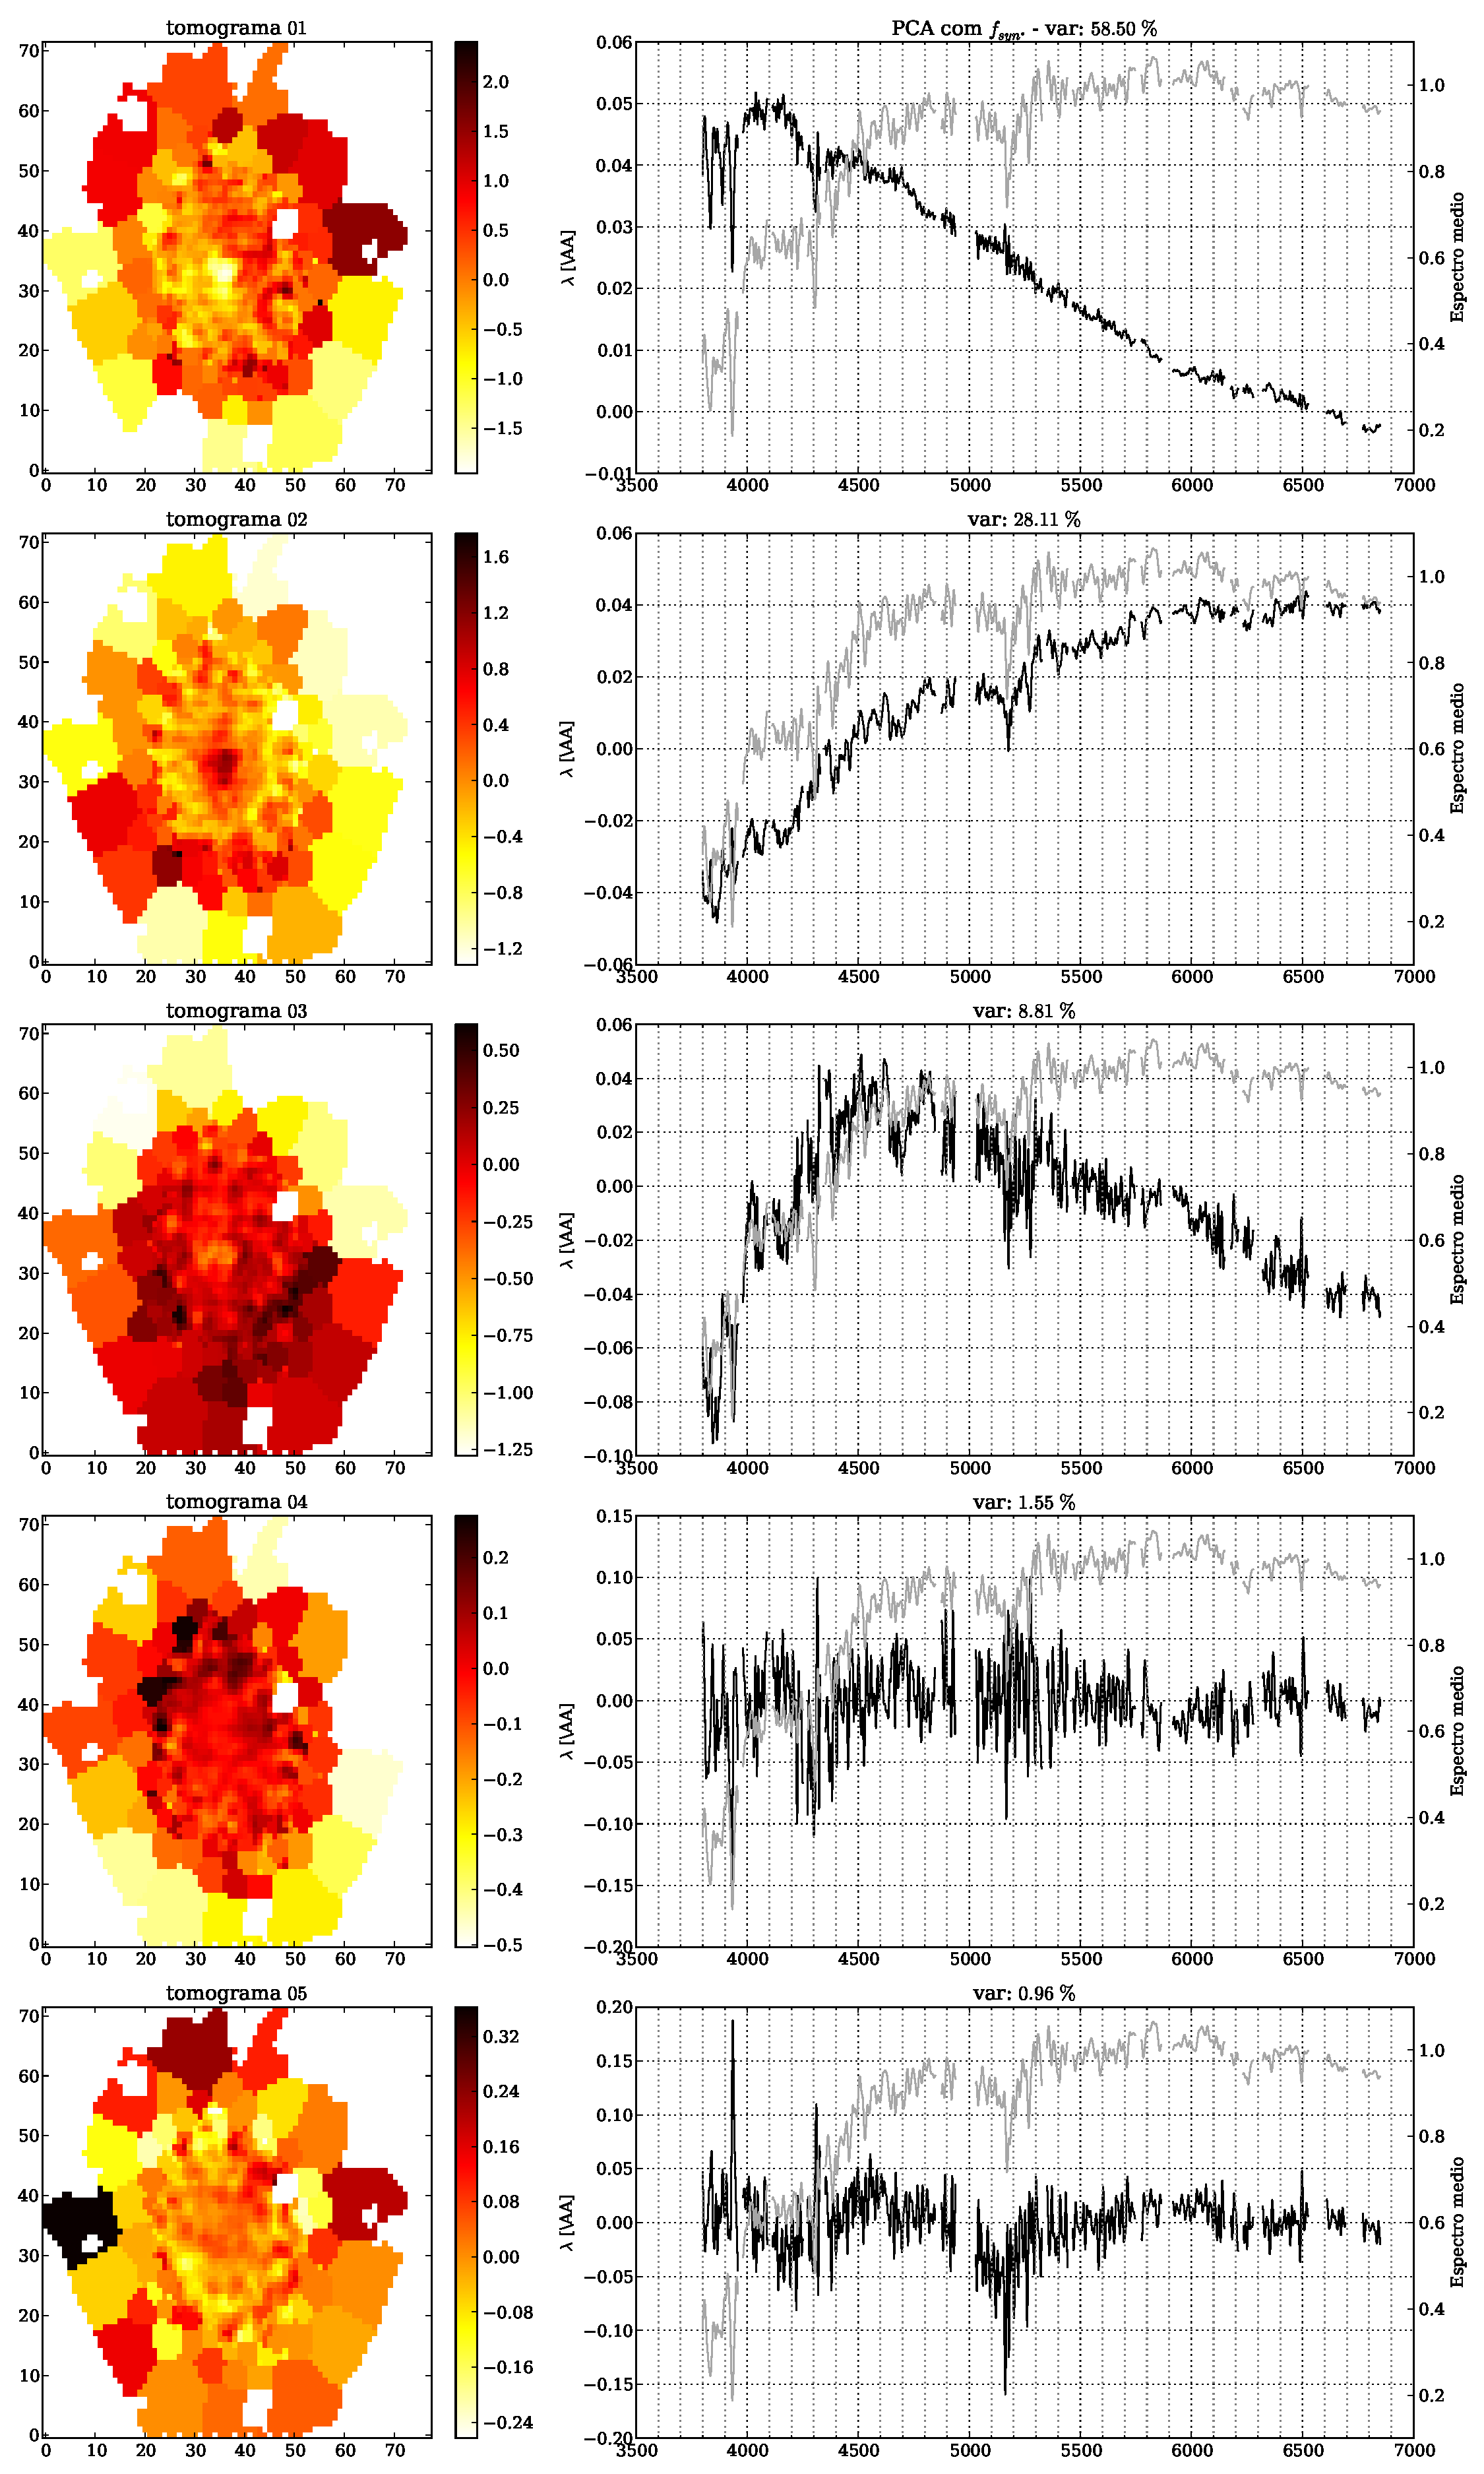
\includegraphics[width=0.85\textwidth]{figuras/K0864-tomo-syn-norm.pdf}
    \caption[Tomogramas de 1 a 5 para o cubo $F_{syn}$ norm. - NGC 6515.]
    {Igual a Figura \ref{fig:K0008tomofsynnorm} para a galáxia NGC 6515.}
    \label{fig:K0864tomofsynnorm}
\end{figure}

\begin{figure}
    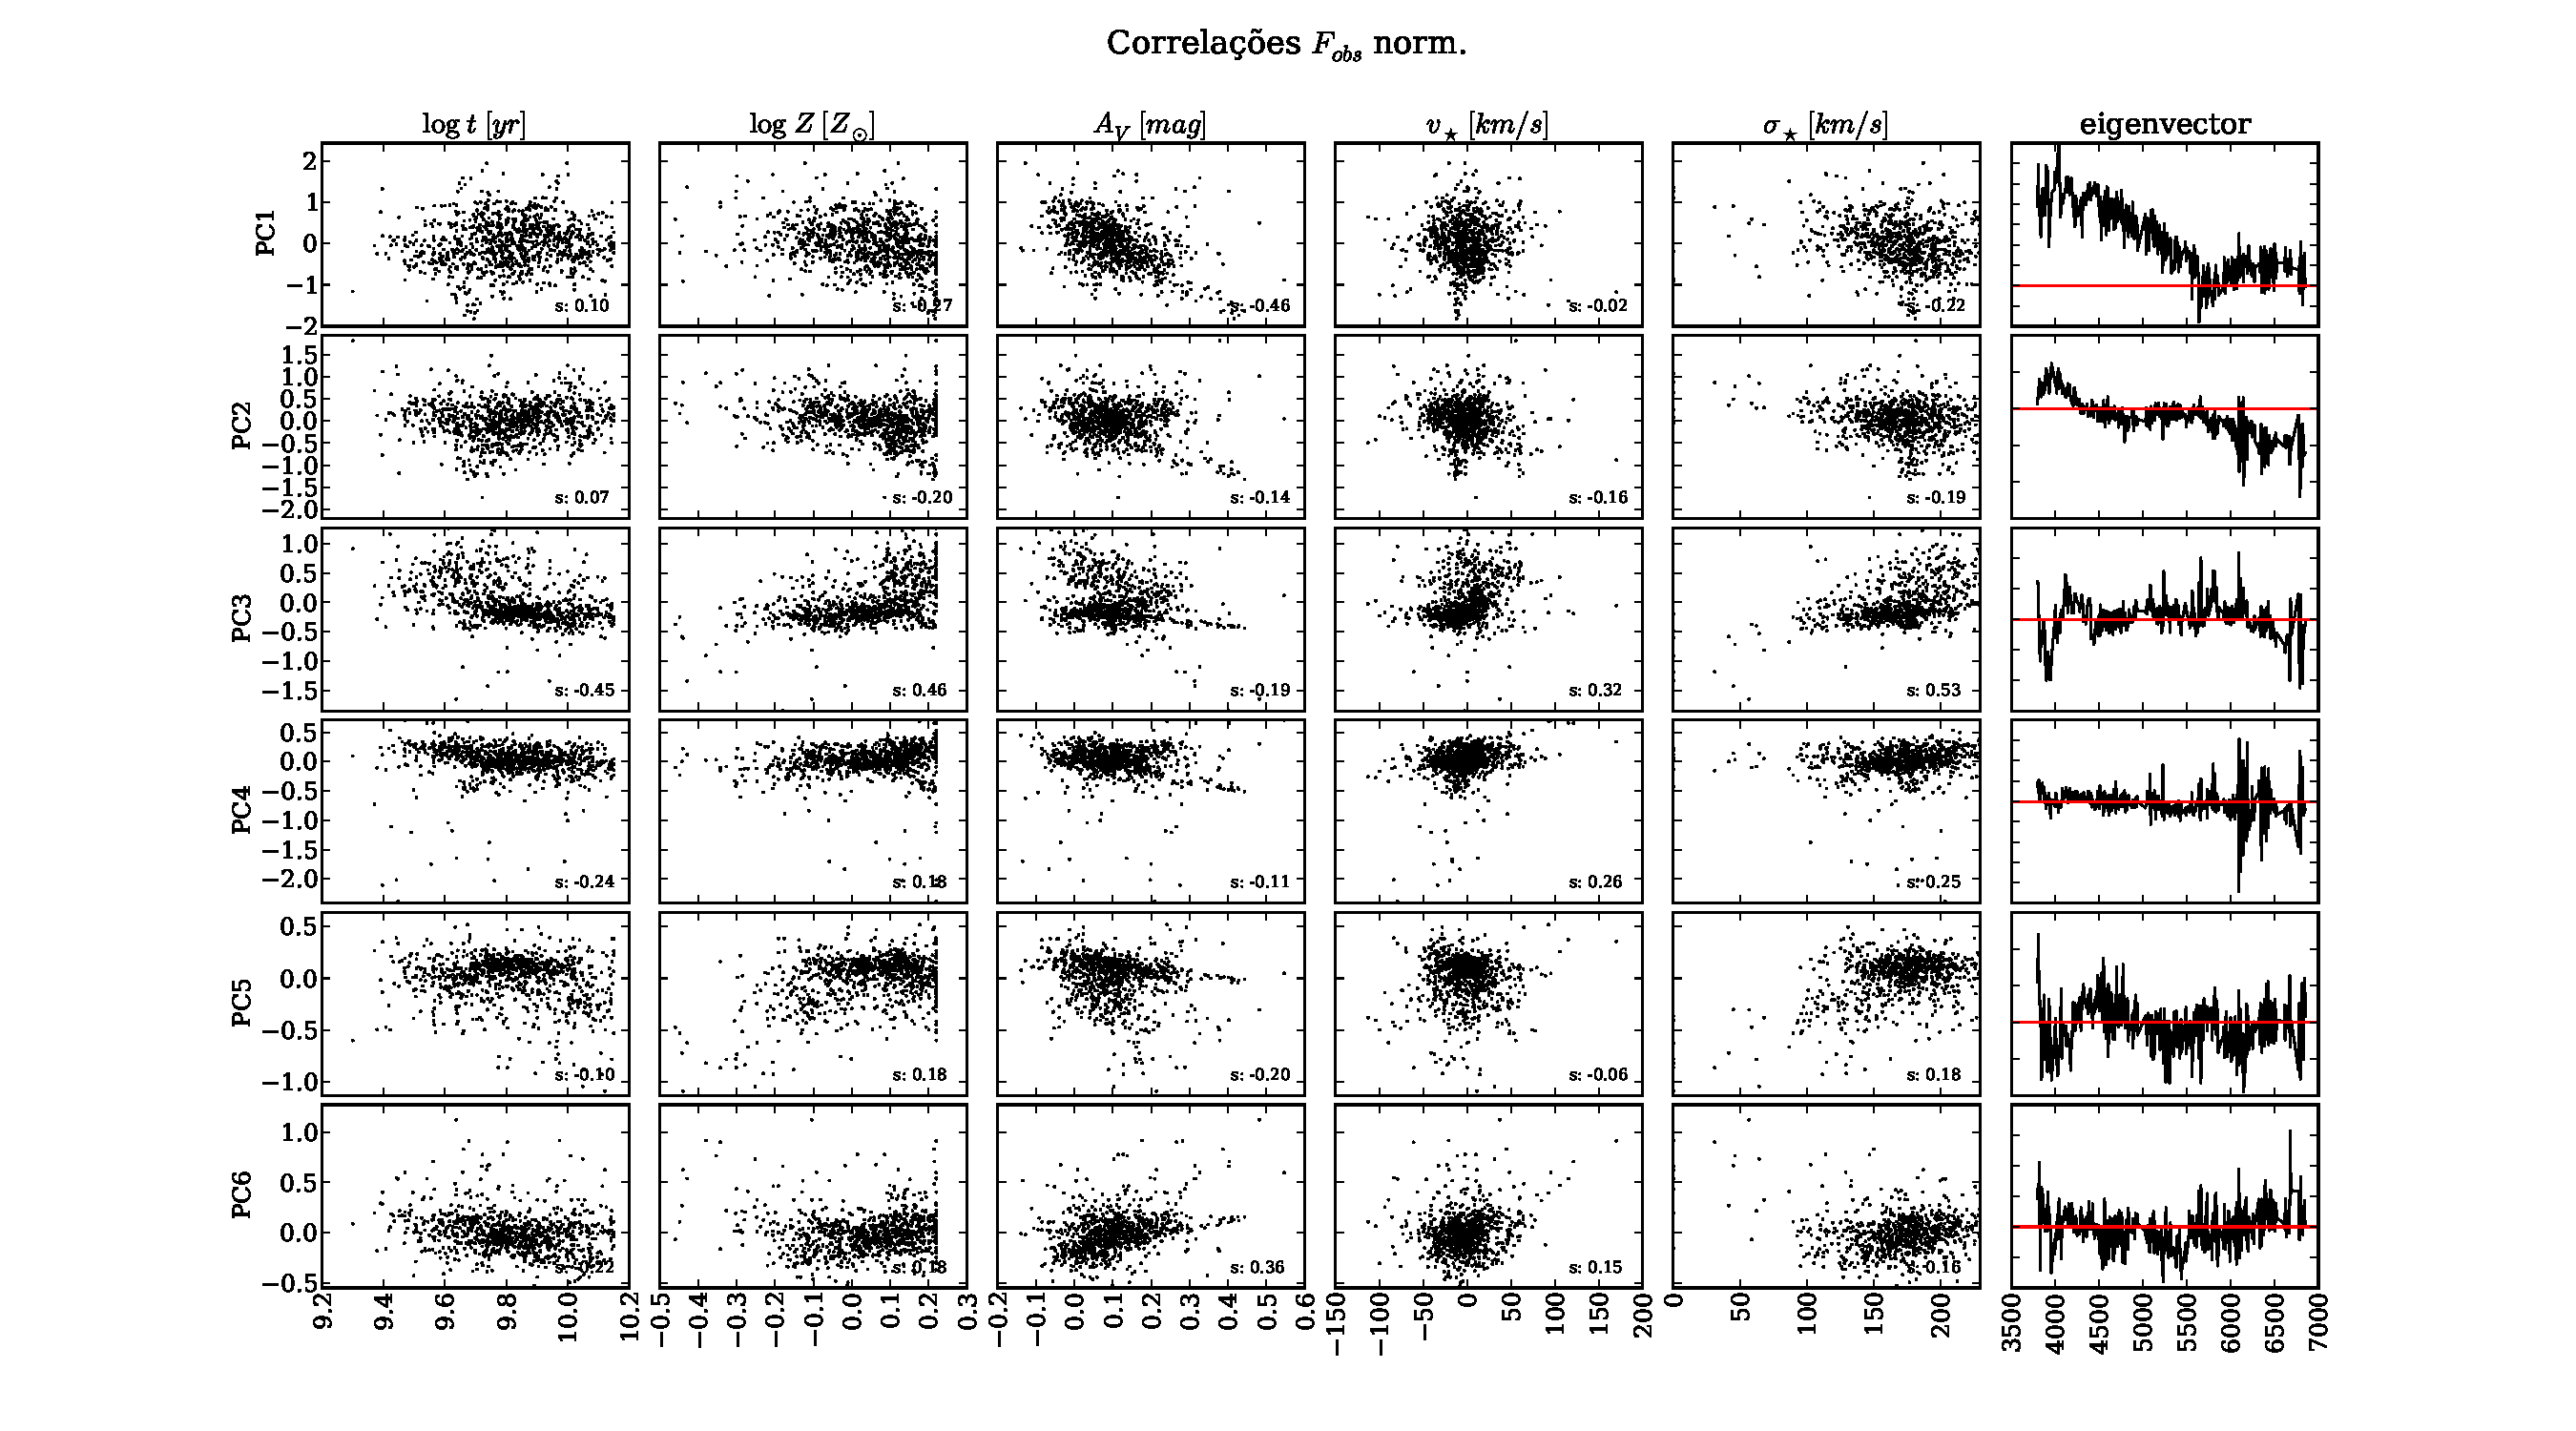
\includegraphics[width=1.3\textwidth, angle=-90]{figuras/K0864-correl-f_obs_norm-PCvsPhys.pdf}
	\caption[Correlações PCs vs. par\^ametros f\'isicos - $F_{obs}$ norm. - NGC 6515.]
	{Igual a Figura \ref{fig:K0008correfobsnorm} para a galáxia NGC 6515.}
    \label{fig:K0864correfobsnorm}
\end{figure}

\begin{figure}
    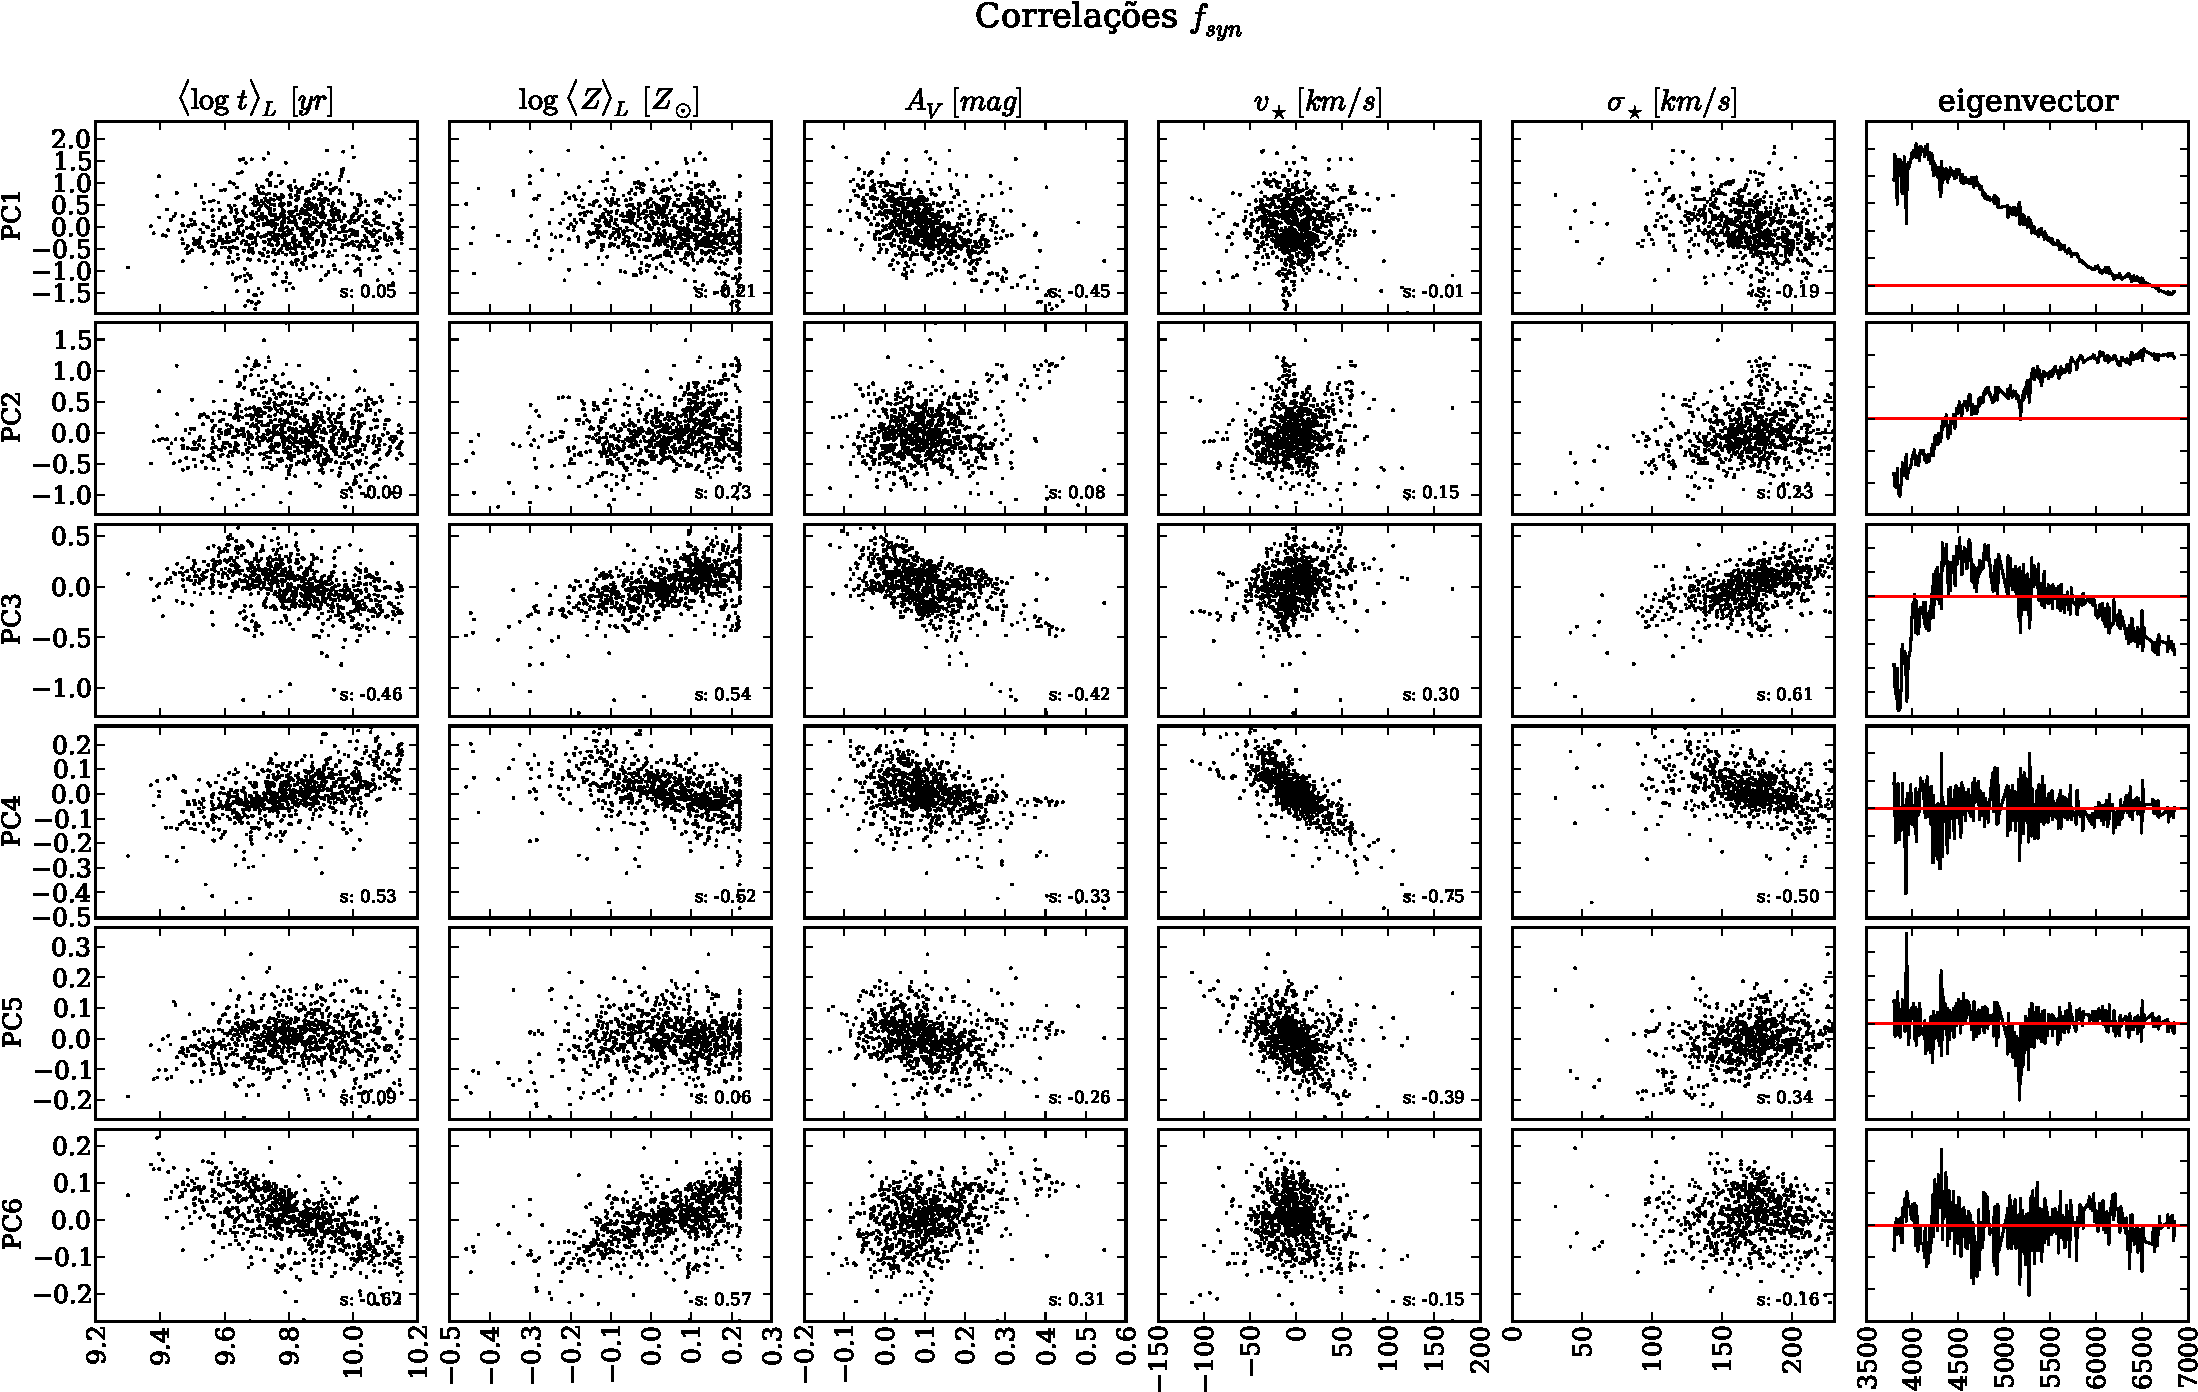
\includegraphics[width=1.3\textwidth, angle=-90]{figuras/K0864-correl-f_syn_norm-PCvsPhys.pdf}
	\caption[Correlações PCs vs. par\^ametros f\'isicos - $F_{syn}$ norm. - NGC 6515.]
	{Igual a Figura \ref{fig:K0008correfsynnorm} para a galáxia NGC 6515.}
    \label{fig:K0864correfsynnorm}
\end{figure}

\section{{\em Mergers}}
\ref{sec:result:mergers}

\subsection{NGC 2623 - CALIFA 213}

\begin{figure}
    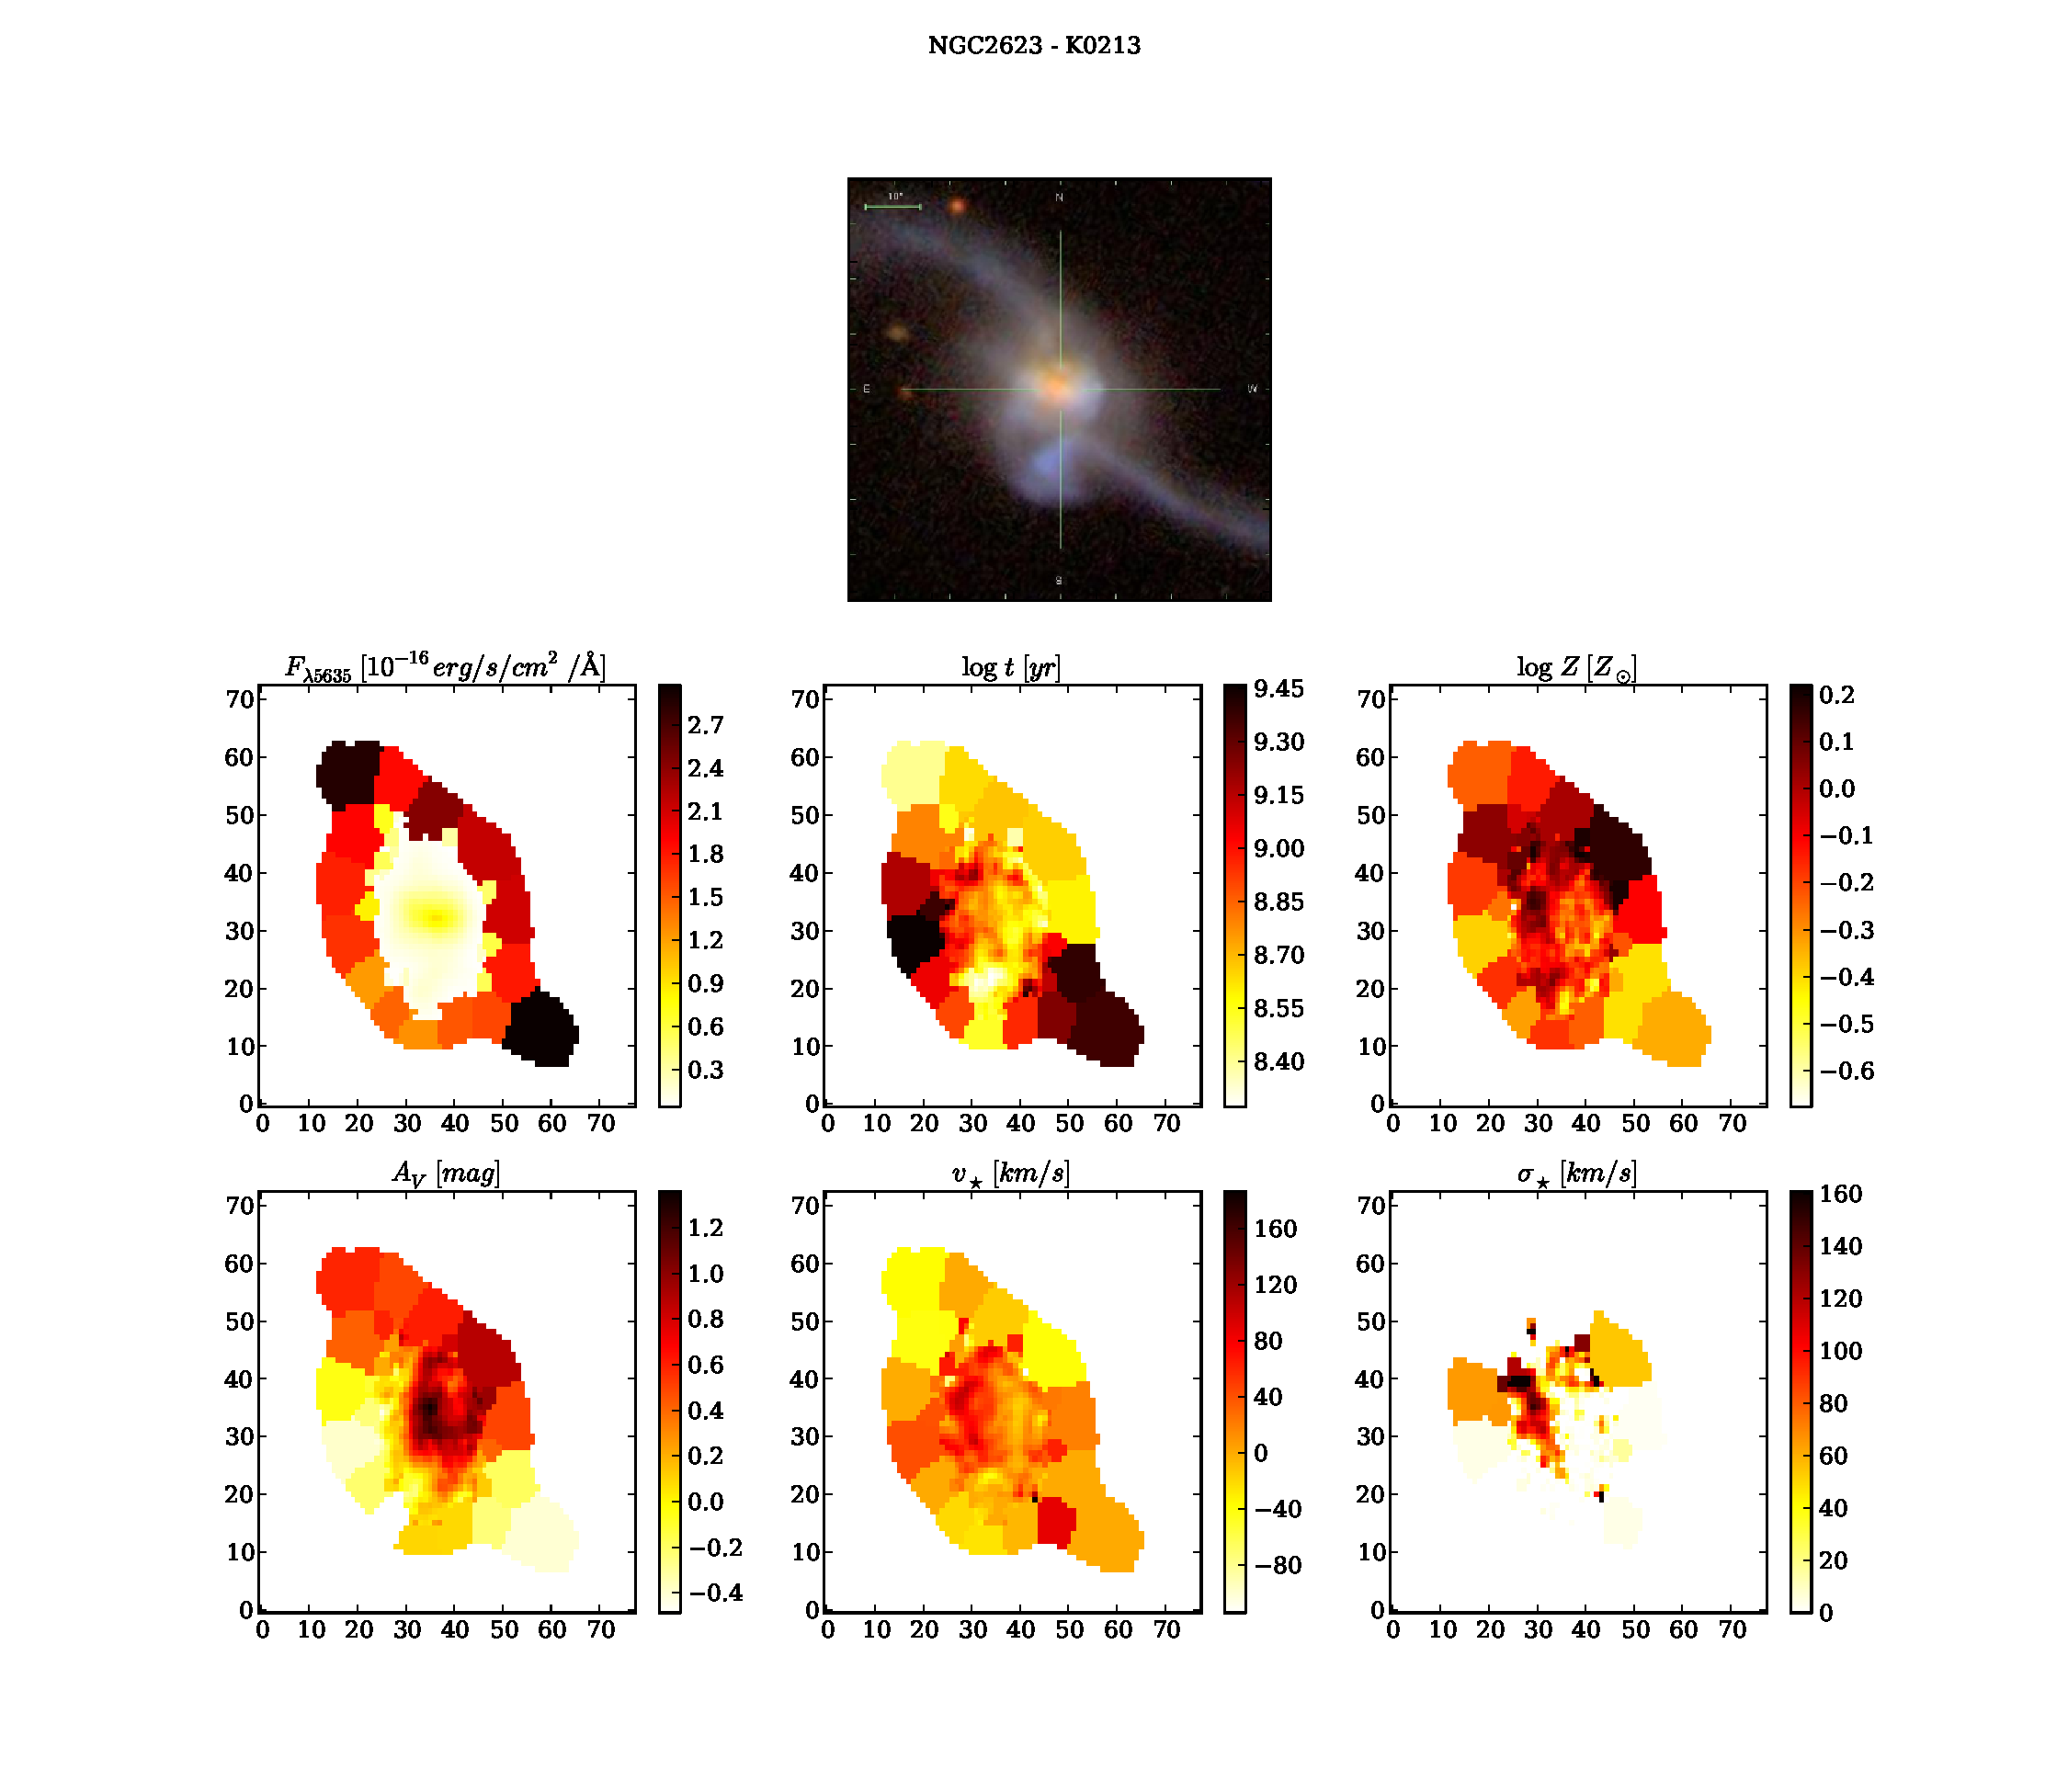
\includegraphics[width=1.\textwidth]{figuras/K0213-apresent.pdf}
    \caption[Propriedades f\'isicas da gal\'axia NGC 2623.]
    {Igual a Figura \ref{fig:K0008apresent} para a galáxia NGC 2623.}
    \label{fig:K0213apresent}
\end{figure}

\begin{figure}
    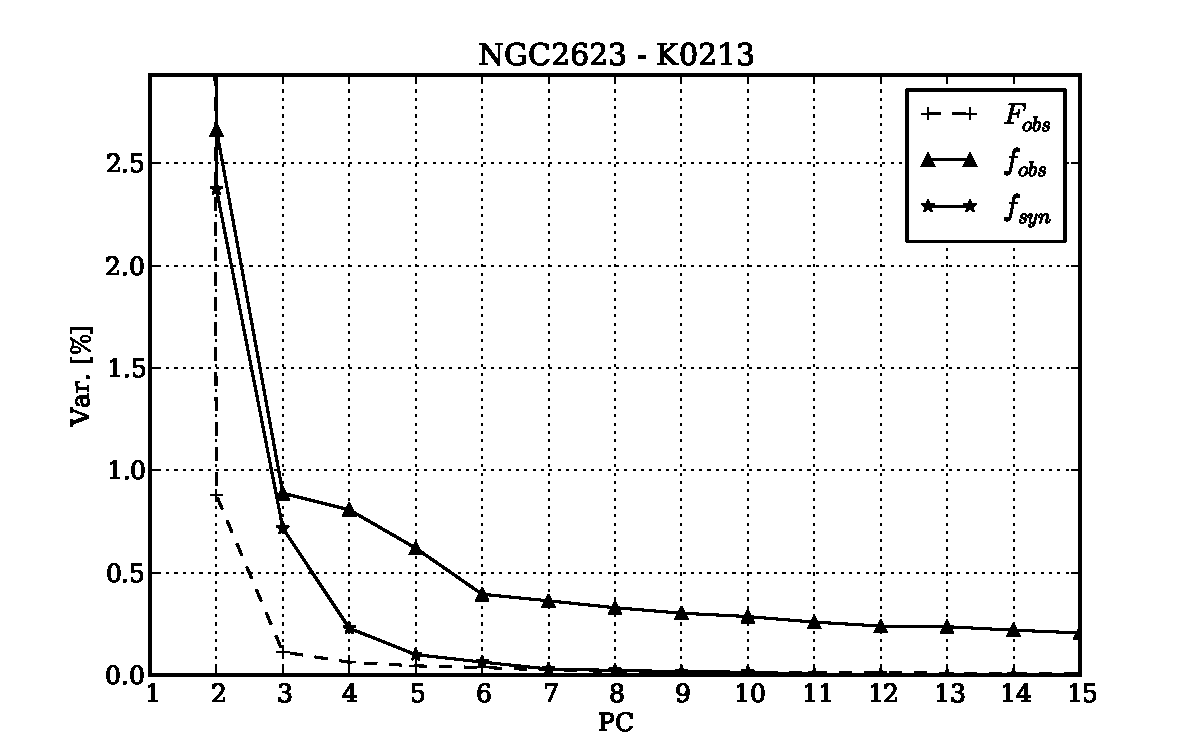
\includegraphics[height=0.33\textheight]{figuras/K0213-screetest.pdf}
    \caption[Scree test comparativo entre 3 PCAs - NGC 2623.]
    {Igual a Figura \ref{fig:K0008} para a galáxia NGC 2623.}
    \label{fig:K0213scree}
\end{figure}

\begin{figure}
    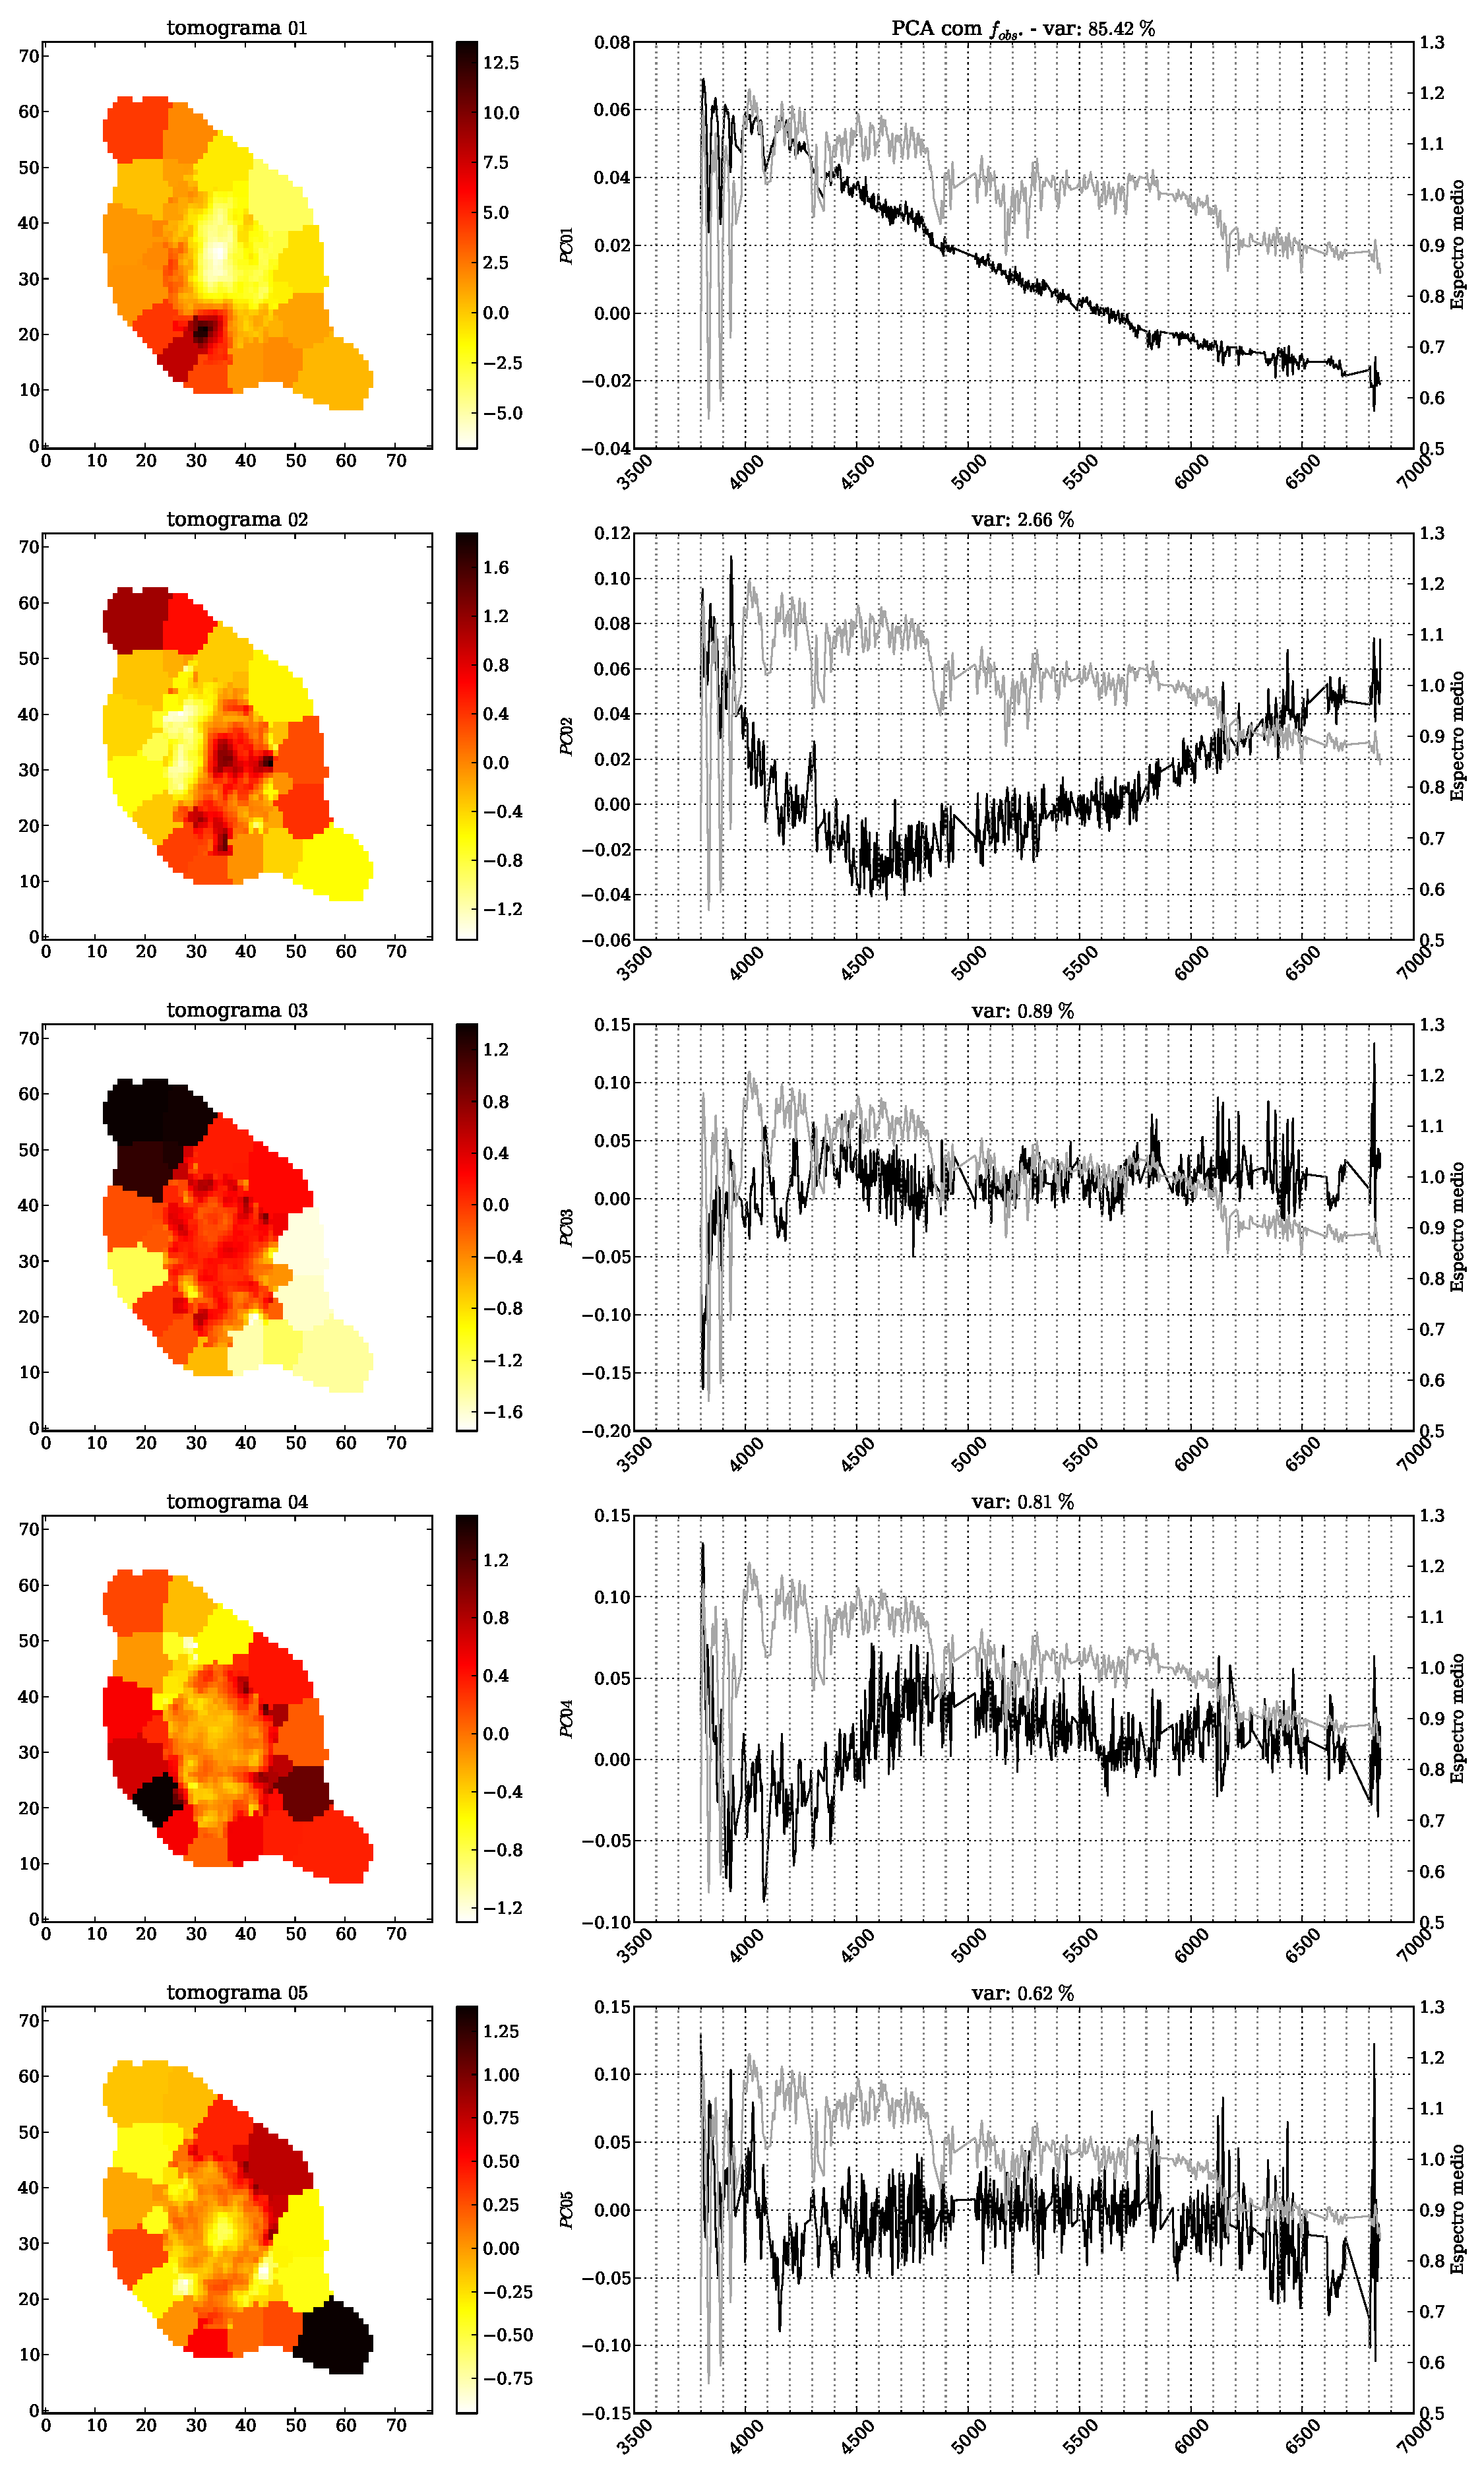
\includegraphics[width=0.85\textwidth]{figuras/K0213-tomo-obs-norm.pdf}
    \caption[Tomogramas de 1 a 5 para o cubo $F_{obs}$ norm. - NGC 2623.]
    {Igual a Figura \ref{fig:K0008tomofobsnorm} para a galáxia NGC 2623.}
    \label{fig:K0213tomofobsnorm}
\end{figure}

\begin{figure}
    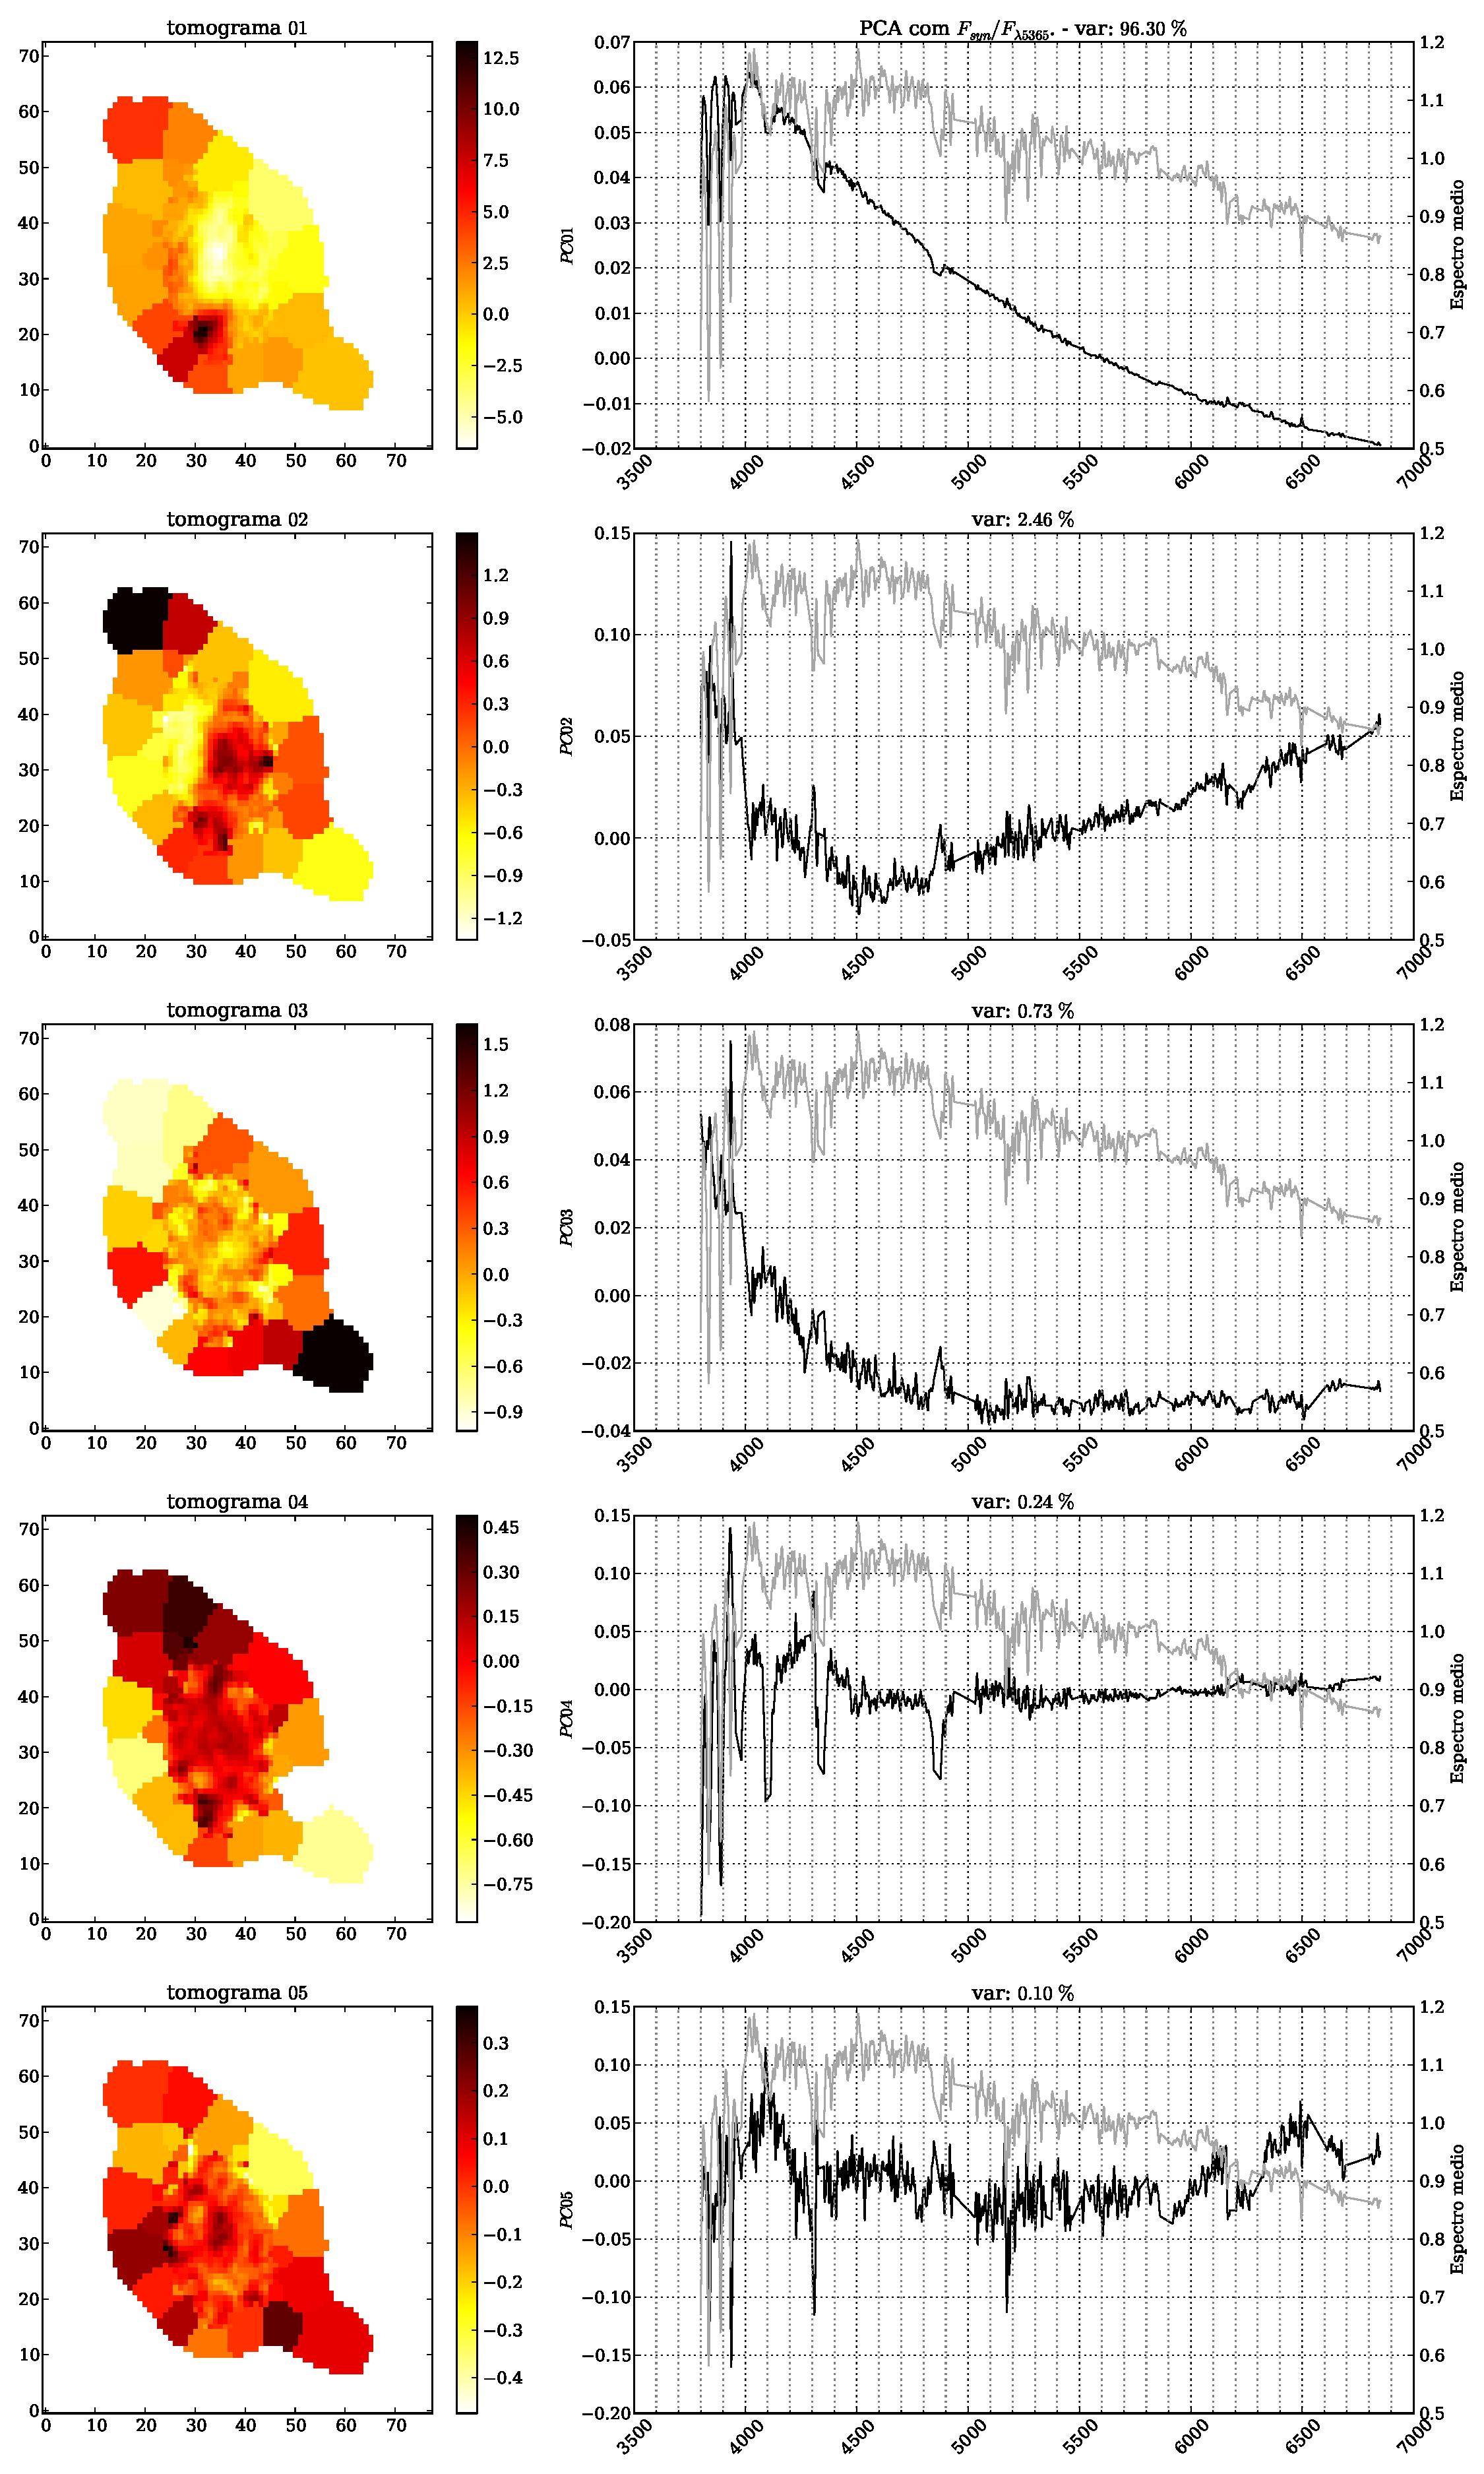
\includegraphics[width=0.85\textwidth]{figuras/K0213-tomo-syn-norm.pdf}
    \caption[Tomogramas de 1 a 5 para o cubo $F_{syn}$ norm. - NGC 2623.]
    {Igual a Figura \ref{fig:K0008tomofsynnorm} para a galáxia NGC 2623.}
    \label{fig:K0213tomofsynnorm}
\end{figure}

\begin{figure}
    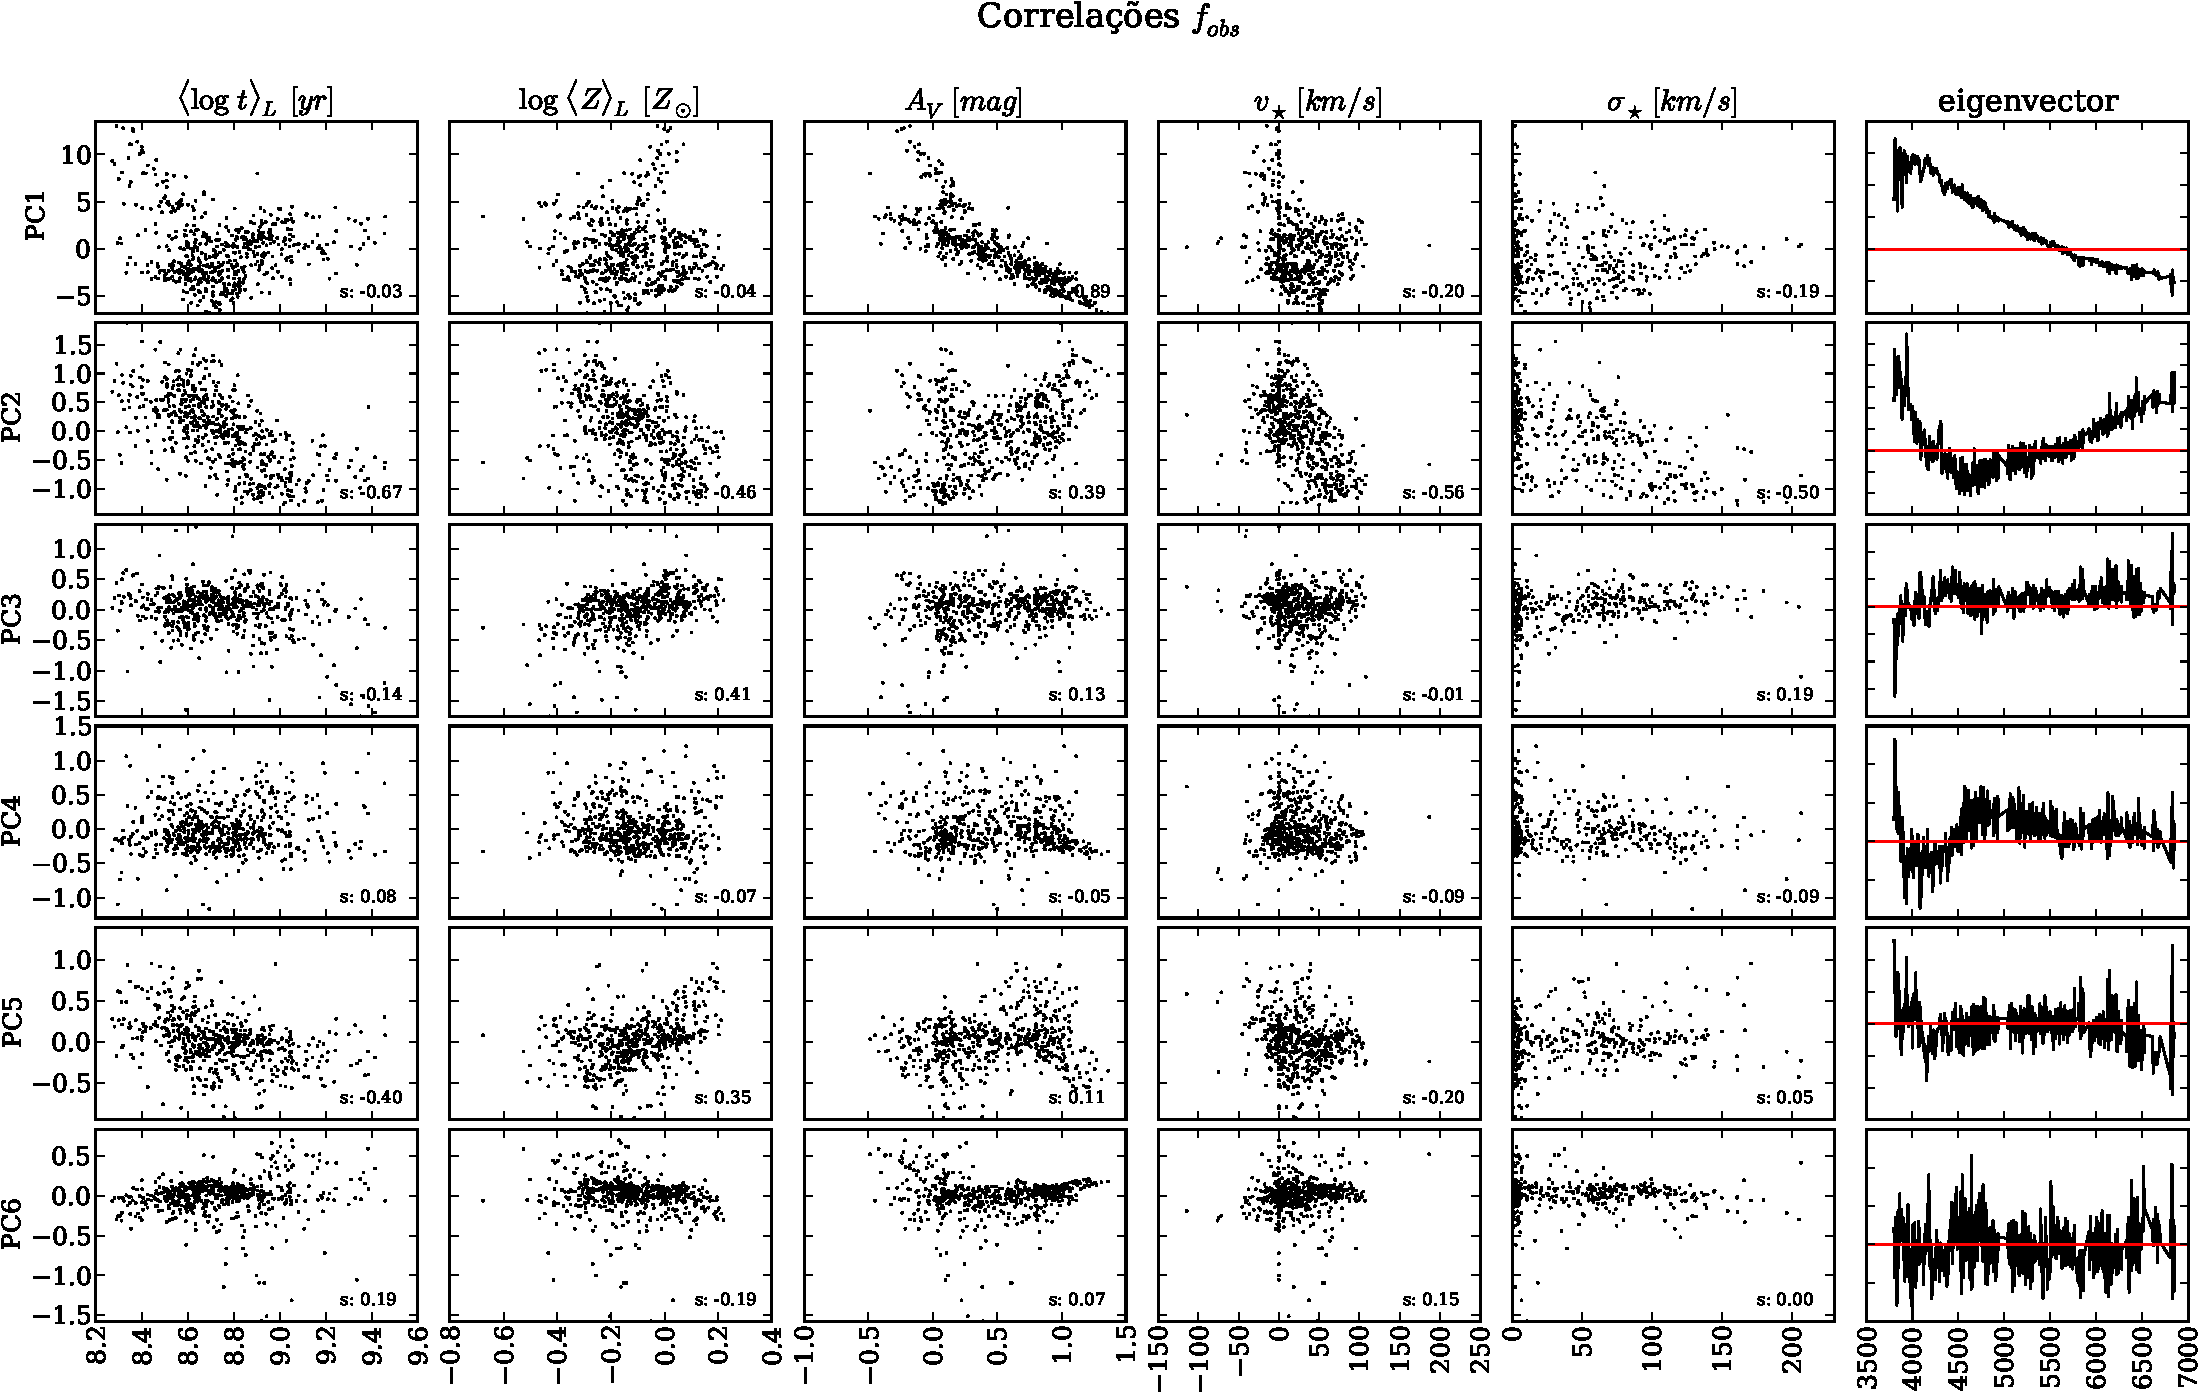
\includegraphics[width=1.3\textwidth, angle=-90]{figuras/K0213-correl-f_obs_norm-PCvsPhys.pdf}
	\caption[Correlações PCs vs. par\^ametros f\'isicos - $F_{obs}$ norm. - NGC 2623.]
	{Igual a Figura \ref{fig:K0008correfobsnorm} para a galáxia NGC 2623.}
    \label{fig:K0213correfobsnorm}
\end{figure}

\begin{figure}
    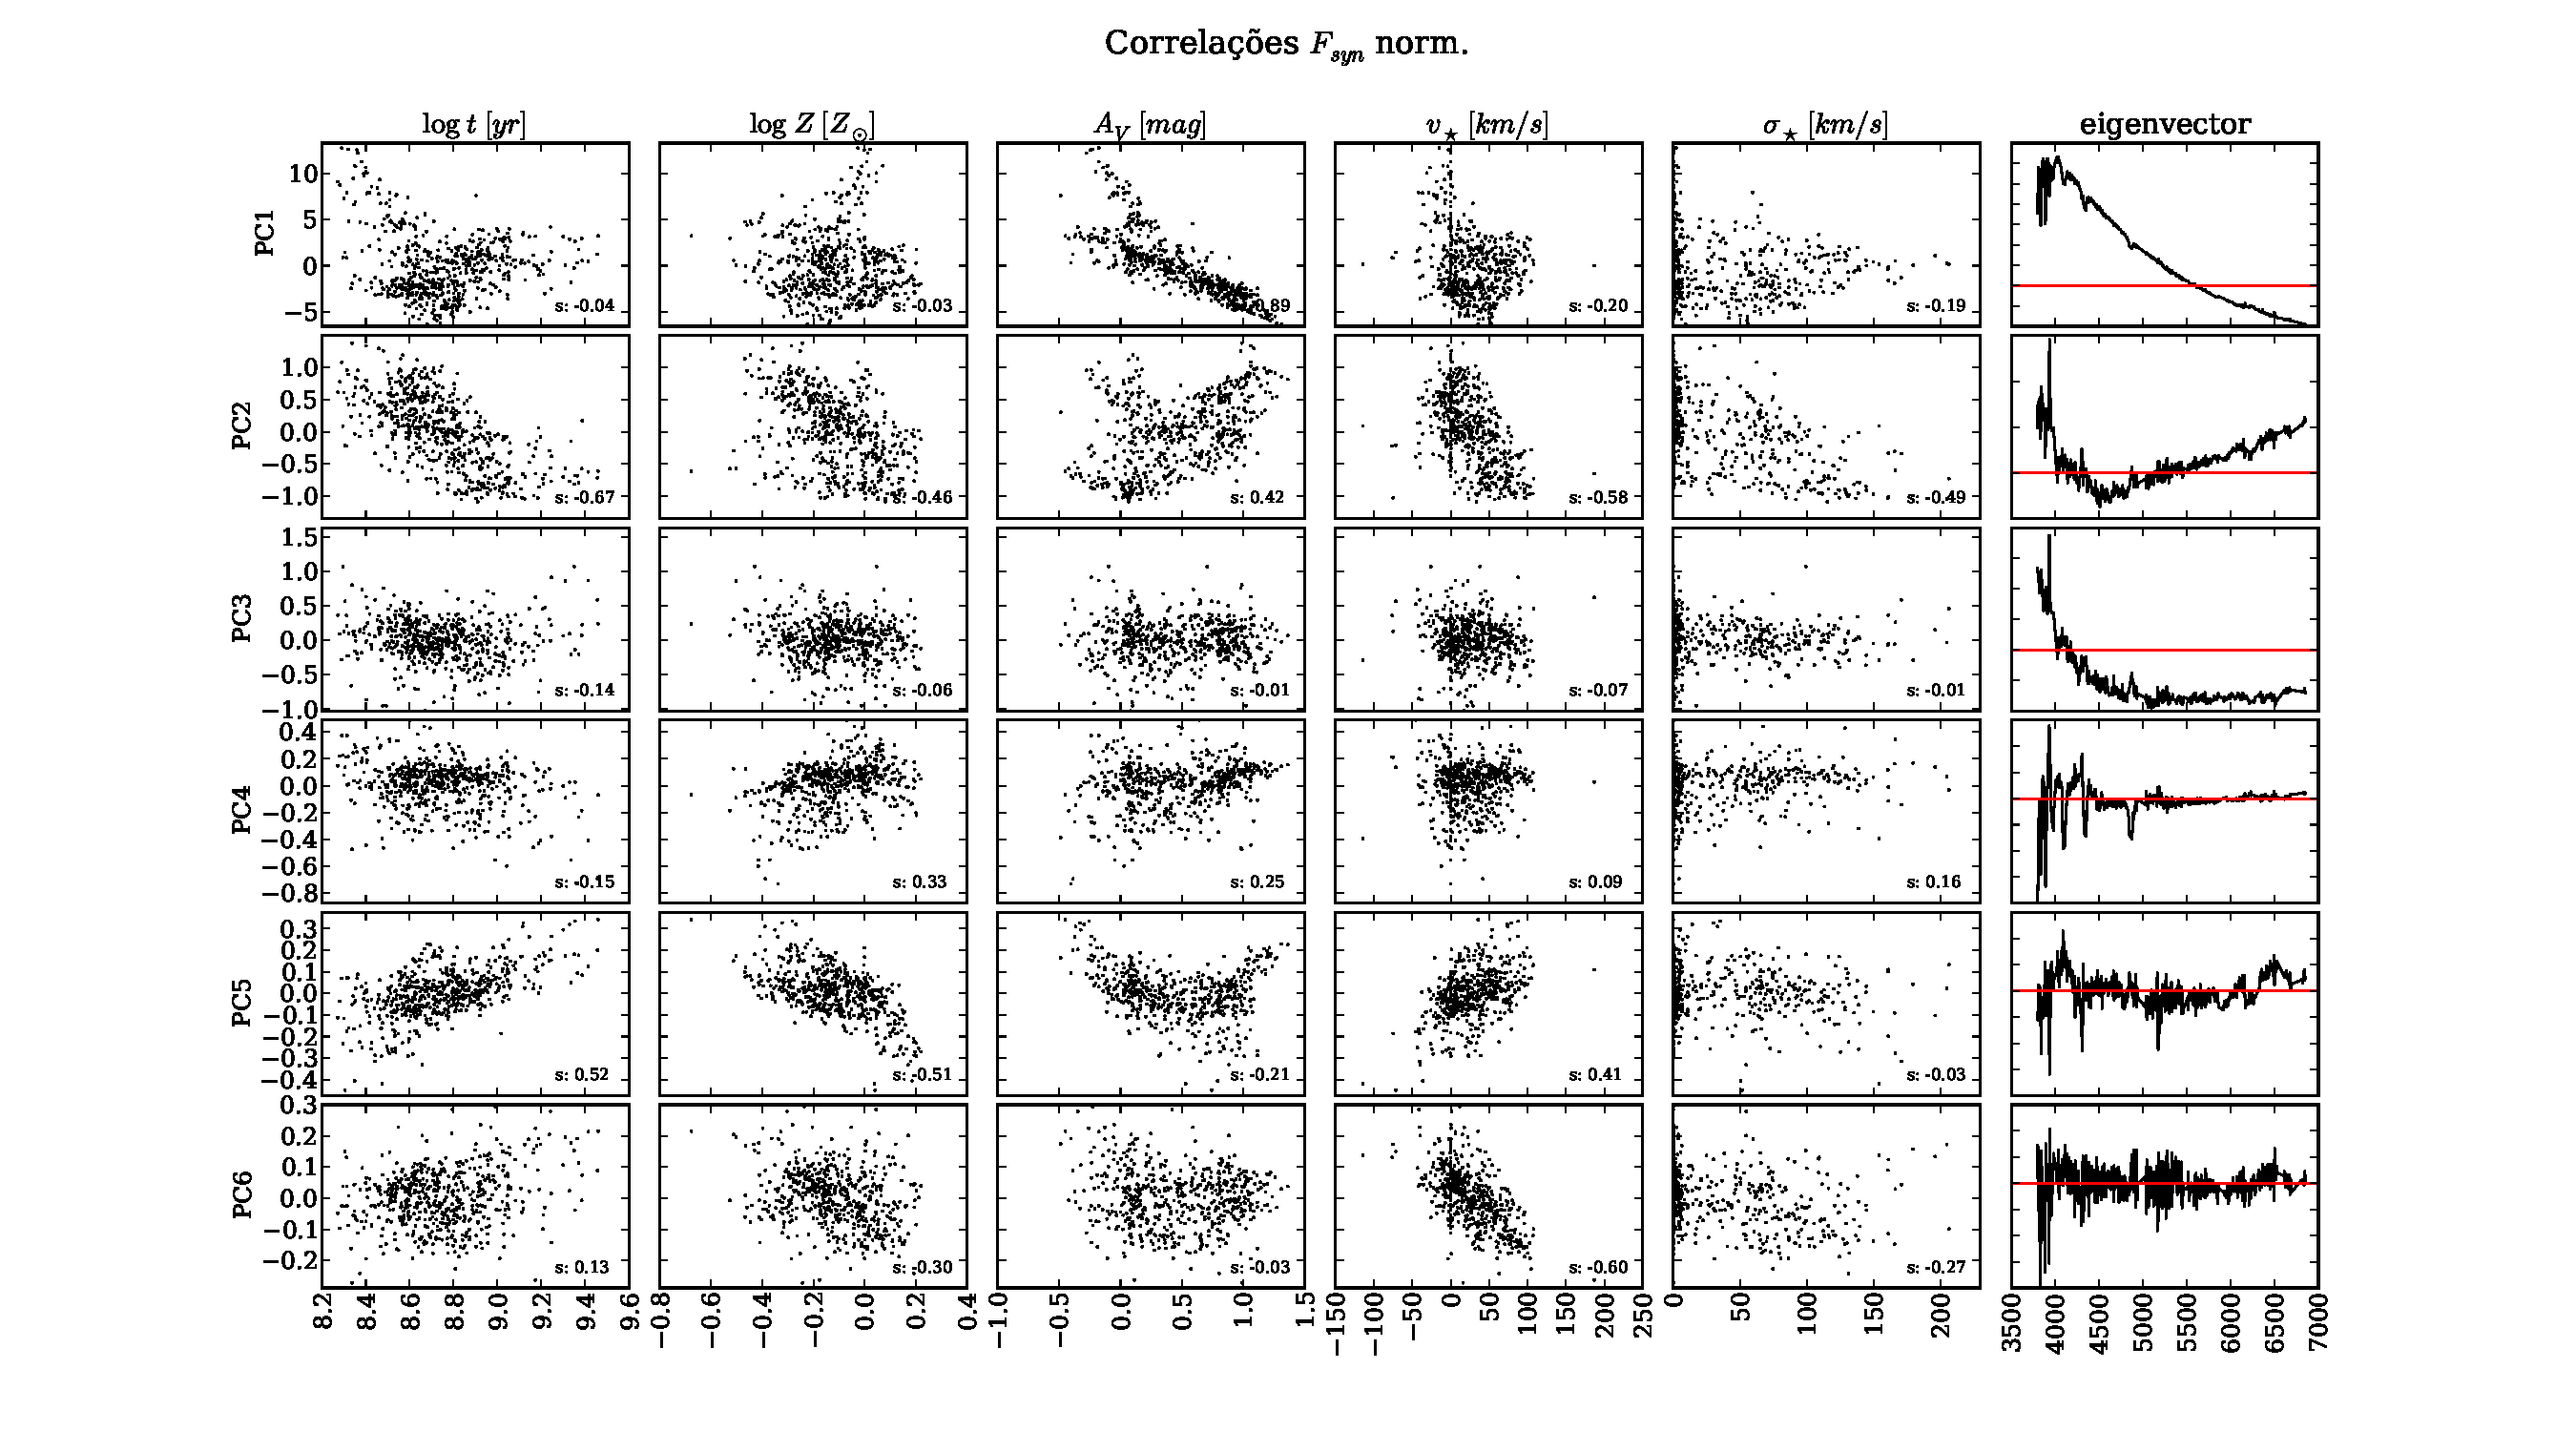
\includegraphics[width=1.3\textwidth, angle=-90]{figuras/K0213-correl-f_syn_norm-PCvsPhys.pdf}
	\caption[Correlações PCs vs. par\^ametros f\'isicos - $F_{syn}$ norm. - NGC 2623.]
	{Igual a Figura \ref{fig:K0008correfsynnorm} para a galáxia NGC 2623.}
    \label{fig:K0213correfsynnorm}
\end{figure}

\subsection{ARP 220 - CALIFA 802}

\begin{figure}
    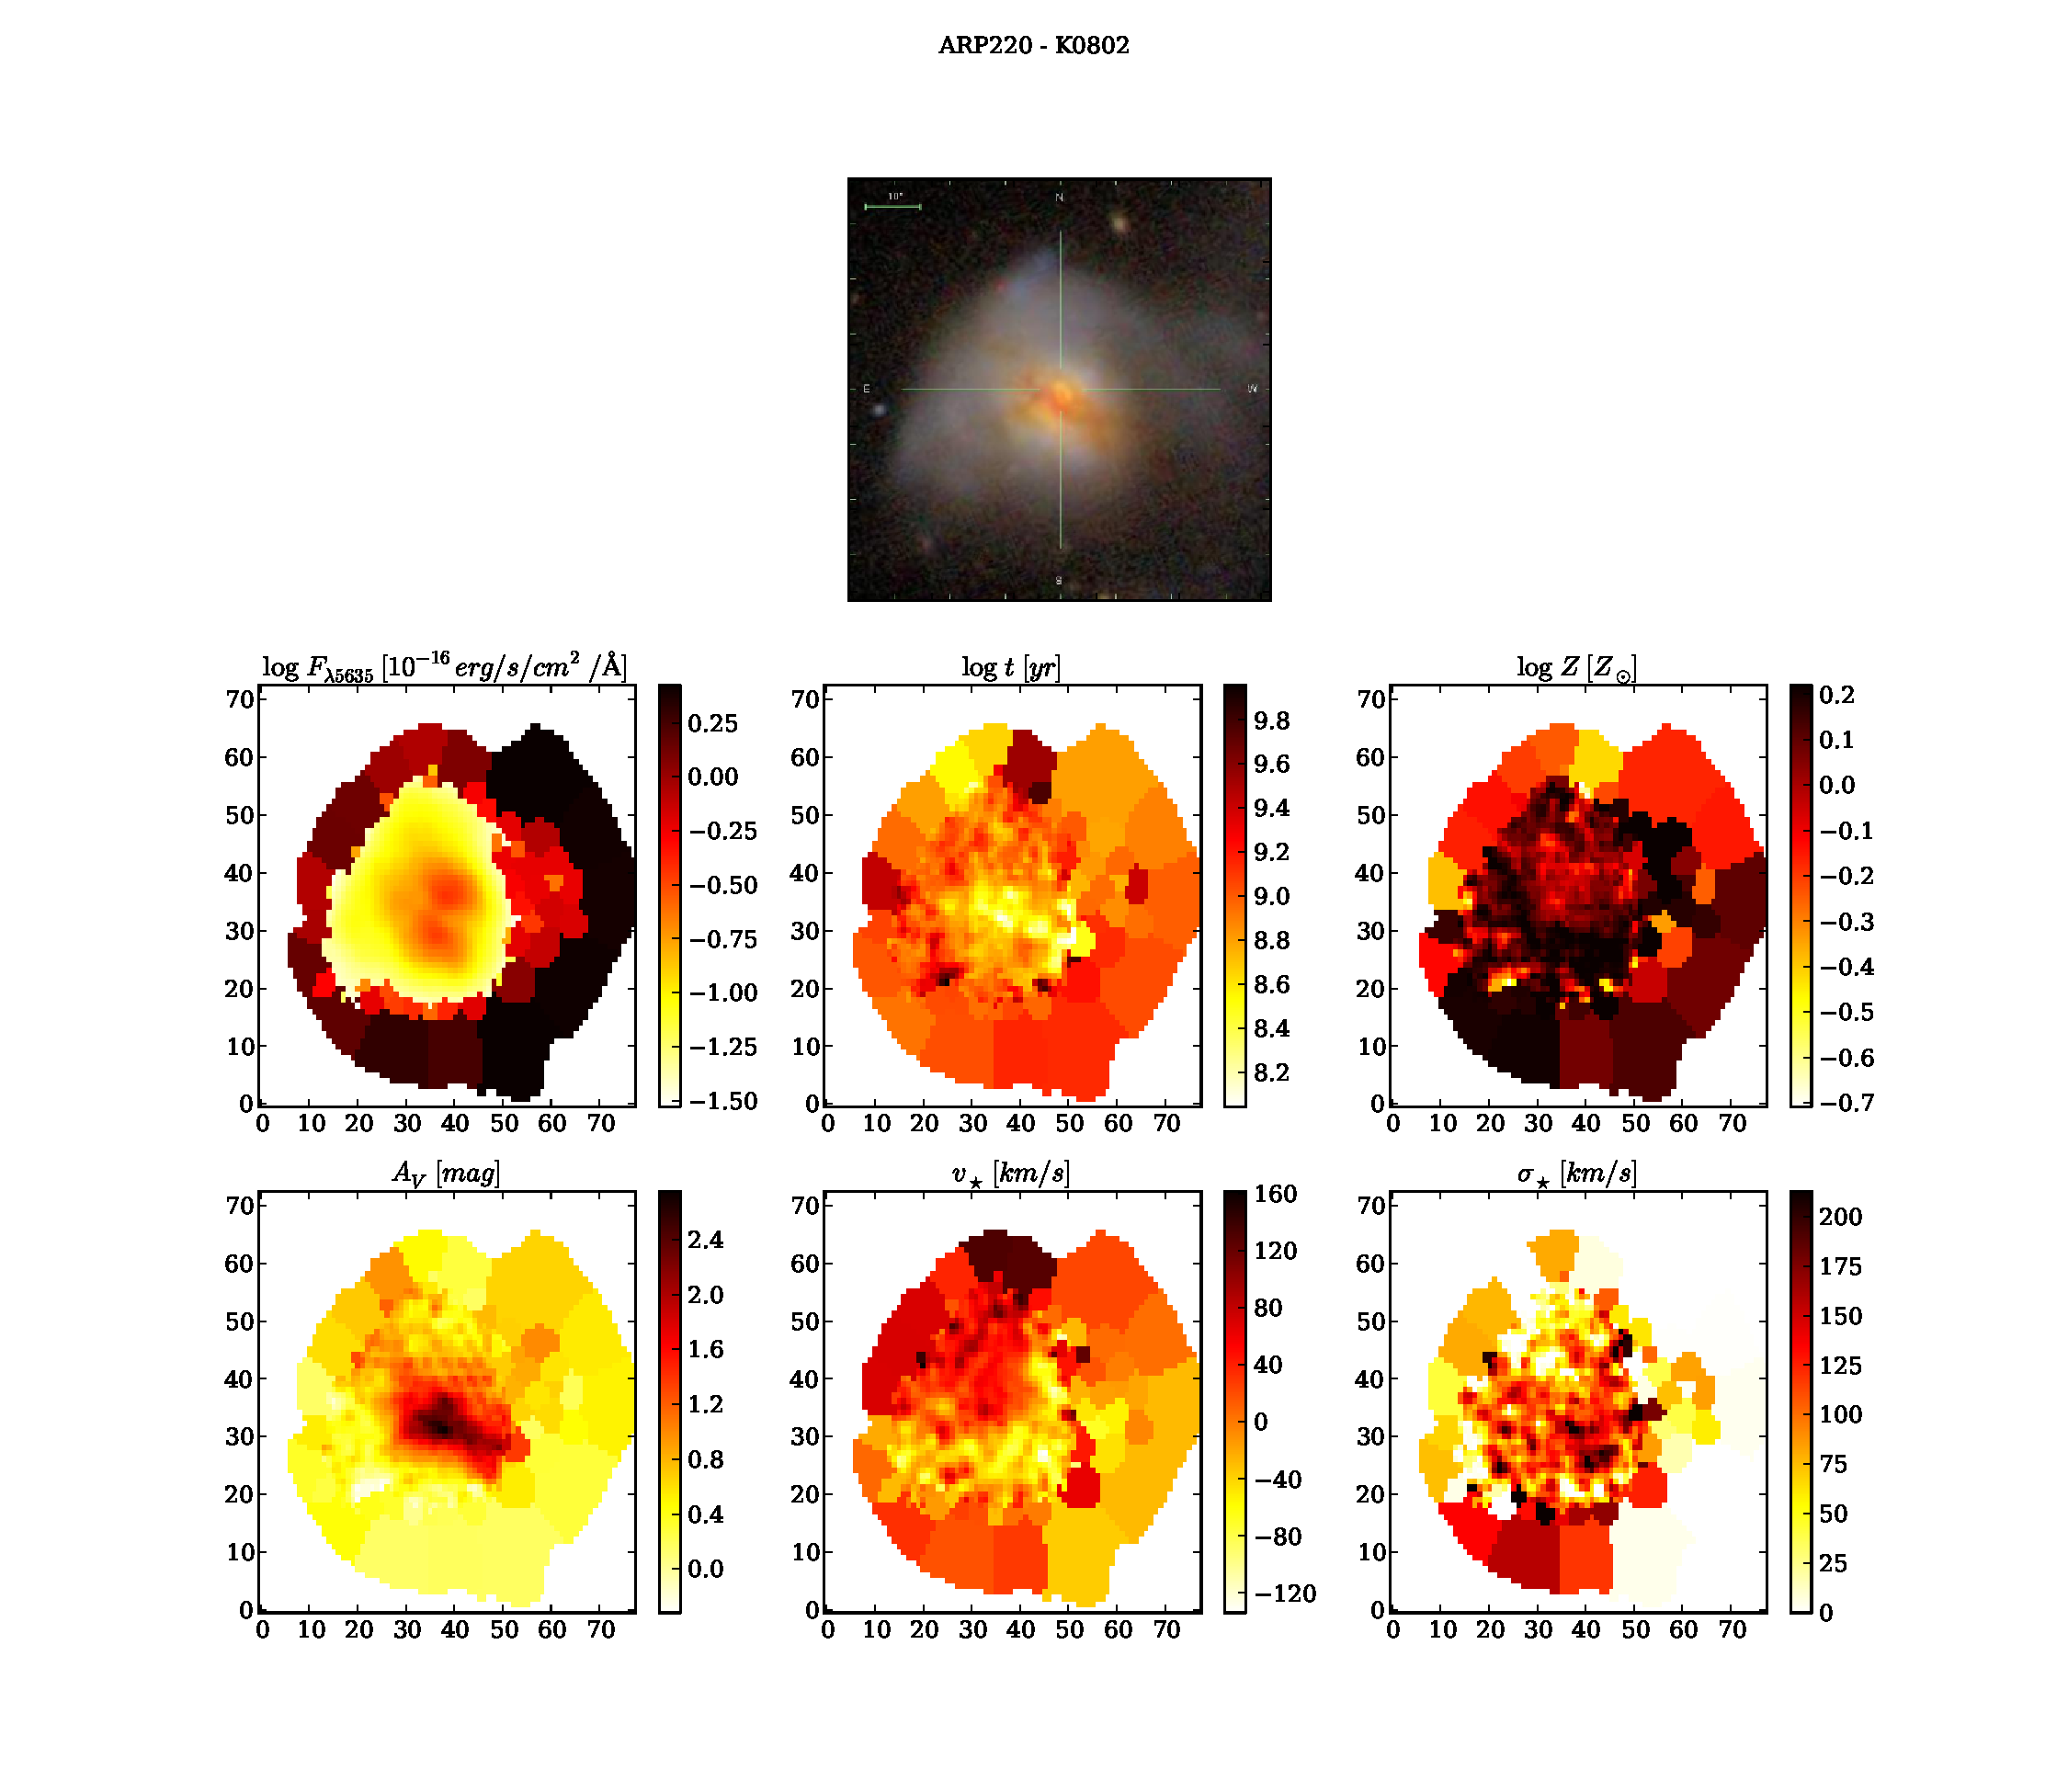
\includegraphics[width=1.\textwidth]{figuras/K0802-apresent.pdf}
    \caption[Propriedades f\'isicas da gal\'axia ARP 220.]
    {Igual a Figura \ref{fig:K0008apresent} para a galáxia ARP 220.}
    \label{fig:K0802apresent}
\end{figure}

\begin{figure}
    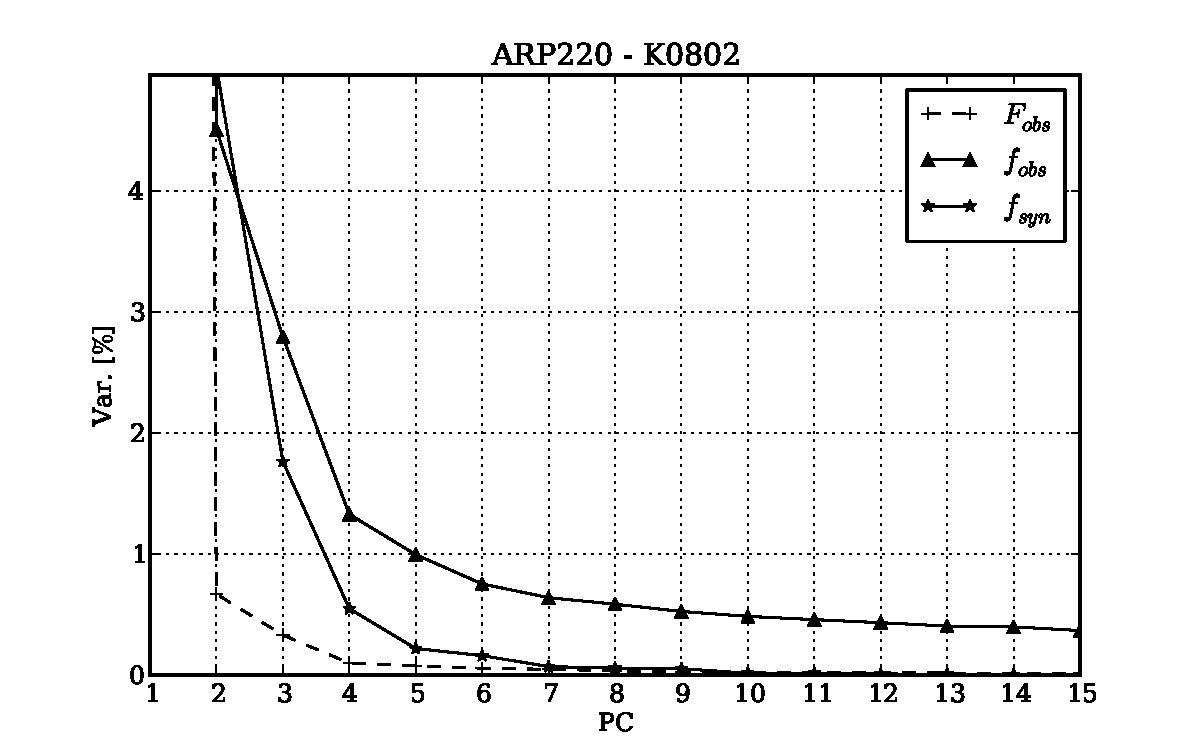
\includegraphics[height=0.33\textheight]{figuras/K0802-screetest.pdf}
    \caption[Scree test comparativo entre 3 PCAs - ARP 220.]
	{Igual a Figura \ref{fig:K0008} para a galáxia ARP 220.}
    \label{fig:K0802scree}
\end{figure}

\begin{figure}
    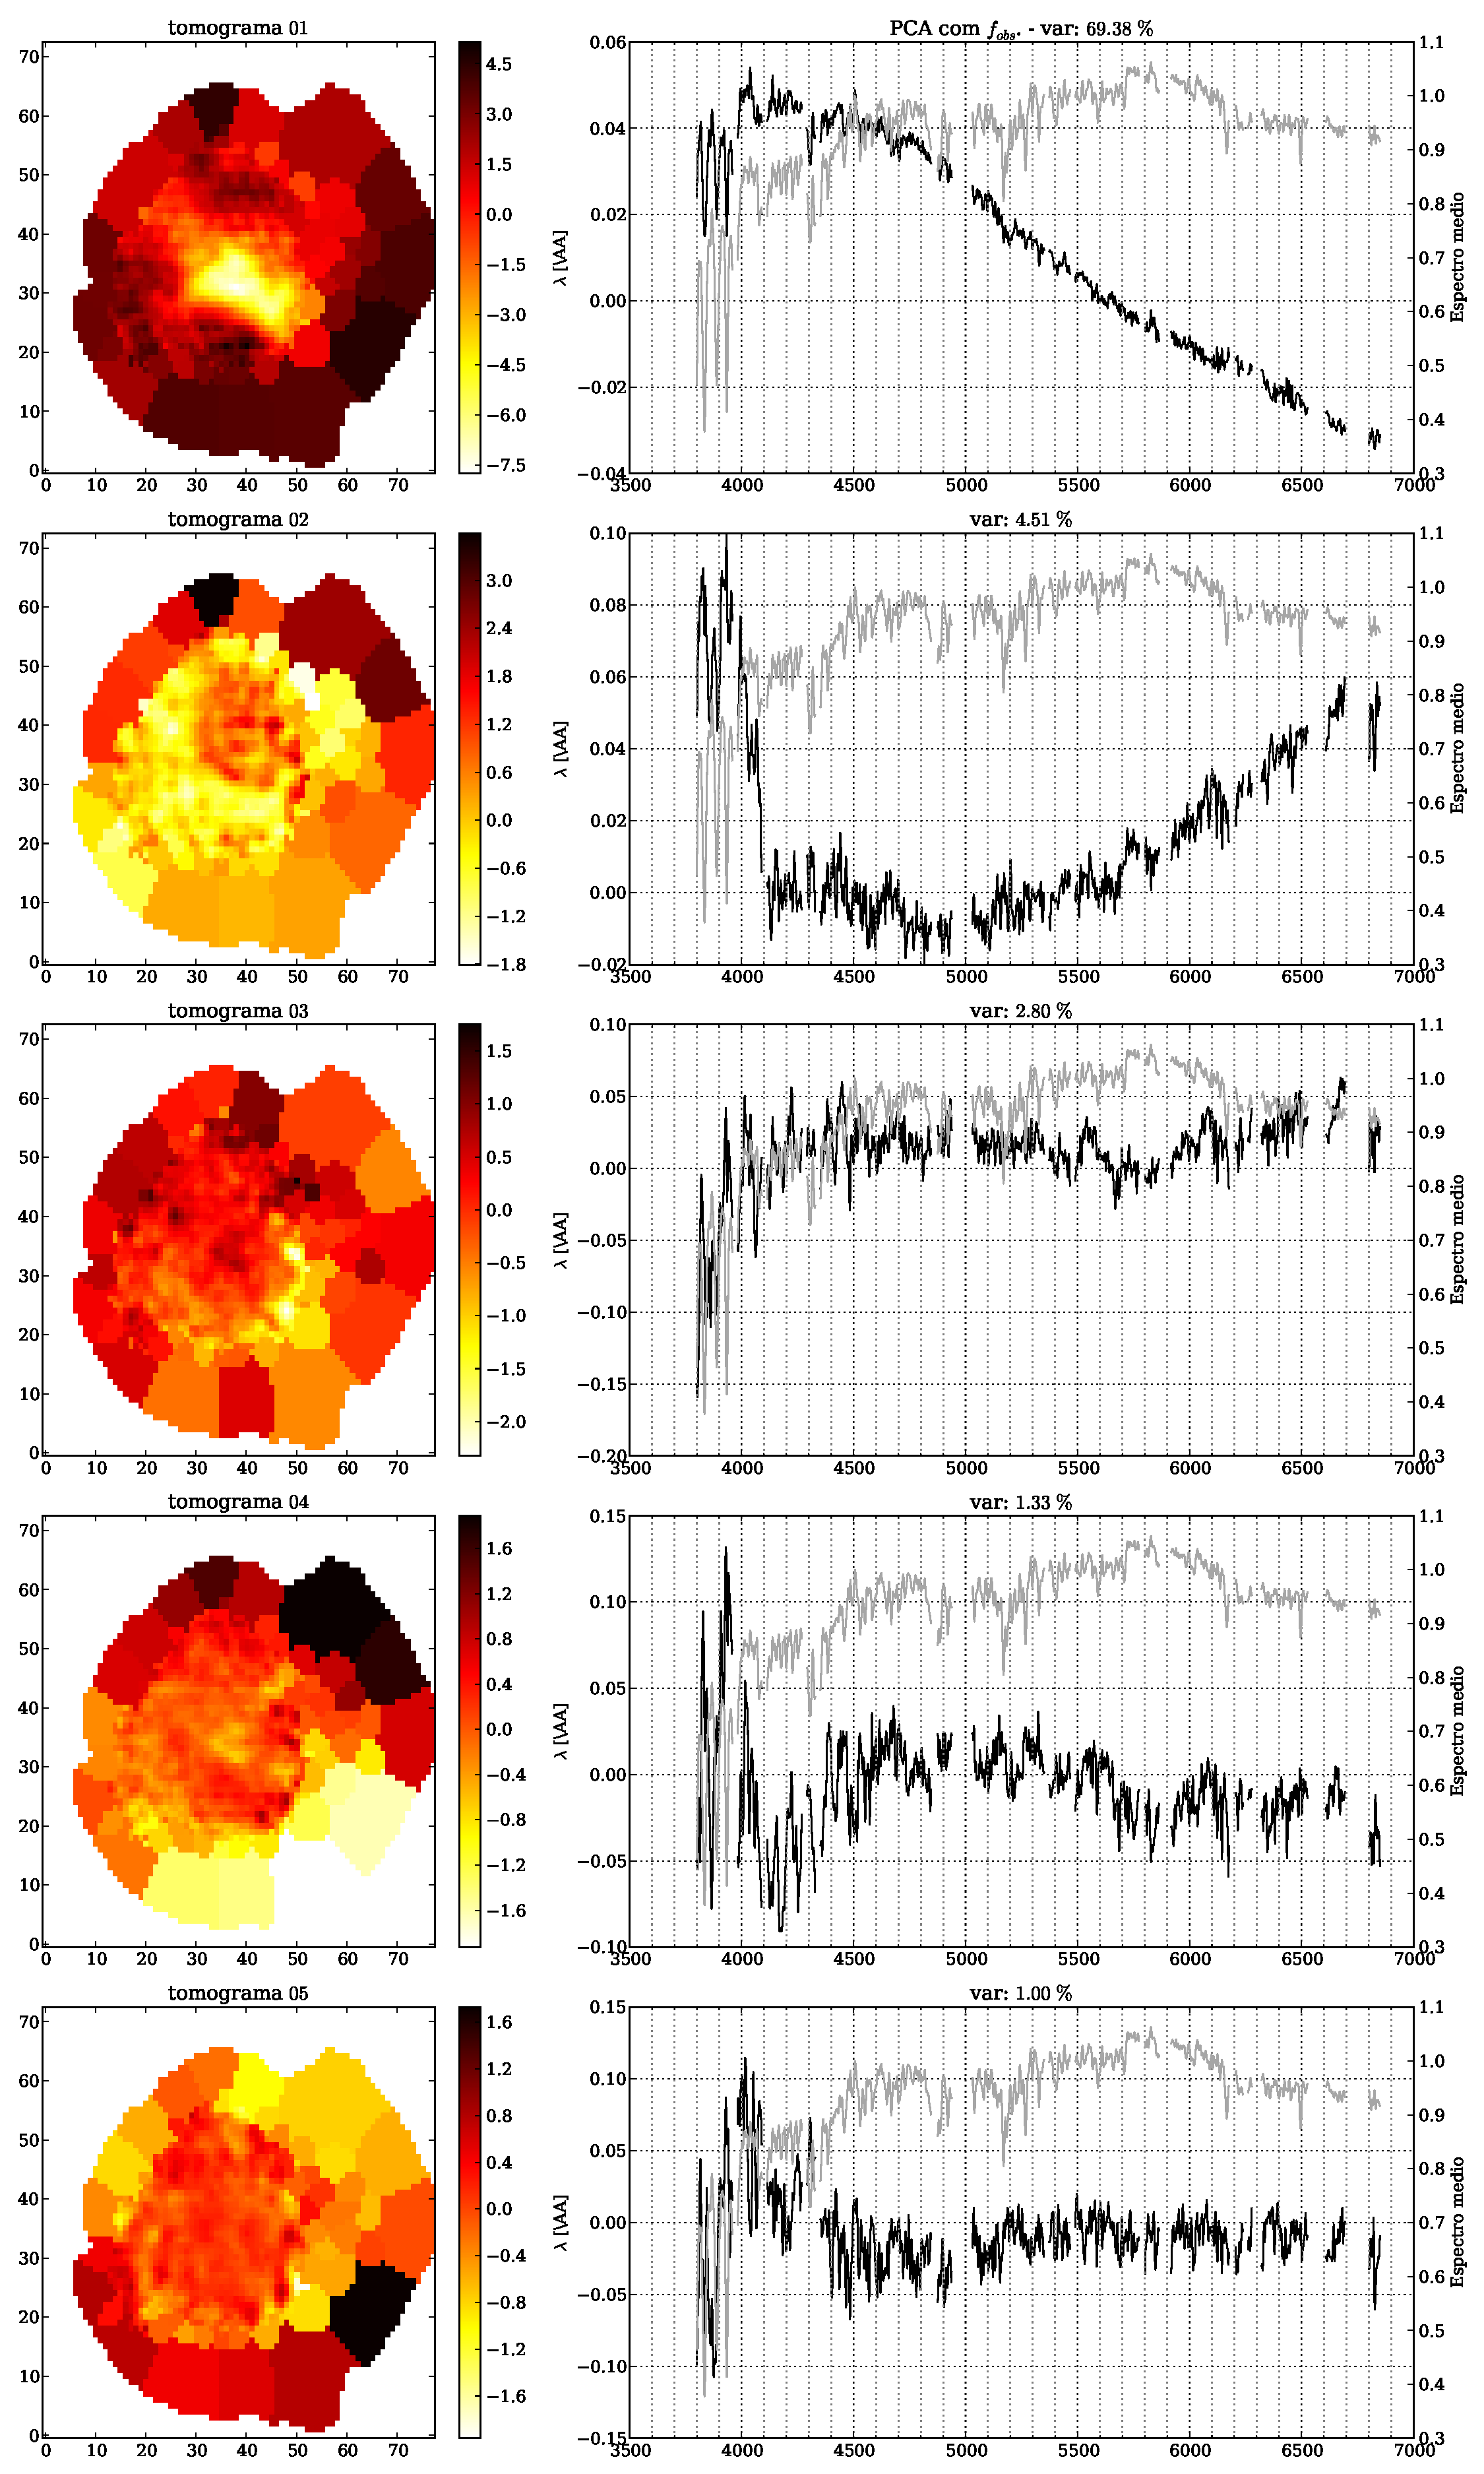
\includegraphics[width=0.85\textwidth]{figuras/K0802-tomo-obs-norm.pdf}
    \caption[Tomogramas de 1 a 5 para o cubo $F_{obs}$ norm. - ARP 220.]
    {Igual a Figura \ref{fig:K0008tomofobsnorm} para a galáxia ARP 220.}
    \label{fig:K0802tomofobsnorm}
\end{figure}

\begin{figure}
    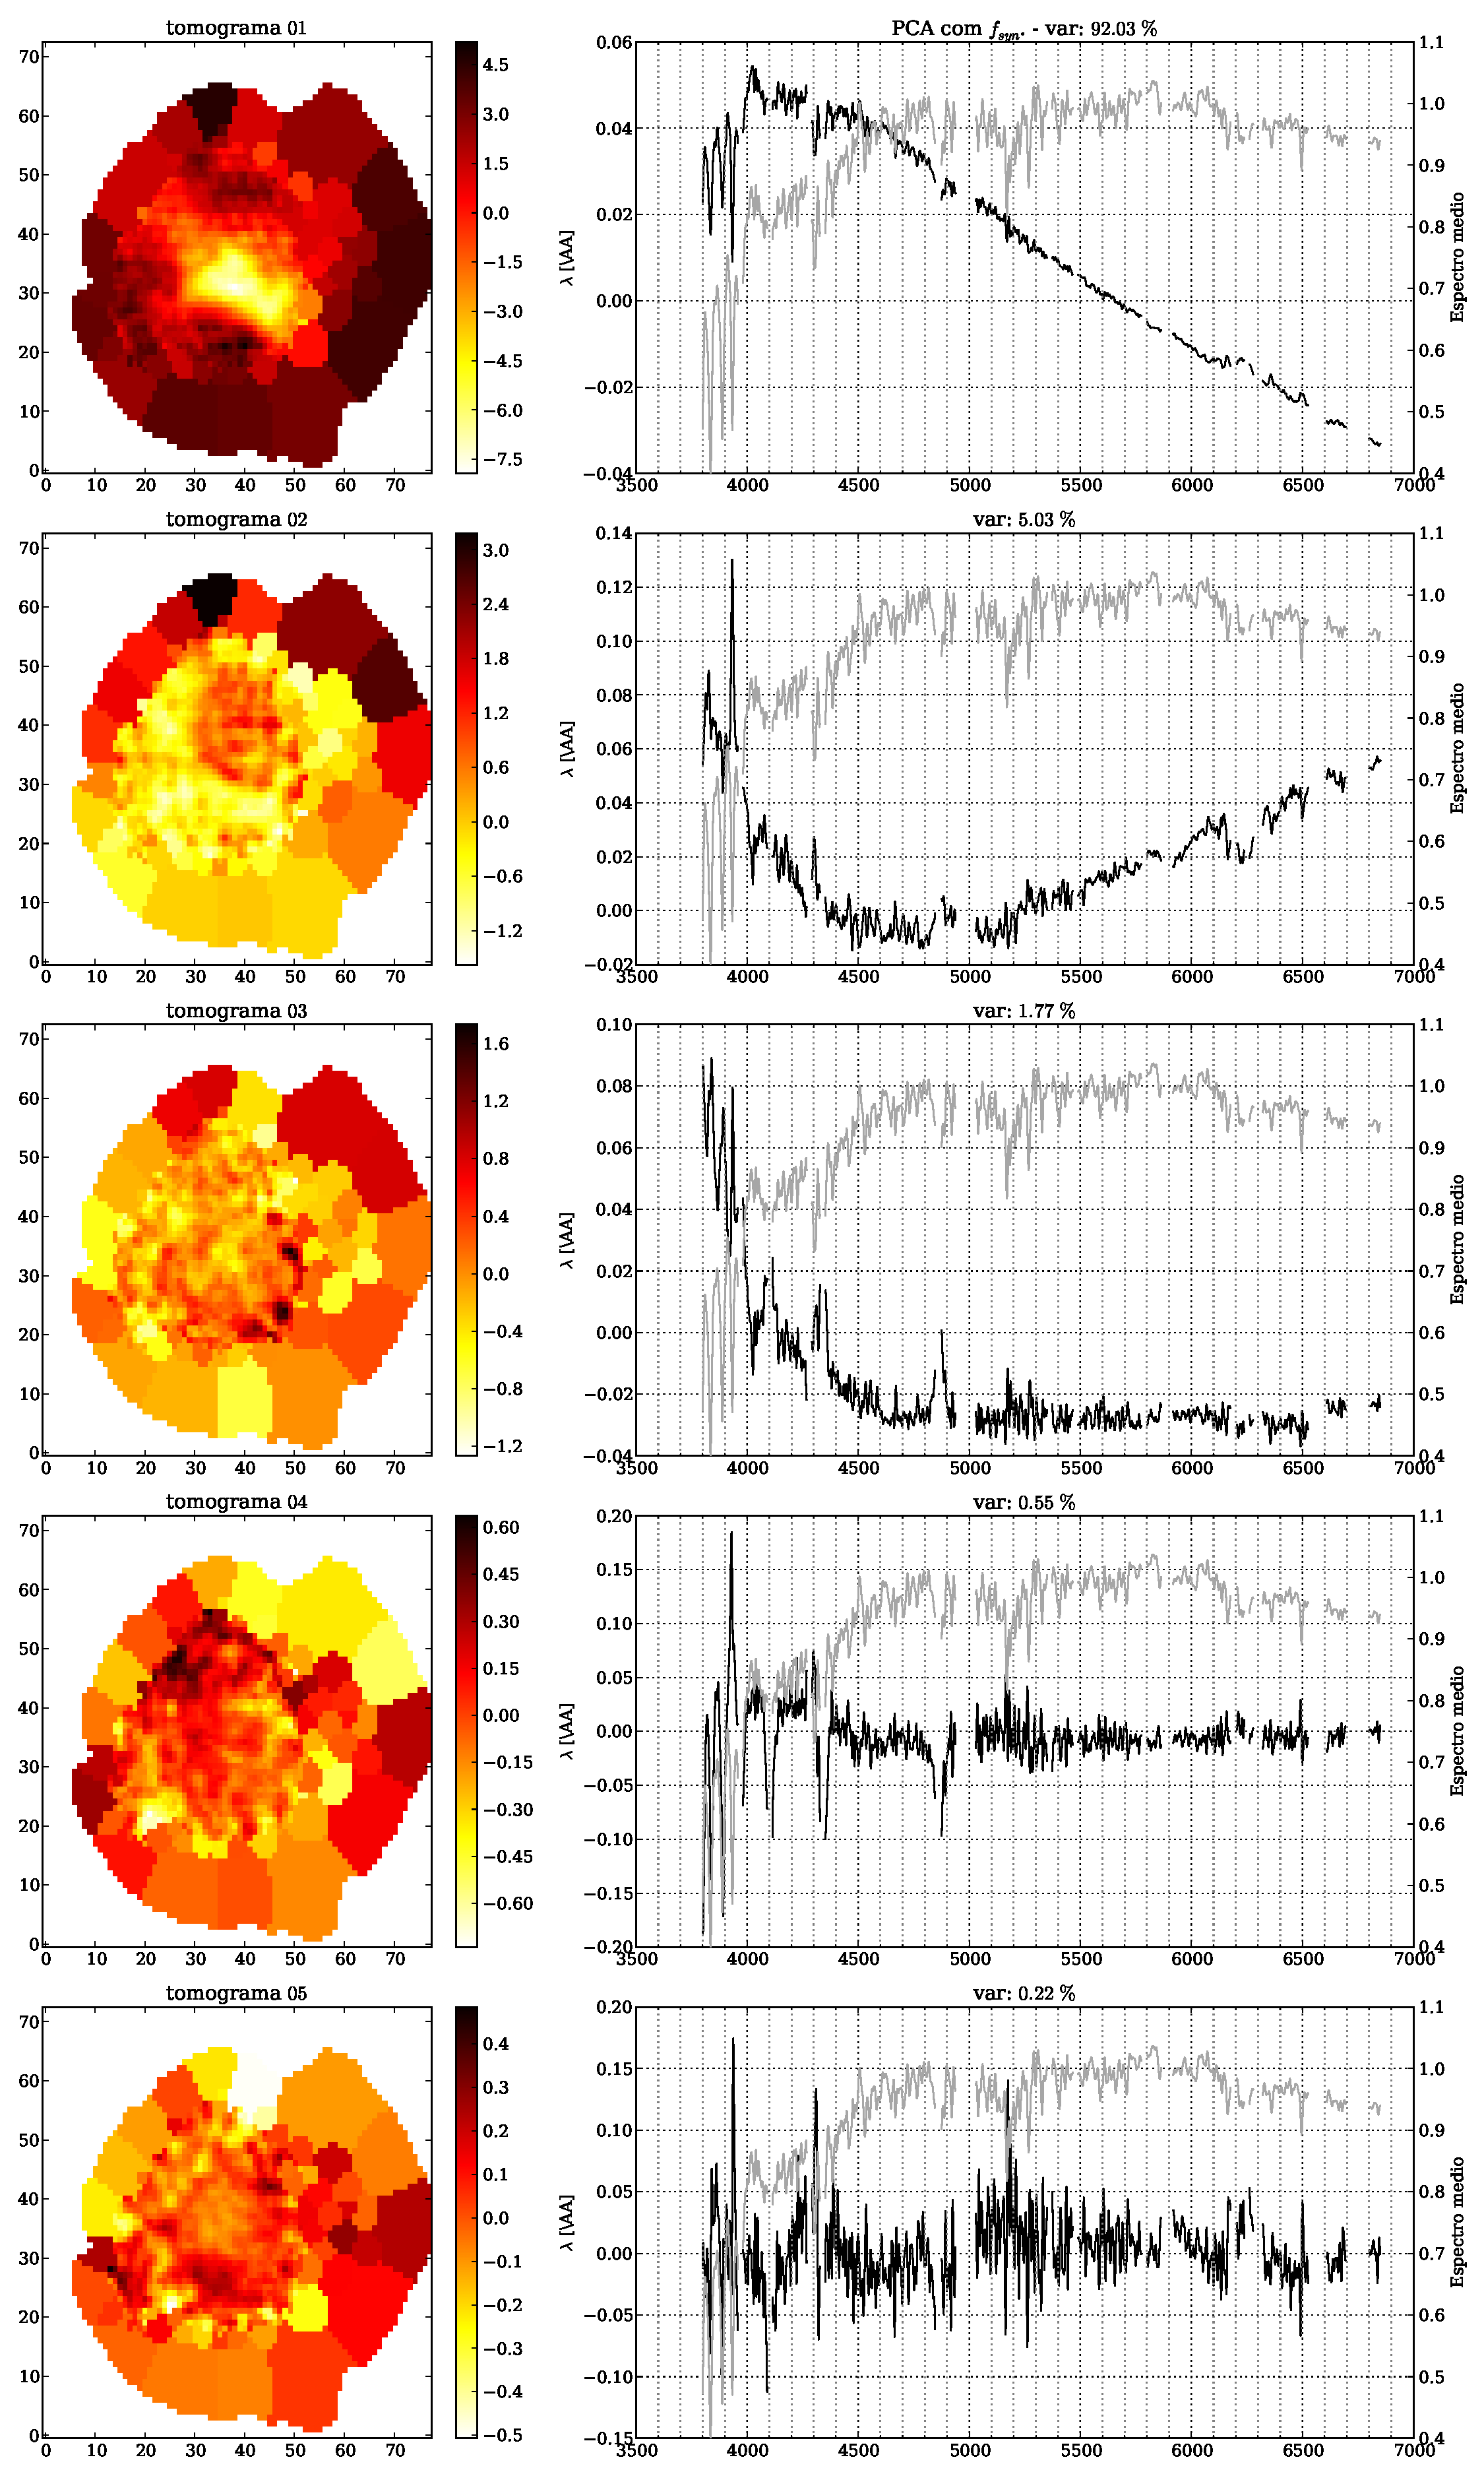
\includegraphics[width=0.85\textwidth]{figuras/K0802-tomo-syn-norm.pdf}
    \caption[Tomogramas de 1 a 5 para o cubo $F_{obs}$ norm. - ARP 220.]
    {Igual a Figura \ref{fig:K0008tomofsynnorm} para a galáxia ARP 220.}
    \label{fig:K0802tomofsynnorm}
\end{figure}

\begin{figure}
    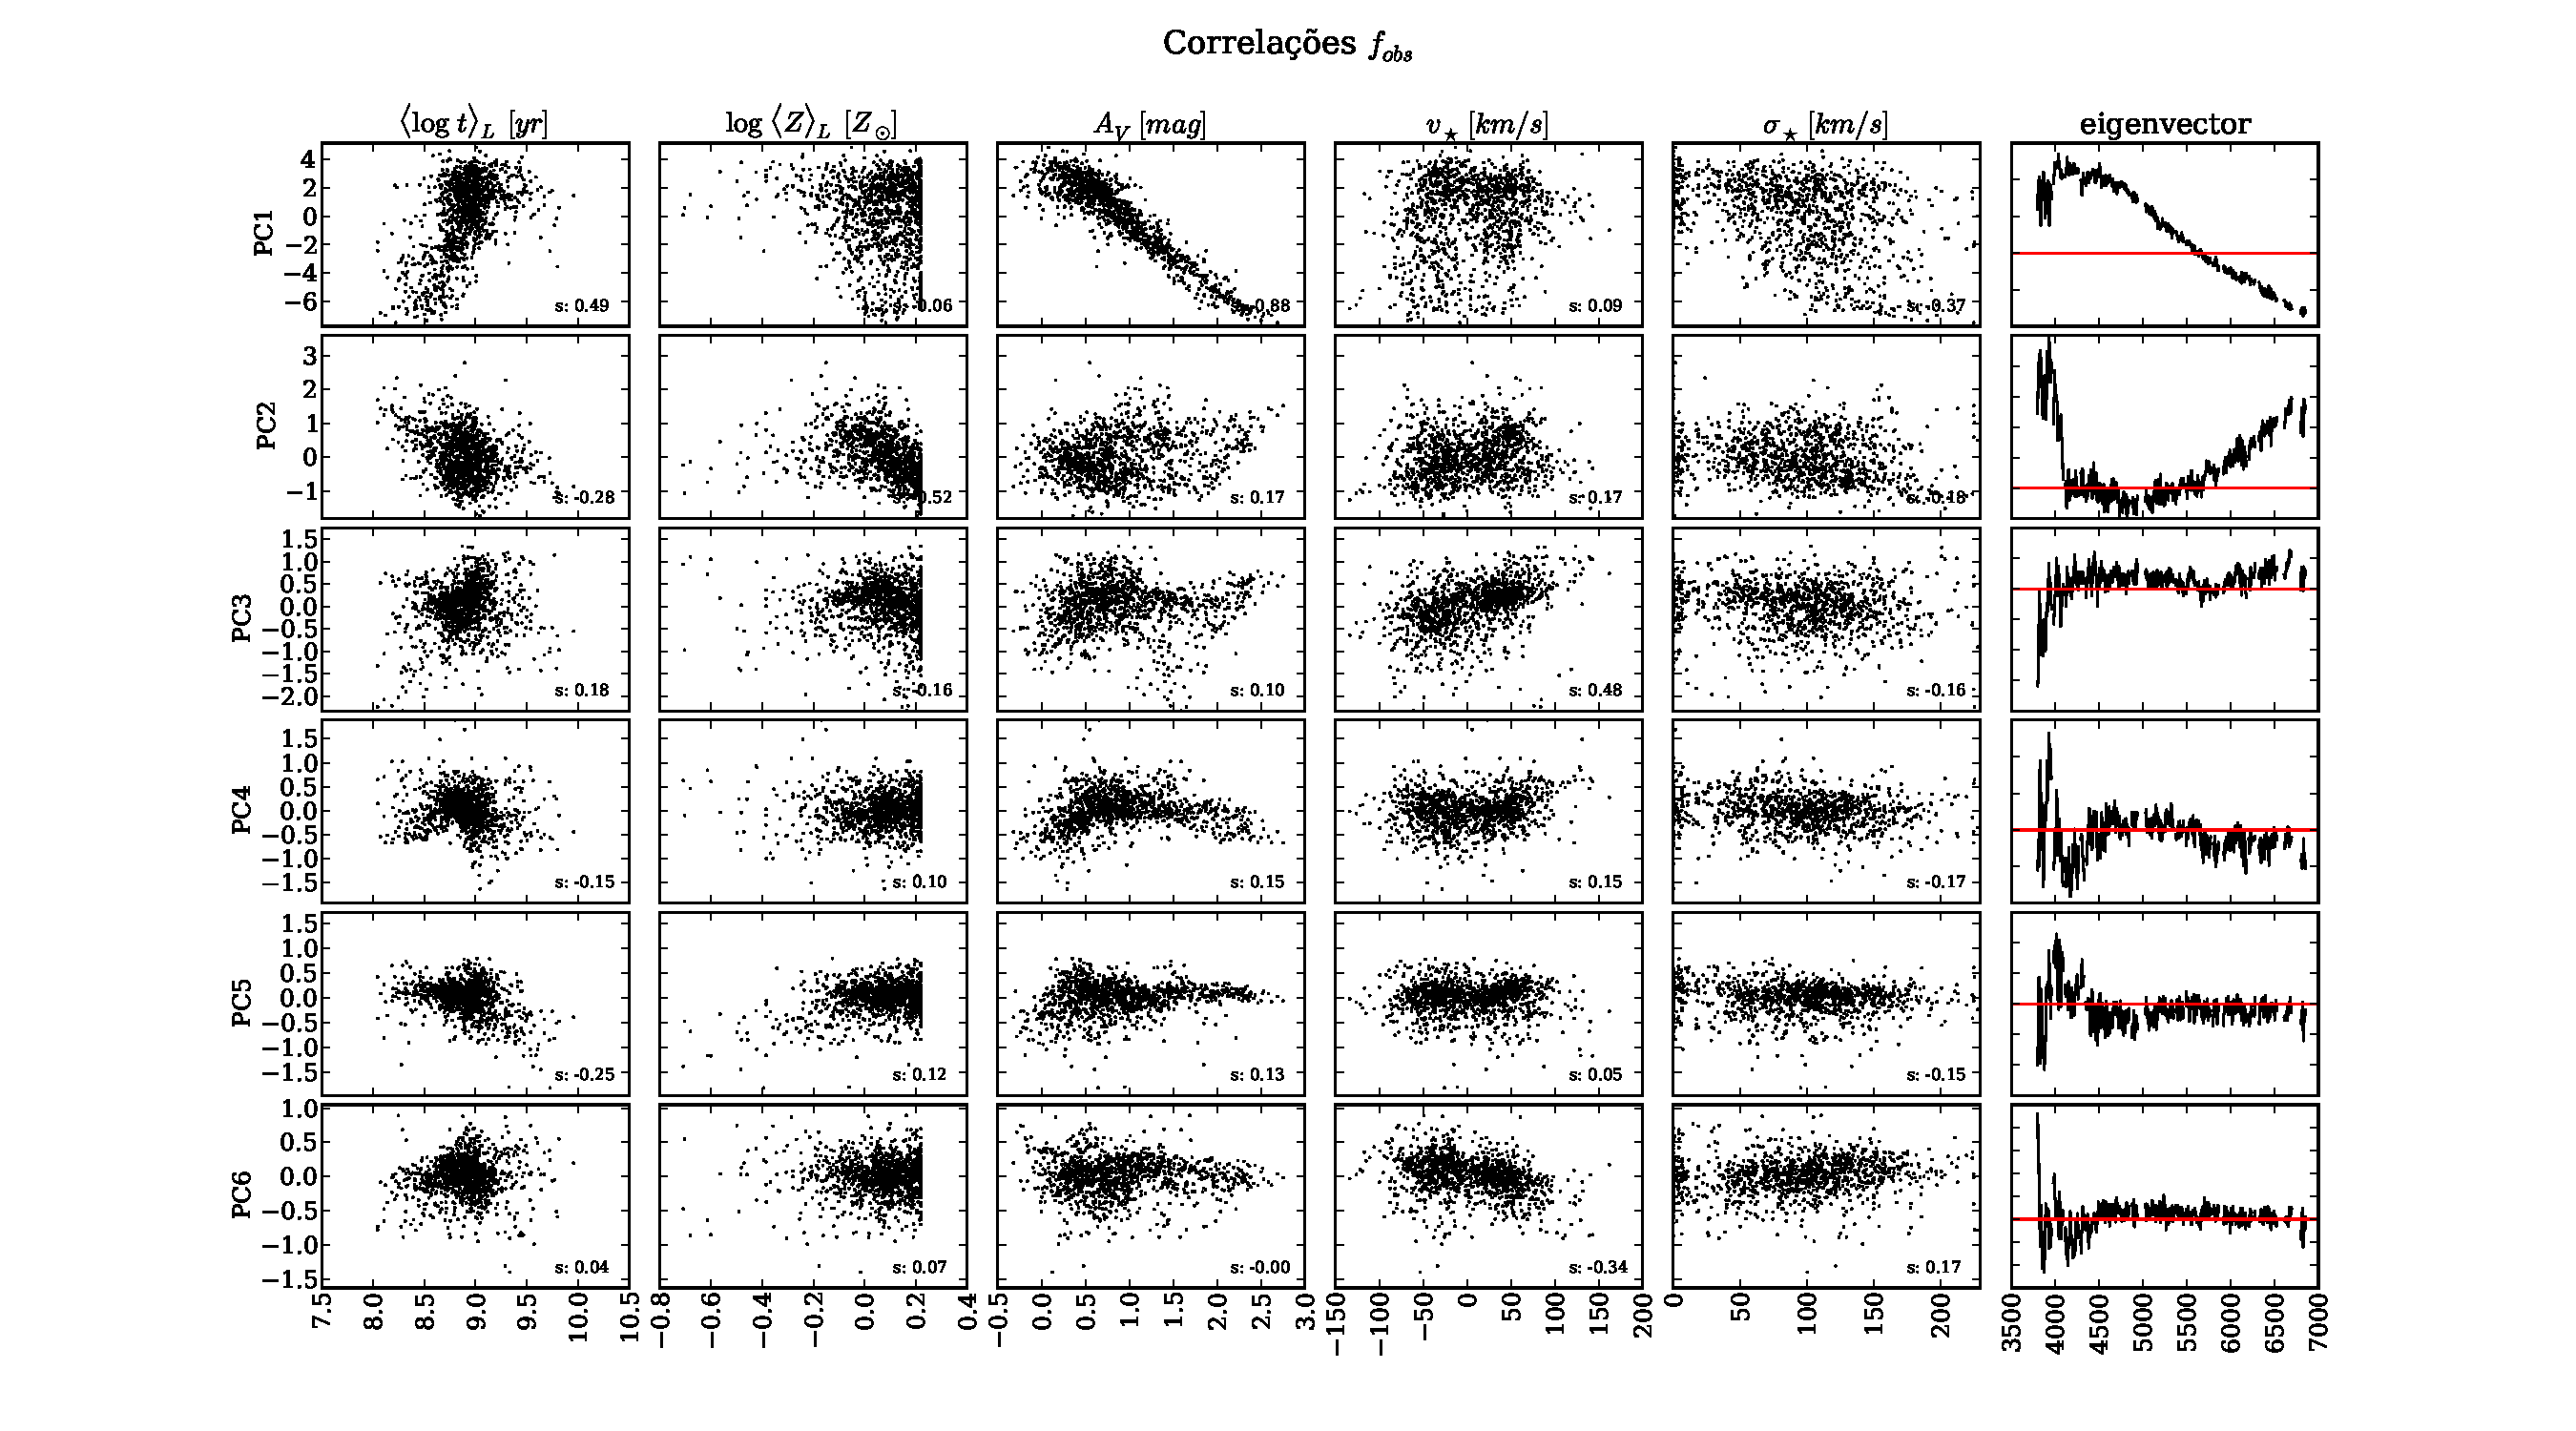
\includegraphics[width=1.3\textwidth, angle=-90]{figuras/K0802-correl-f_obs_norm-PCvsPhys.pdf}
	\caption[Correlações PCs vs. par\^ametros f\'isicos - $F_{obs}$ norm. - ARP 220.]
	{Igual a Figura \ref{fig:K0008correfobsnorm} para a galáxia ARP 220.}
    \label{fig:K0802correfobsnorm}
\end{figure}

\begin{figure}
    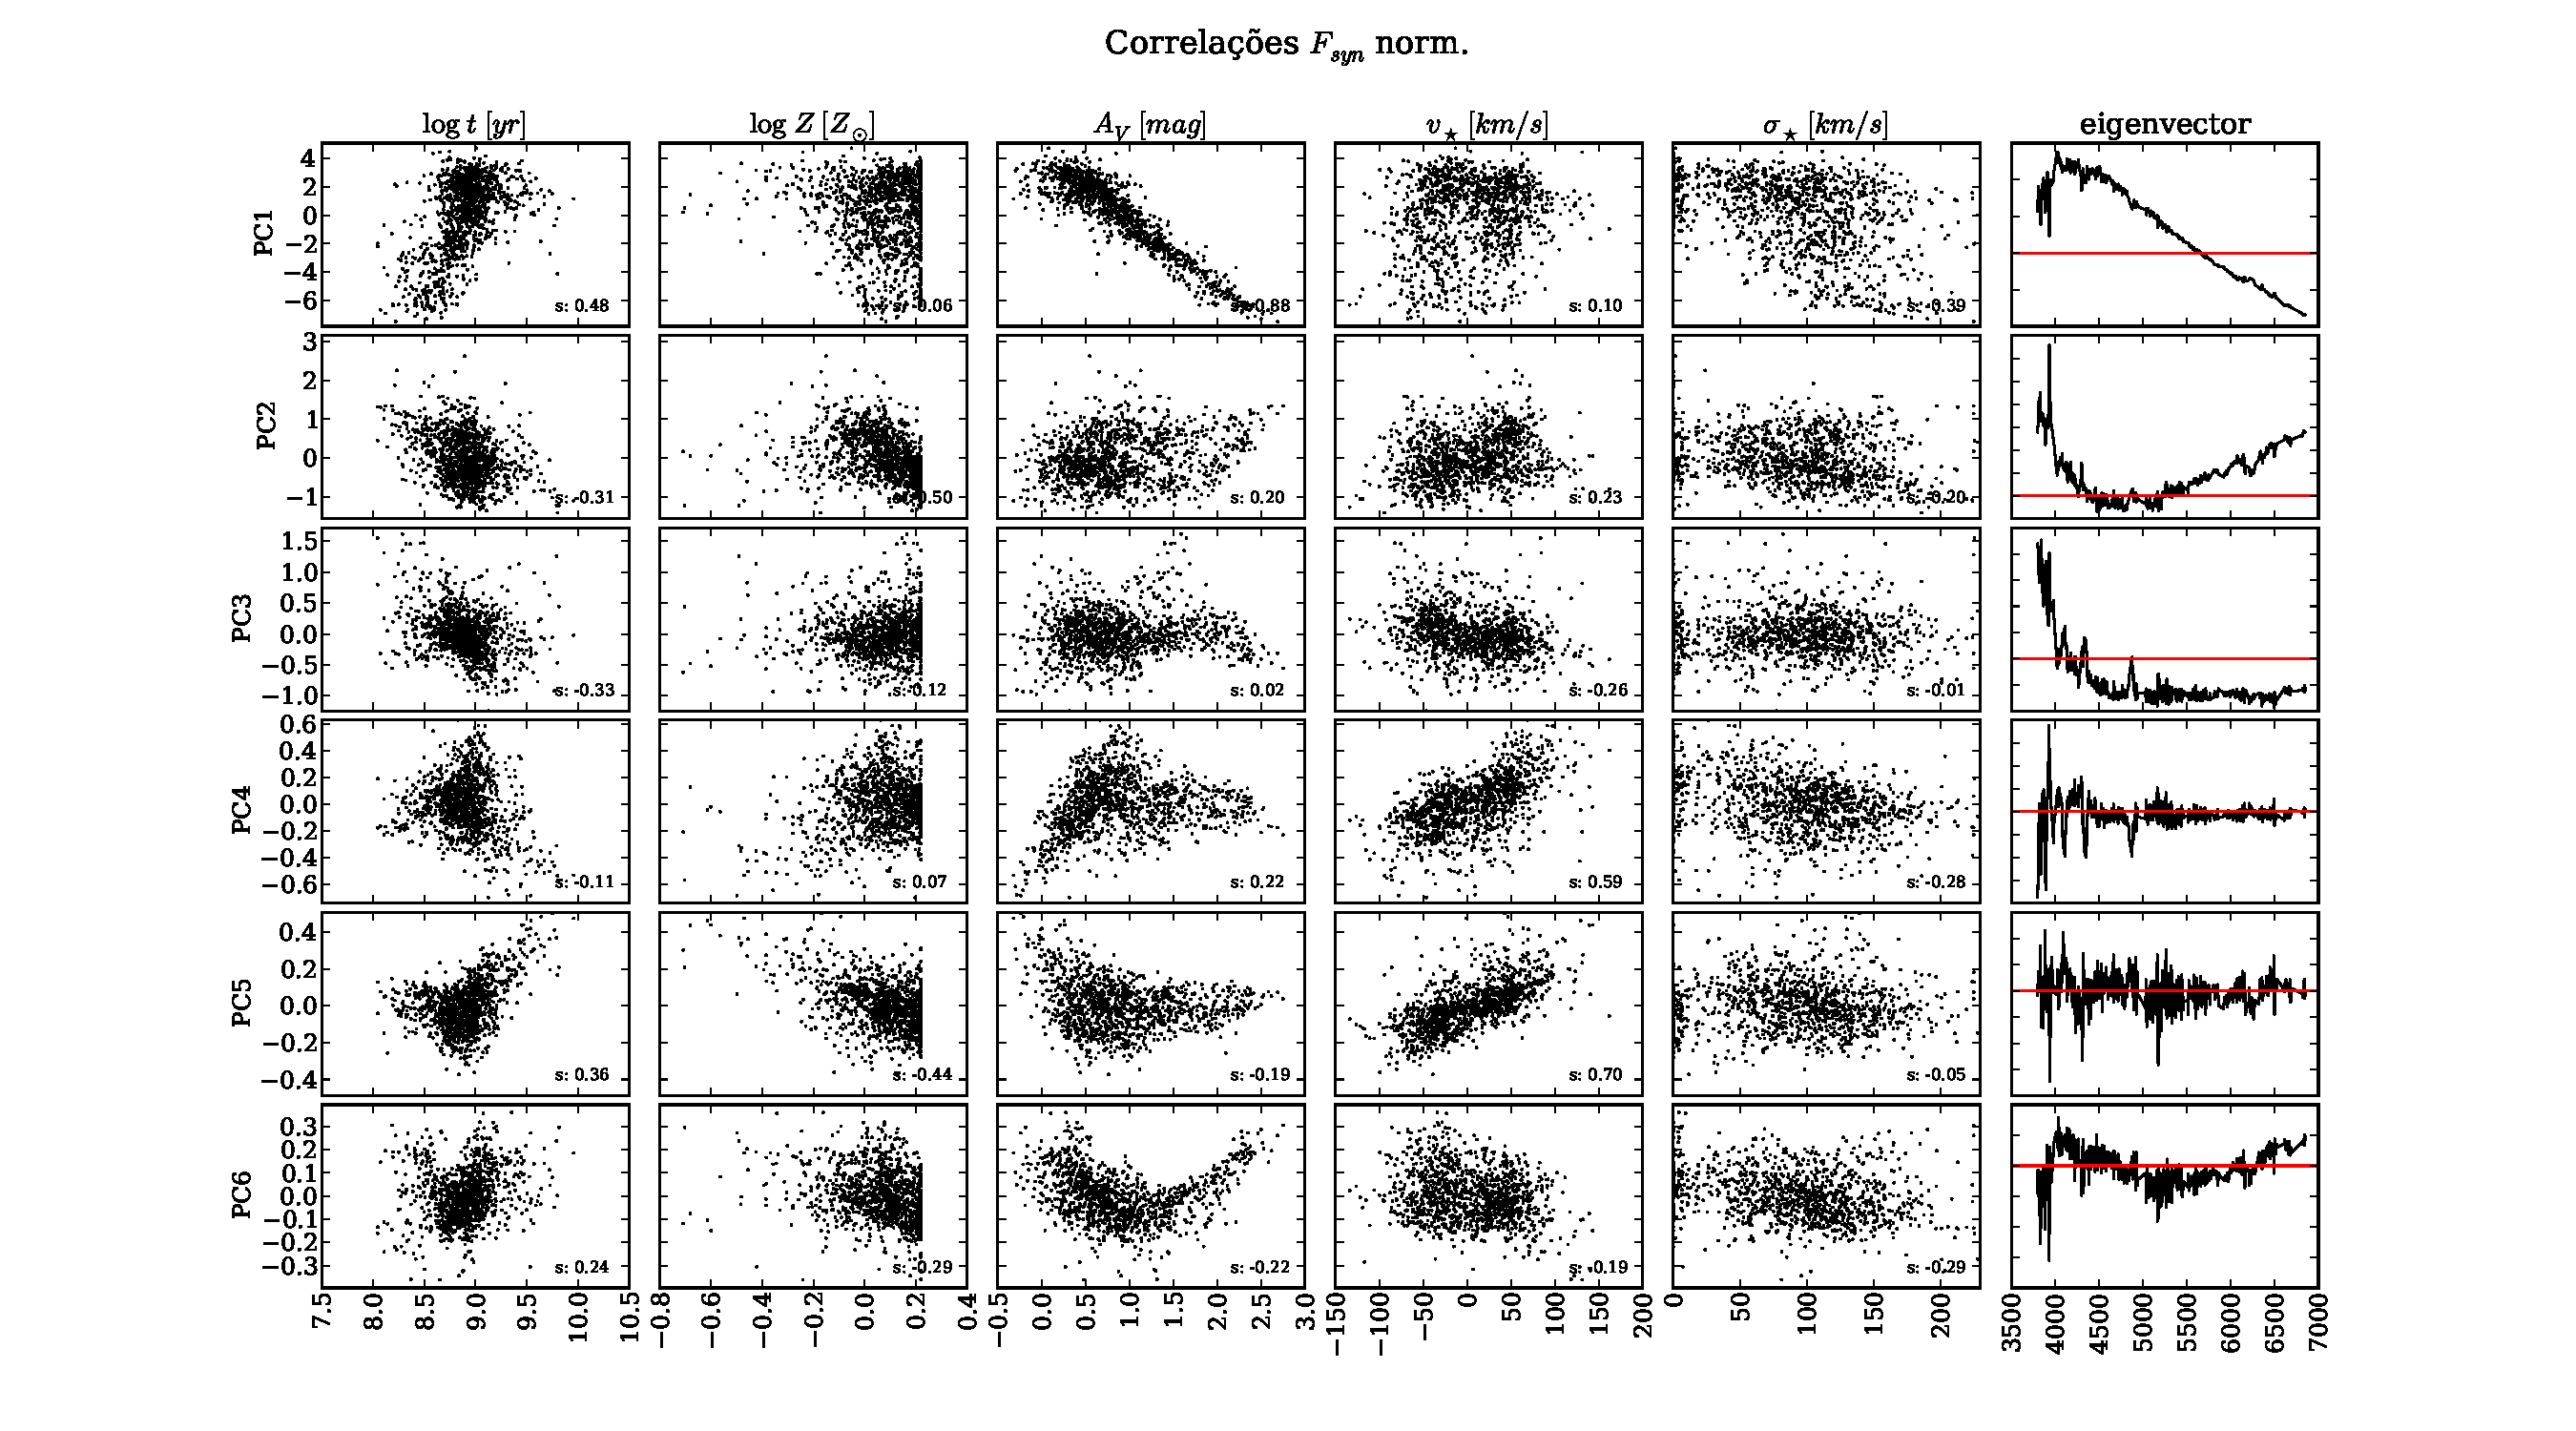
\includegraphics[width=1.3\textwidth, angle=-90]{figuras/K0802-correl-f_syn_norm-PCvsPhys.pdf}
	\caption[Correlações PCs vs. par\^ametros f\'isicos - $F_{syn}$ norm. - ARP 220.]
	{Igual a Figura \ref{fig:K0008correfsynnorm} para a galáxia ARP 220.}
    \label{fig:K0802correfsynnorm}
\end{figure}

% End of this chapter
